\documentclass{wissdoc}
% Autor: Roland Bless 1996-2009, bless <at> kit.edu
% ----------------------------------------------------------------
% Diplomarbeit - Hauptdokument
% ----------------------------------------------------------------
%%
%% $Id: thesis.tex 65 2012-05-10 10:32:11Z bless $
%%
% wissdoc Optionen: draft, relaxed, pdf --> siehe wissdoc.cls
% ------------------------------------------------------------------
% Weitere packages: (Dokumentation dazu durch "latex <package>.dtx")
\usepackage[numbers,sort&compress]{natbib}
\usepackage{url}
\usepackage{amssymb}
%\usepackage{graphicx} 
% \usepackage{varioref}
% \usepackage{verbatim}
% \usepackage{float}    %z.B. \floatstyle{ruled}\restylefloat{figure}
% \usepackage{subfigure}
% \usepackage{fancybox} % für schattierte,ovale Boxen etc.
% \usepackage{tabularx} % automatische Spaltenbreite
% \usepackage{supertab} % mehrseitige Tabellen
% \usepackage[svnon,svnfoot]{svnver} % SVN Versionsinformation 
%% ---------------- end of usepackages -------------

%\svnversion{$Id: thesis.tex 65 2012-05-10 10:32:11Z bless $} % In case that you want to include version information in the footer

%% Informationen für die PDF-Datei
\hypersetup{
 pdfauthor={N.N.},
 pdftitle={Not set}
 pdfsubject={Not set},
 pdfkeywords={Not set}
}

% Macros, nicht unbedingt notwendig
%%%%%%%%%%%%%%%%%%%%%%%%%%%%%%%%%%%%%%%%%%%%%%%%%%%%%%%%%%
% macros.tex -- einige mehr oder weniger nuetzliche Makros
% Autor: Roland Bless 1998
%%%%%%%%%%%%%%%%%%%%%%%%%%%%%%%%%%%%%%%%%%%%%%%%%%%%%%%%%%
% $Id: macros.tex 33 2007-01-23 09:00:59Z bless $
%%%%%%%%%%%%%%%%%%%%%%%%%%%%%%%%%%%%%%%%%%%%%%%%%%%%%%%%%%


%%%%%%%%%%%%%%%%%%%%%%%
% Kommentare 
%%%%%%%%%%%%%%%%%%%%%%%
\ifnotdraftelse{
\newcommand{\Kommentar}[1]{}
}{\newcommand{\Kommentar}[1]{{\em #1}}}
% Alles innerhalb von \Hide{} oder \ignore{} 
% wird von LaTeX komplett ignoriert (wie ein Kommentar)
\newcommand{\Hide}[1]{}
\let\ignore\Hide

%%%%%%%%%%%%%%%%%%%%%%%%%
% Leere Seite ohne Seitennummer, wird aber gezaehlt
%%%%%%%%%%%%%%%%%%%%%%%%%

\newcommand{\leereseite}{% Leerseite ohne Seitennummer, n�chste Seite rechts (wenn 2-seitig)
 \clearpage{\pagestyle{empty}\cleardoublepage}
}
%%%%%%%%%%%%%%%%%%%%%%%%%%
% Flattersatz rechts und Silbentrennung, Leerraum nach rechts maximal 1cm
%%%%%%%%%%%%%%%%%%%%%%%%%%
\makeatletter
\newcommand{\myraggedright}{%
 \let\\\@centercr\@rightskip 0pt plus 1cm
 \rightskip\@rightskip
  \leftskip\z@skip
  \parindent\z@
  \spaceskip=.3333em
  \xspaceskip=.5em}
\makeatother

\makeatletter
\newcommand{\mynewline}{%
 \@centercr\@rightskip 0pt plus 1cm
}
\makeatother


%%%%%%%%%%%%%%%%%%%%%%%%%%
% F�r Index
%%%%%%%%%%%%%%%%%%%%%%%%%%
\makeatletter
\def\mydotfill{\leavevmode\xleaders\hb@xt@ .44em{\hss.\hss}\hfill\kern\z@}
\makeatother
\def\bold#1{{\bfseries #1}}
\newbox\dbox \setbox\dbox=\hbox to .4em{\hss.\hss} % dot box for leaders
\newskip\rrskipb \rrskipb=.5em plus3em % ragged right space before break
\newskip\rrskipa \rrskipa=-.17em plus -3em minus.11em % ditto, after
\newskip\rlskipa \rlskipa=0pt plus3em % ragged left space after break
\newskip\rlskipb \rlskipb=.33em plus-3em minus.11em % ragged left before break
\newskip\lskip \lskip=3.3\wd\dbox plus1fil minus.3\wd\dbox % for leaders
\newskip \lskipa \lskipa=-2.67em plus -3em minus.11em %after leaders
\mathchardef\rlpen=1000 \mathchardef\leadpen=600
\def\rrspace{\nobreak\hskip\rrskipb\penalty0\hskip\rrskipa}
\def\rlspace{\penalty\rlpen\hskip\rlskipb\vadjust{}\nobreak\hskip\rlskipa}
\let\indexbreak\rlspace
\def\raggedurl{\penalty10000 \hskip.5em plus15em \penalty0 \hskip-.17em plus-15em minus.11em}
\def\raggeditems{\nobreak\hskip\rrskipb \penalty\leadpen \hskip\rrskipa %
\vadjust{}\nobreak\leaders\copy\dbox\hskip\lskip %
\kern3em \penalty\leadpen \hskip\lskipa %
\vadjust{}\nobreak\hskip\rlskipa}
\renewcommand*\see[2]{\rlspace\emph{\seename}~#1} % from makeidx.sty

%%%%%%%%%%%%%%%%%%%%%%%%%%
% Neue Seite rechts, leere linke Seite ohne Headings
%%%%%%%%%%%%%%%%%%%%%%%%%%
\newcommand{\xcleardoublepage}
{{\pagestyle{empty}\cleardoublepage}}

%%%%%%%%%%%%%%%%%%%%%%%%%%
% Tabellenspaltentypen (benoetigt colortbl)
%%%%%%%%%%%%%%%%%%%%%%%%%%
\newcommand{\PBS}[1]{\let\temp=\\#1\let\\=\temp}
\newcolumntype{y}{>{\PBS{\raggedright\hspace{0pt}}}p{1.35cm}}
\newcolumntype{z}{>{\PBS{\raggedright\hspace{0pt}}}p{2.5cm}}
\newcolumntype{q}{>{\PBS{\raggedright\hspace{0pt}}}p{6.5cm}}
\newcolumntype{g}{>{\columncolor[gray]{0.8}}c} % Grau
\newcolumntype{G}{>{\columncolor[gray]{0.9}}c} % helleres Grau

%%%%%%%%%%%%%%%%%%%%%%%%%%
% Anf�hrungszeichen oben und unten
%%%%%%%%%%%%%%%%%%%%%%%%%%
\newcommand{\anf}[1]{"`{#1}"'}

%%%%%%%%%%%%%%%%%%%%%%%%%%
% Tiefstellen von Text
%%%%%%%%%%%%%%%%%%%%%%%%%%
% S\tl{0} setzt die 0 unter das S (ohne Mathemodus!)
% zum Hochstellen gibt es uebrigens \textsuperscript
\makeatletter
\DeclareRobustCommand*\textlowerscript[1]{%
  \@textlowerscript{\selectfont#1}}
\def\@textlowerscript#1{%
  {\m@th\ensuremath{_{\mbox{\fontsize\sf@size\z@#1}}}}}
\let\tl\textlowerscript
\let\ts\textsuperscript
\makeatother

%%%%%%%%%%%%%%%%%%%%%%%%%%
% Gau�-Klammern
%%%%%%%%%%%%%%%%%%%%%%%%%%
\newcommand{\ceil}[1]{\lceil{#1}\rceil}
\newcommand{\floor}[1]{\lfloor{#1}\rfloor}

%%%%%%%%%%%%%%%%%%%%%%%%%%
% Average Operator (analog zu min, max)
%%%%%%%%%%%%%%%%%%%%%%%%%%
\def\avg{\mathop{\mathgroup\symoperators avg}}

%%%%%%%%%%%%%%%%%%%%%%%%%%
% Wortabk�rzungen
%%%%%%%%%%%%%%%%%%%%%%%%%%
\def\zB{z.\,B.\ }
\def\dh{d.\,h.\ }
\def\ua{u.\,a.\ }
\def\su{s.\,u.\ }
\newcommand{\bzw}{bzw.\ }

%%%%%%%%%%%%%%%%%%%%%%%%%%%%%%%%%%%
% Einbinden von Graphiken
%%%%%%%%%%%%%%%%%%%%%%%%%%%%%%%%%%%
% global scaling factor
\def\gsf{0.9}
%% Graphik, 
%% 3 Argumente: Datei, Label, Unterschrift
\newcommand{\Abbildung}[3]{%
\begin{figure}[tbh] %
\centerline{\scalebox{\gsf}{\includegraphics*{#1}}} %
\caption{#3} %
\label{#2} %
\end{figure} %
}
\let\Abb\Abbildung
%% Abbps
%% Graphik, skaliert, Angabe der Position
%% 5 Argumente: Position, Breite (0 bis 1.0), Datei, Label, Unterschrift
\newcommand{\Abbildungps}[5]{%
\begin{figure}[#1]%
\begin{center}
\scalebox{\gsf}{\includegraphics*[width=#2\textwidth]{#3}}%
\caption{#5}%
\label{#4}%
\end{center}
\end{figure}%
}
\let\Abbps\Abbildungps
%% Graphik, Angabe der Position, frei w�hlbares Argument f�r includegraphics
%% 5 Argumente: Position, Optionen, Datei, Label, Unterschrift
\newcommand{\Abbildungpf}[5]{%
\begin{figure}[#1]%
\begin{center}
\scalebox{\gsf}{\includegraphics*[#2]{#3}}%
\caption{#5}%
\label{#4}%
\end{center}
\end{figure}%
}
\let\Abbpf\Abbildungpf

%%
% Anmerkung: \resizebox{x}{y}{box} skaliert die box auf Breite x und H�he y,
%            ist x oder y ein !, dann wird das uspr�ngliche 
%            Seitenverh�ltnis beibehalten.
%            \rescalebox funktioniert �hnlich, nur das dort ein Faktor
%            statt einer Dimension angegeben wird.
%%
% \Abbps{Position}{Breite in Bruchteilen der Textbreite}{Dateiname}{Label}{Bildunterschrift}
%

\newcommand{\refAbb}[1]{%
s.~Abbildung \ref{#1}}

%%%%%%%%%%%%%%%%%%%%
%% end of macros.tex
%%%%%%%%%%%%%%%%%%%%

% Print URLs not in Typewriter Font
\def\UrlFont{\rm}

\newcommand{\blankpage}{% Leerseite ohne Seitennummer, nächste Seite rechts
 \clearpage{\pagestyle{empty}\cleardoublepage}
}

%% Einstellungen für das gesamte Dokument

% Trennhilfen
% Wichtig! 
% Im ngerman-paket sind zusätzlich folgende Trennhinweise enthalten:
% "- = zusätzliche Trennstelle
% "| = Vermeidung von Ligaturen und mögliche Trennung (bsp: Schaf"|fell)
% "~ = Bindestrich an dem keine Trennung erlaubt ist (bsp: bergauf und "~ab)
% "= = Bindestrich bei dem Worte vor und dahinter getrennt werden dürfen
% "" = Trennstelle ohne Erzeugung eines Trennstrichs (bsp: und/""oder)

% Trennhinweise fuer Woerter hier beschreiben
\hyphenation{
% Pro-to-koll-in-stan-zen
% Ma-na-ge-ment  Netz-werk-ele-men-ten
% Netz-werk Netz-werk-re-ser-vie-rung
% Netz-werk-adap-ter Fein-ju-stier-ung
% Da-ten-strom-spe-zi-fi-ka-tion Pa-ket-rumpf
% Kon-troll-in-stanz
}

% Index-Datei öffnen
\ifnotdraft{\makeindex}
%%%%%%%%%%%%%% includeonly %%%%%%%%%%%%%%%%%%%
% Es werden nur die Teile eingebunden, die hier 
% aufgefuehrt sind!
\includeonly{%
titelseite,
erklaerung,
einleitung,
grundlagen,
analyse,
noChanges,
softwareChanges,
hardwareChanges,
lora,
tweaks,
%range,
%realworld,
fazit
}
%%%%%%%%%%%%%%%%%%%%%%%%%%%%%%%%%%%%%%%%%%%%%%
\begin{document}

\frontmatter
\pagenumbering{roman}
\ifnotdraft{
 %% Titelseite
%% Vorlage $Id: titelseite.tex 61 2012-05-03 13:58:03Z bless $

\def\usesf{}
\let\usesf\sffamily % diese Zeile auskommentieren für normalen TeX Font

\newsavebox{\Erstgutachter}
\savebox{\Erstgutachter}{\usesf Prof.~Dr.~H.~Schmeck}
\newsavebox{\Zweitgutachter}
\savebox{\Zweitgutachter}{\usesf Prof.~Dr.~?.~?????????}

\begin{titlepage}
\setlength{\unitlength}{1pt}
\begin{picture}(0,0)(85,770)

\includegraphics[width=\paperwidth]{logos/KIT_Deckblatt}
\end{picture}

\thispagestyle{empty}

%\begin{titlepage}
%%\let\footnotesize\small \let\footnoterule\relax
\begin{center}
\hbox{}
\vfill
{\usesf
{\huge\bfseries Energieoptimierung WLAN-basierter Ortungseinheiten \par}
\vskip 1.8cm
Masterarbeit\\
von\\[2mm]
\vskip 1cm

{\large\bfseries Marius Wodtke\\}
\vskip 1.2cm
Institut für Angewandte Informatik und Formale Beschreibungsverfahren (AIFB)\\
der Fakultät für Informatik\\
%Universität Karlsruhe (TH)\\[2ex]
\vskip 3cm
\begin{tabular}{p{5.5cm}l}
Erstgutachter: & \usebox{\Erstgutachter} \\
Zweitgutachter: & \usebox{\Zweitgutachter} \\
Betreuender~Mitarbeiter: & Dipl.-Inform.~K.~Bao \\
\end{tabular}
\vskip 3cm
Bearbeitungszeit:\qquad 01.~April~2017 -- 31.~Oktober~2017
}
\end{center}
\vfill
\end{titlepage}
%% Titelseite Ende


%%% Local Variables: 
%%% mode: latex
%%% TeX-master: "thesis"
%%% End: 

 \blankpage % Leerseite auf Titelrückseite
 %
 % Die folgende Erklärung ist für Diplomarbeiten Pflicht
 % (siehe Prüfungsordnung), für Studienarbeiten nicht notwendig
 \thispagestyle{empty}
\vspace*{32\baselineskip}
\hbox to \textwidth{\hrulefill}
\par
Ich erkl�re hiermit, dass ich die vorliegende Arbeit selbst�ndig verfasst und
keine anderen als die angegebenen Quellen und Hilfsmittel benutzt, 
die w�rtlich oder inhaltlich �bernommenen Stellen als solche kenntlich 
gemacht und die Satzung des KIT zur Sicherung guter wissenschaftlicher 
Praxis in der jeweils g�ltigen Fassung beachtet habe.

\vspace*{2cm}
Karlsruhe, den ??. ?????? 201?\hfill \hbox to 8cm{\hrulefill}

%%%%%%%%%%%%%%%%%%%%%%%%%%%%%%%%%%%%%%%%%%%%%%%%%%%%%%%%%%%%%%%%%%%%%%%%
%% Hinweis:
%%
%% Diese Erkl�rung wird von der Pr�fungsordnung f�r Diplom-, Master,
%% und Bachelorarbeiten verlangt und ist zu unterschreiben. 
%% F�r Studienarbeiten ist diese Erkl�rung nicht zwingend notwendig, 
%% schadet aber auch nicht.
%%%%%%%%%%%%%%%%%%%%%%%%%%%%%%%%%%%%%%%%%%%%%%%%%%%%%%%%%%%%%%%%%%%%%%%%
\clearpage







 \blankpage % Leerseite auf Erklärungsrückseite
}
%
%% *************** Hier geht's ab ****************
%% ++++++++++++++++++++++++++++++++++++++++++
%% Verzeichnisse
%% ++++++++++++++++++++++++++++++++++++++++++
\ifnotdraft{
{\parskip 0pt\tableofcontents} % toc bitte einzeilig
\blankpage
%\listoffigures
%\blankpage
%\listoftables
%\blankpage
}


%% ++++++++++++++++++++++++++++++++++++++++++
%% Hauptteil
%% ++++++++++++++++++++++++++++++++++++++++++
\graphicspath{{Bilder/}}

\mainmatter
\pagenumbering{arabic}
\chapter{Einleitung}
\label{ch:Einleitung}
Während die Ortung im Außenbereich fest in der Hand von Satellitennavigationssystemen wie dem Global Positioning System (GPS) liegen, existiert für die Ortung im Innenraum eine Vielzahl verschiedener Technologien. Neben Technologien wie Bluetooth, Radio Frequency Identification (RFID) und Ultra Wide Band (UWB) weckt WLAN wegen seiner großen Verbreitung immer wieder Interesse in Forschung und Industrie. 

So hat die Ortung mittels WLAN gerade im medizinischen Bereich durch kommerzielle Lösungen Verbreitung gefunden, Probleme finden sich aber bei Ortungsgenauigkeit gegenüber anderen Techniken und dem vergleichsweise hohen Energieverbrauch des WLAN-Protokolls.
Während sich viele wissenschaftliche Arbeiten der Ortungsgenauigkeit widmen, ist für den alltäglichen Einsatz die kurze Batterielaufzeit der mobilen Einheiten hinderlich, wenn nicht zum Beispiel Smartphones als mobile Einheiten in Frage kommen. 

Auch im Tunnelbau ist eine Ortung von Mitarbeitern und Besuchern von Nöten um in Notfällen bestimmen zu können, ob und wie viele Personen sich im Gefahrenbereich befinden. 
Dies beeinflusst die Arbeit der Rettungskräfte. 
Das veränderliche Umfeld der Baustelle, auf der große Stahl- und Betonelemente bewegt werden, stellt dabei die genaue Ortung mittels Radiowellen vor große Probleme und es wird nur eine Bereichsortung durchgeführt, bei der jede Tunnelröhre in mehrere hundert Meter große Abschnitte aufgeteilt wird und der Wechsel der Mitarbeiter zwischen den Abschnitten beobachtet wird. 
Dies stellt zwar nur eine geringe Genauigkeit dar, erlaubt es aber bei Bränden zu erkennen, welche Personen sich durch die Abschnitte Richtung Ausgang bewegen und welche in ihrem Abschnitt verharren. 
Solche Personen sind vermutlich bewegungsunfähig oder eingeschlossen.


\section{Bisherige Situation}
Die Ortung wird derzeit bei der Ed. Züblin AG mittels Bluetooth durchgeführt. 
Dabei sind die Basisstationen eigenständige Bluetooth-Einheiten, die mit dem Ethernet Backbone verbunden sind.
Als mobile Einheiten kommen sowohl batteriebetriebene "`Tags"' als auch Smartphones zum Einsatz. 
Das zentrale Sicherheitssystem fragt die gesehenen mobilen Einheiten bei den Basisstationen an und bereitet die Ergebnisse graphisch auf.

Der Tunnel wird in Bereiche zu circa 500 Meter aufgeteilt, die Tunnelbohrmaschine (TBM) stellt dabei einen Sonderbereich dar, weil sie sich im Gegensatz zu den anderen Bereichen langsam bewegt. 
Neue Bereiche werden hinter der TBM eingefügt und sind dann stationär.

Die Bluetooth-Basisstationen werden in Kästen verstaut, die weitere notwendige Technik, wie etwa ein Notfalltelefon, enthalten.
Weil diese Kästen nur etwa alle 500 Meter montiert sind, existieren große Lücken in denen die mobilen Einheiten nicht geortet werden.
Eine mobile Einheit wird im System so lange im selben Bereich angezeigt, bis sie wieder von einer Basisstation erkannt wird.

Wird die mobile Einheit von der Erfassungseinheit vor dem Portal (Tunneleingang) erkannt gilt sie als außerhalb des Tunnels.
Abbildung \ref{fig:bisherige} zeigt die bisherige Situation mit Bluetooth-Basisstaionen. 
Die Reichweite der der Basistationen ist dabei nicht maßstabsgetreu.

\begin{figure}[h]
  \centering
	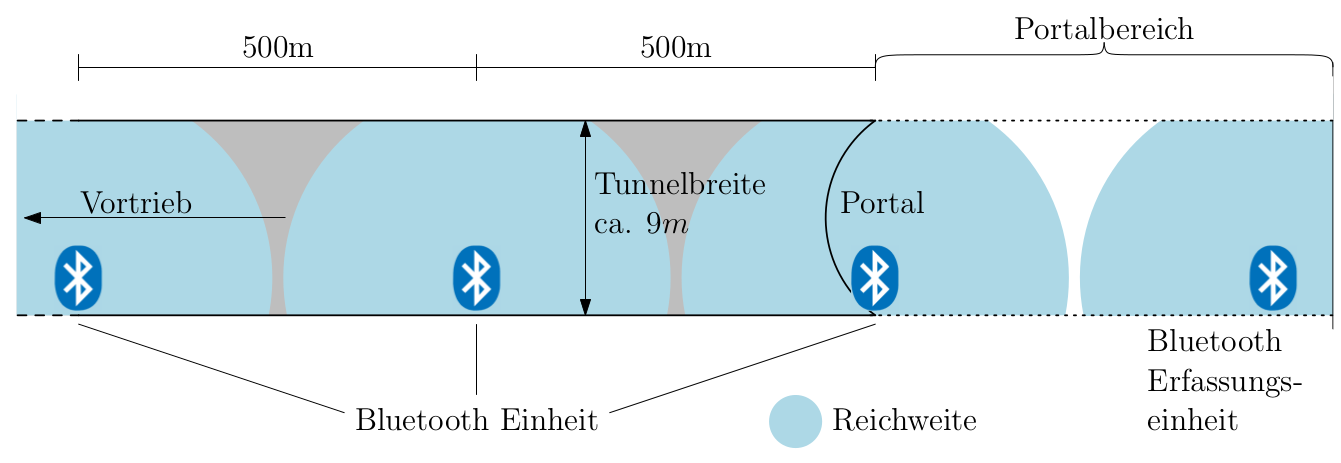
\includegraphics[width=\textwidth]{images/bisherige.png}
  \caption{Bereichsortung mit Bluetooth, aus \cite{maurer2016unterstuetzung}.}
  \label{fig:bisherige}
\end{figure}

 
\section{Umgebung für funkbasierte Ortung}
Als Versuchsumgebung dient die Tunnelbaustelle Rastatt.
Dort gelten die Positionen der Kästen für die Technik als unveränderlich.
Nur sie bieten Strom, Netzwerkanbindung (LAN) und Schutz vor dem Baustellenumfeld.
Für Funkprotokolle, die weniger als 250 Meter Reichweite entfalten muss daher mit Erfasssungslücken gerechnet werden.
Auf der TBM und anderen technischen Fahrzeugen sind jedoch mehr Basisstationen möglich.

Es existiert bereits ein WLAN-Netzwerk, dessen Access Points als Basisstationen genutzt werden können.
Es handelt sich um APs der Firma Lancom, diese stellt auch ein Modell LN-862 für Versuche.
Für zukünftige Baustellen soll der Abstand der Versorgungskästen auf 250 Meter sinken. 
Diese Situation ist in Abbildung \ref{fig:zukuenftige} skizziert.

\begin{figure}[h]
  \centering
	\includegraphics[width=\textwidth]{images/zukuenftige.eps}
  \caption{Zukünftige Situation der Tunnelbaustellen.}
  \label{fig:zukuenftige}
\end{figure}

\section{Problemstellung}
Es muss ein System geschaffen werden, welches Mitarbeiter einem 250 Meter langen Abschnitt innerhalb eines im Bau befindlichen Tunnels zuordnet.
Dazu soll keine Nutzerinteraktion nötig sein, der Nutzer wird wird über eine mobile Einheit geortet.
Die Ortung muss unterirdisch funktionieren und robust gegenüber Stahlhindernissen sein.
Außerdem können Basisstation für die Ortung nur alle 250 Meter platziert werden.


\section{Zielsetzung der Arbeit}
\label{ch:Einleitung:sec:Zielsetzung}
Ziel der Arbeit soll der Entwurf und die Implementierung eines Bereichsortungssystems für Personen in Tunnelanlagen sein. 
Bei einem Bereichsortungssystem handelt es sich um ein Ortungssystem, bei dem die Positionen nicht genau bestimmt werden. 
Stattdessen wird das Areal, auf dem geortet werden soll, in einzelne Bereiche unterteilt und jede mobile Einheit beim Vorgang des Ortens einem dieser Bereiche zugeordnet.

Diese Arbeit grenzt sich von vorherigen Arbeiten dadurch ab, dass die Laufzeit beziehungsweise der Energieverbrauch der mobilen Einheiten im Vordergrund steht. 
Ziel dieser Arbeit ist eine mehrmonatige Laufzeit der mobilen Einheiten. 

Für diese Arbeit werden mehrere Prototypen für mobile Einheiten entwickelt und auf ihre Charakteristik bezüglich des Energieverbrauchs und der Erkennungszuverlässigkeit untersucht.
Der Entwurfsraum umfasst dabei die Hardware und Software der mobilen Enheit sowie die Implementierung des Ortungsdienstes. 
Die für die Funktechnologie benötigte Infrastruktur wird jeweils als gegeben angenommen.


\section{Anforderungen an das Bereichsortungssystem}
\label{ch:Einleitung:sec:Anforderungen}
Da es sich um ein Bereichsortungssystem handeln soll, werden keine direkten Anforderungen an die Genauigkeit der Ortung gestellt. 
Jedoch soll ein klarer Wechsel zwischen zwei Bereichen, und damit zwei Basisstationen, zuverlässig erkannt werden. 
Die mobilen Einheiten sollen von Personen um den Hals getragen werden können. 
Dies bedingt ein geringes Gewicht des Akkus, gleichzeitig soll aber die Laufzeit der mobilen Einheit maximiert werden, sodass ein Akku mit möglichst großer Kapazität gewählt werden sollte.
Zuletzt soll unter Rücksichtnahme auf das beschriebene Szenario die Komplexität der benötigten IT-Infrastruktur so gering wie möglich gehalten werden um ein stabiles und kostengünstiges System zu garantieren. 


\section{Gliederung der Arbeit}
\label{ch:Einleitung:sec:Gliederung}
Nachdem zunächst in Kapitel \ref{ch:Grundlagen} die Grundlagen der funkbasierten Ortung und der verwendeten Funkprotokolle behandelt werden, wird in Kapitel \ref{ch:Analyse} das Problem analysiert und verwandte Arbeiten aufgezeigt.
Kapitel \ref{ch:Implementierung} beschäftigt sich mit der Implementierung und Untersuchung der Prototypen. 
Das Fazit in Kapitel \ref{ch:Fazit} fasst die Arbeit noch einmal zusammen, vergleicht und bewertet die Ergebnisse.
  % Einleitung
\chapter{Grundlagen}
\label{ch:Grundlagen}

\section{Klassifikation von Ortungssystemen}
%% ==============================
\label{ch:Einleitung:sec:Ortungssysteme}
Die Klassifikation von Ortungssystemen auf Funkbasis kann neben dem verwendeten Protokoll anhand der Topologie, dem Lokalisierungsprinzip und der gemessenen Größen durchgeführt werden \cite{liu2007survey}.
Außerdem wird zwischen zweidimensionaler und dreidimensionaler Lokalisierung unterschieden.

\subsection{Funkprotokoll-Standards}
Prinzipiell lassen sich verwendete Frequenzen, Modulationsverfahren und Sendeleistung frei wählen, solange die gesetzlichen Vorgaben für die Sender eingehalten werden. Wenn ein eigenes Protokoll verwendet wird, kann die Kodierung der Informationen frei gewählt werden. 
Ein Beispiel für ein solches Protokoll ist die Ortung mit Ultra-Breitband-Signalen (UWB), mit dem Genauigkeiten im Zentimeterbereich erreicht werden können. Bestehende Protokolle zu verwenden hat dagegen den Vorteil, dass üblicherweise \emph{commodity-of-the-shelf}-Komponenten verwendet werden können, was die Kosten des Systems senkt. Im Gegenzug können für die Genauigkeit wichtige Parameter nicht mehr frei gewählt werden und der \emph{Overhead} des Protokolls muss in Kauf genommen werden. Beispiele für solche Protokolle sind IEEE 802.11 (WLAN), Bluetooth und Radio Frequency Identification (RFID).

\subsection{Topologie}
Die Topologie hat zwei Dimensionen, Fernlokalisierung versus Selbstlokalisierung und direkt versus indirekt und beschreibt wie Basisstationen und mobile Einheiten zusammenwirken. 
Alle besprochenen Topologien sind in Abbildung \ref{fig:topo} veranschaulicht, gewellte Pfeile stellen hier zu messende Signale dar, gerade Pfeile sind gerichtete Datenverbindungen.\\

\subsubsection{Direkte Fernlokalisierung} 
Bei der direkten Fernlokalisierung werden von mobilen Einheiten gesendete Signale an Basisstationen gemessen und die Ergebnisse an einen zentralen Ortungsdienst weitergegeben, dieser führt dann die Lokalisierung durch. Das Ergebnis der Lokalisierung ist nur zentral verfügbar. \\

\subsubsection{Direkte Selbstlokalisierung} 
Bei der direkten Selbstlokalisierung senden hingegen die Basisstationen und die mobilen Einheiten messen die eingehenden Signale. Anhand der Messergebnisse bestimmt jede mobile Einheit seine Position. 
Die Ergebnisse der Lokalisierung sind anschließend nur auf der mobilen Einheit verfügbar. \\

\subsubsection{Indirekte Fernlokalisierung} 
Die indirekte Fernlokalisierung gleicht der direkten Selbstlokalisierung, allerdings besteht zusätzlich eine Datenverbindung zu einem zentralen Ortungsdienstes, dem die berechnete Position mitgeteilt wird. 
Das Ergebnis steht nach kurzer Verzögerung sowohl auf der mobilen Einheit als auch zentral zur Verfügung.
Optional können dort die Daten von anderen mobilen Einheiten abgerufen werden um sich über deren Positionen zu informieren. \\

\subsubsection{Indirekte Selbstlokalisierung} 
Auch die indirekte Selbstlokalisierung erweitert die direkte Fernlokalisierung um eine Datenverbindung zwischen mobiler Einheit und zentralem Ortungsdienst. 
So kann sie sich über die eigene und eventuelle auch andere mobile Einheiten informieren. 
Dies kann insbesondere bei der Verwendung von Mischtechnologien notwendig sein, wenn die zur Ortung genutzte Technik es nicht erlaubt an den mobilen Einheiten zu empfangen, aber dennoch eine Selbstlokalisierung durchgeführt werden soll.

\subsubsection{Lokalisierung ohne Basisstationen} 
Die mobilen Einheiten können sich auch gegenseitig lokalisieren, dazu messen sie die Distanz zu anderen mobilen Einheiten.
Sie können diese Ergebnisse dann wiederum anderen mobilen Stationen mitteilen um so indirekt mit weiteren Referenzen die Lokalisierung zu präzisieren. 
Dadurch ensteht eine maßstabslose Karte, die die relative Position der mobilen Einheit zu den anderen mobilen Einheiten erfasst.
Diese kann zusätzlich an einen zentralen Ortungsdienst versendet werden um sie dort verfügbar zu machen.

\subsubsection{Hybride Topologie}
In einer hybriden Topologie orten sich die mobilen Einheiten gegenseitig, werden dabei aber von wenigen Basisstationen unterstützt.
Diese Basisstationen geben ihre feste Position bekannt, dadurch ist es möglich der enstehenden Karte Punkte für die Ausrichtung und Skalierung hinzuzufügen.
Außerdem können sie mit dem zentralen Ortungsdienst kommunizieren um eine indirekte Fernlokalisierung mittels der durch die mobilen Einheiten propagierten Karten eine indirekte Fernlokaliserung durchzuführen.

\begin{figure}[h!]
	\centering

	\begin{tabular}{cc}
		\includegraphics[width=0.4\textwidth]{images/direkteselbst.eps} & \includegraphics[width=0.4\textwidth]{images/indirekteselbst.eps} \\
		(a) Direkte Selbstlokalisierung & (b) Indirekte Selbstlokalisierung \\
		\includegraphics[width=0.4\textwidth]{images/direktefern.eps} & \includegraphics[width=0.4\textwidth]{images/indirektefern.eps} \\
		(c) Direkte Fernlokalisierung & (d) Indirekte Fernlokalisierung \\
		\includegraphics[width=0.25\textwidth]{images/ohnebasis.eps} & \includegraphics[width=0.4\textwidth]{images/hybrid.eps} \\
		(e) Lokalisierung ohne Basisstation & (f) Hybride Topologie \\
	\end{tabular}
	\caption{Topologien für die Lokalisierung}
	\label{fig:topo}
\end{figure}

\subsection{Lokalisierungsprinzip}
Das einfachste Lokalisierungsprinzip ist das Umgebungsprinzip, hier wird eine mobile Einheit der Basisstation mit dem stärksten Signal zugeordnet. 
Die Basisstation kann sowohl als Sender als auch als Empfänger auftreten. 
Die gewonnene Position ist dabei nur symbolisch und ihre Genauigkeit ist abhängig von der Dichte des Netzes. 
Für eine erfolgreiche Lokalisierung muss nur eine Basisstation in Reichweite der mobilen Einheit sein, was diese Möglichkeit auch in komplexeren Lokalisierungsprinzipien zu einer sinnvollen Ausweichmöglichkeit macht, falls nicht genügend Basisstationen in Reichweite sind. \\
Die geometrische Bestimmung der Position einer mobilen Einheit mit drei oder mehr Basisstationen nennt man Trilateration. Dabei wird üblicherweise für jede Basisstation die Distanz zur mobilen Einheit bestimmt, anschließend wird ein Kreis mit der gemessenen Distanz um jede Basisstation gebildet und der Schnittpunkt der drei Kreise bestimmt die Position der mobilen Einheit. Da die Distanzen aus den gemessenen Signalparametern geschätzt werden müssen sind sie fehlerbehaftet und es ergibt sich oft kein eindeutiger Schnittpunkt, dann wird zum Beispiel die Mitte der Schnittpunkte gewählt. \\
Die geometrische Bestimmung ist ebenfalls über die Berechnung der Winkel zu den Basisstationen möglich, dies nennt man Triangulation. Der Winkel kann zum Beispiel über die zeitliche Differenz der ankommenden Signale an den synchronisierten Basisstationen bestimmt werden, dann wird von jeder Basisstation aus eine Halbgerade in diesem Winkel gefällt und der Schnittpunkt bestimmt die Position der mobilen Einheit. %TODO fällen?
Wenn mit gerichteten Antennen gearbeitet wird, kann der Winkel des eingehenden Signals direkt bestimmt werden, dann müssen nur zwei Basisstationen in Reichweite sein um die mobile Einheit zu lokalisieren. \\
Das aufwendigste Lokalisierungsprinzip ist die Szenenanalyse. Hier werden zunächst in einer \emph{Offline-Phase} Vektoren $(m_1,m_2,...,m_n,p_x,p_y,p_z)^T$ aus Messgrößen und Positionsmarken gesammelt, anhand dieser Fingerabdrücke werden dann in der Online-Phase die Positionen neuer Messergebnisse bestimmt. Üblicherweise kommen dabei Verfahren des maschinellen Lernens wie \emph{k-Nearest-Neighbour}, \emph{Neuronale Netze} oder \emph{Support Vektor Machines} (SVM) zum Einsatz um die Muster der Fingerabdrücke aus der \emph{Offline-Phase} zu erkennen und die Positionen $(p_x,p_y,p_z)^T$ in der \emph{Online-Phase} aus den gemessenen Größen $(m_1,m_2,...,m_n)^T$ zu schätzen. Im zweidimensionalen Fall wird dabei $p_z = 0$ angenommen.

\subsection{Messgrößen}
Beliebte Messgrößen für die Positionsbestimmung sind Ankunftszeit des Signals (\emph{Time of Arrival}, TOA), die Differenz der Ankuftszeiten (\emph{Time Difference of Arrival}, TDOA), die Paketumlaufzeit (\emph{Roundtrip Time of Flight}, RTOF) und die Stärke des empfangenen Signals (\emph{Received Signal Strength}, RSS). Es existieren aber noch mehr messbare Größen, wie etwa die Messung der empfangenen Phase des Signals (\emph{Received Signal Phase}, RSP) und die Messung des Einfallsswinkel des Signals mit mehreren gerichteten Antennen (\emph{Angle of Arrival}, AOA). \\

\subsubsection{Time of Arrival}
TOA beruht auf der begrenzten Ausbreitungsgeschwindigkeit des Signals, hochfrequente Signale breiten sich mit Lichtgeschwindigkeit $c = 299.792.458\ m/s$, Ultraschall mit Schallgeschwindigkeit $c \approx 343\ m/s$ bei $20^{\ \circ}C$ aus, damit ergibt sich die Distanz $d_i = c\ *\ (t_{empfangen,i} - t_{gesendet})$ mit $i$ sei die empfangende Basisstation. Die Position der mobilen Einheit kann dann mit der Methode der kleinsten Quadrate bestimmt werden, dazu wird die Kostenfunktion $F(x,y,t_{gesendet}) = \sum_{i=1}^{N} {\alpha}^2_i f^2_i(x,y,t_{gesendet})$ mit $f_i(x,y,t_{gesendet}) = d_i - \sqrt{(x_i - x)^2 + (y_i - y)^2}$ und ${\alpha}_i$ sei die Konfidenz von Basisstation $i$, minimiert. Dies erfordert, dass die Basisstationen zeitsynchronisiert sind und $t_{empfangen,i}$ möglichst ohne vorherige Verarbeitung bestimmt wird, um Varianzen zu vermeiden. Zusätzlich ist es von Vorteil, wenn auch die mobile Einheit synchronisiert ist, da dann nur noch mit zwei Variablen optimiert werden muss, $t_{gesendet}$ kann dann entsprechend der Synchronisation und dem Sendeintervall als gegeben angenommen werden. Die Forderung nach Synchronität ist jedoch für $c = 299.792.458\ m/s$ sehr stark, da das Signal nur $3.36\ ns/m$ benötigt und somit bereits kleine zeitliche Ungenauigkeiten große Fehler verursachen und erst durch zusätzliche Messungen oder Glättungstechniken hohe Genauigkeiten erreicht werden können. Skibniewski et al. konnten hohe Genauigkeit durch die Verwendung von Ultraschall erzielen, da sich durch die geringere Ausbreitungsgeschwindigkeit Imperfektionen in der Synchronisierung weniger stark auswirken \cite{skibniewski2009simulation}. 
Bei einer Selbstlokalisierung ist zu beachten, dass $t_{gesendet}$ den Sendezeitpunkt der Basisstationen darstellt, sie müssen also entweder alle gleichzeitig auf verschiedenen Frequenzen oder in einem vordefinierten Muster nacheinander senden, die Zeitdifferenz des tatsächlichen Sendezeitpunkts zu $t_{gesendet}$ muss dann vom Empfangszeitpunkt $t_{empfangen,i}$ abgezogen werden. \\

\begin{figure}[h]
  \centering
	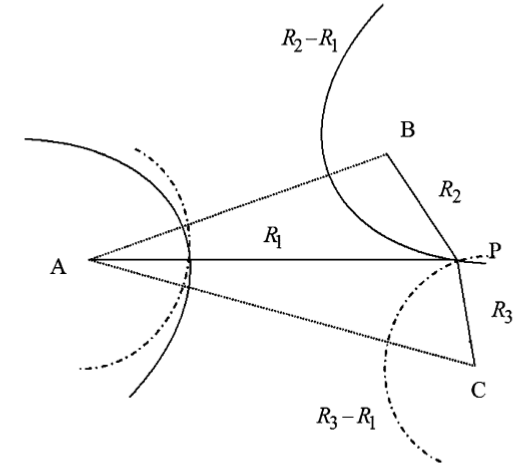
\includegraphics[width=0.5\textwidth]{images/tdoa.png}
  \caption{Positionsbestimmung mit der Differenz der Ankunftszeiten (TDOA), aus \cite{liu2007survey}. A, B und C sind die Basisstationen, die Distanzen $R_x$ werden für die Bestimmung der Position P der mobilen Einheit berechnet.}
  \label{fig:tdoa}
\end{figure}


\subsubsection{Time Difference of Arrival}
Bei TDOA wird statt der direkten Ankunftszeiten die Differenz der Ankunftszeiten gemessen, dies erfordert üblicherweise Zeitsynchronität bei den Basisstationen, nicht jedoch bei der mobilen Einheit, da nur die Ankuftszeiten für die Berechnung relevant sind. Die mobile Einheit liegt dabei auf dem Schnittpunkt zweier Hyperboloiden, die jeweils zwischen den Basisstation, die TDOA gemessen haben, und einer Referenzstation aufgespannt werden. 
Die Hyperboloiden werden aufgestellt durch \\
$R_{i,j} = \sqrt{(x_i - x)^2 + (y_i - y)^2 + (z_i - z)^2} - \sqrt{(x_i - x)^2 + (y_i - y)^2 + (z_i - z)^2}$ mit $(x_i,y_i,z_i)$ sei der jeweilige Messstation, $(x_j,y_j,z_j)$ sei die gemeinsame Referenzstation und $(x,y,z)$ sei die Position der mobile Einheit. 
Abbildung \ref{fig:tdoa} zeigt die Lösung graphisch, Drane et. al. und Torrieri beschreiben die analytische Lösung der Gleichung mit nichtlinearer Regression \cite{drane1998positioning} beziehungsweise Taylor-Entwicklung \cite{torrieri1984statistical}. 
Li et al. eliminiert zusätzlich die Forderung nach Synchronisation für mobile Einheiten, die sowohl senden als auch empfangen können \cite{li2000comparison}. 
Dabei wird ein Datenpaket an die mobile Station gesendet und von dieser mit einem Acknowledgement beantwortet, diese Kommunikation wird von anderen Basisstationen beobachtet und die Differenz der Ankunftszeiten des Datenpakets und des \emph{Acknowledgements} als $t_{i,1}$ mit $i \in Basisstationen$ protokolliert. Zusätzlich ist $t_{i,0}$ als die Differenz zwischen dem Senden des Datenpakets und dem Empfangen an den anderen Basisstationen durch die bekannte Position aller Basisstationen ebenfalls bekannt. Damit kann die Differenz der Ankunftszeit $TDOA_{i,j} = (t_{i,0} + t_{i,1}) - (t_{j,0} + t_{j,1})$ mit $i,j \in Basisstationen$ ohne vorherige Synchronisation berechnet werden. \\


\subsubsection{Roundtrip Time of Flight}
Wird RTOF gemessen muss die mobile Einheit sowohl senden als auch empfangen können. Dabei wird die Zeit vom Aussenden eines Paketes bis zur Ankunft der Antwort gemessen, wichtig sind hier zum einen möglichst spät/früh gesetzten Zeitstempel beim Senden/Empfangen des Signals und eine konstante Verarbeitungszeit des Kommunikationspartners. Zunächst muss dabei die Verarbeitungszeit gemessen werden, indem Basisstation und mobile Einheit auf einen Abstand von 0 Metern gebracht werden, anschließend kann die Entfernung $d = c\ *\ (t_{empfangen} - t_{gesendet} - t_{Verarbeitung})$ bestimmt werden. Die Position wird dann analog zu TOA bestimmt. Diese Messgröße kann sowohl für die Fern- als auch für die Selbstlokalisierung verwendet werden, ist aber sehr anfällig gegenüber Schwankungen in der Verarbeitungszeit, die bei Protokollen wie IEEE 802.11 häufig auftreten. \\

\subsubsection{Received Signal Strength}
RSS überprüft wie stark das empfangene Signal aus dem allgemeinen Rauschen auf der verwendeten Frequenz hervor sticht. Dafür ist es wichtig, dass immer mit der selben Leistung gesendet wird, dann kann mit einem theoretisch oder empirisch ermittelten Ausbreitungsmodell die Entfernung zwischen mobiler Einheit und Basisstation anhand des Pfadverlustes bestimmt werden. Dann ist $d = F(S_{gesendet},S_{empfangen})$ mit $F$ als Ausbreitungsmodell. Um gute Ergebnisse zu erzielen sollten jeweils möglichst gleichförmige mobile Einheiten und Basisstationen verwendet werden, denn Lui et al. konnte für WLAN zeigen, dass unterschiedliche Hardware bei Basisstationen und mobiler Einheit erhebliche Varianz in den gemessenen RSS Werten erzeugt \cite{lui2011differences}. Zusätzliche Probleme entstehen, wenn Spezifikationen wie Bluetooth eine Anpassung der Sendeleistung vorsehen \cite{hossain2007comprehensive}, dann muss eine solche Anpassung umgangen werden. 
Bei Bluetooth geschieht das durch die Verwendung von \emph{Inquiry Paketen}, diese dienen zur Entdeckung anderer Bluetooth-fähiger Geräte und werden immer mit voller Sendeleistung gesendet um möglichst alle Geräte in Reichweite zu erreichen.
Ein weiteres Problem von RSS ist der starke Einfluss von Hindernissen und anderen  Signalen auf dem selben Frequenzband. Gerade bei der Ortung in Innenräumen wirken diese Einflüsse begrenzend auf die Genauigkeit und oft muss eine Kalibrierung durchgeführt werden um die Einflüsse von Wänden und anderen Hindernissen zu eliminieren.



\section{Grundlagen der IEEE 802.11 Spezifikation}
\label{ch:phase1:sec:grundlagen}
Die Spezifikation IEEE 802.11 beschreibt eine Form der drahtlosen Datenübertragung mittels Funkwellen \cite{ieee2012macphy}.
Sie beschreibt die physische Schicht (PHY) und den Mediumszugriff (MAC) für ein Funknetzwerk, dass mit den darüber liegenden Schichten des OSI-Modells in andere Netzwerke eingebunden werden kann.
Wird ein solches Netzwerk in ein \emph{Local Area Network} (LAN) eingebunden spricht man üblicherweise vom \emph{Wireless Local Area Network} (WLAN).
IEEE 802.11 wurde 1997 erstmals verabschiedet und wurde häufig erweitert und wird in ihrer ursprünglichen Form praktisch nicht mehr angewendet, da die Datenraten zu gering sind.
Die Erweiterungen werden mit Buchstaben benannt (zum Beispiel IEEE 802.11g) und verändern etwa die verwendete Frequenz und Modulationsverfahren.\\
Zur Vermeidung von Kollisionen kommt \emph{Carrier Sense Multiple Access/Collision Avoidance} (CSMA/CA) zum Einsatz.
Bei CSMA/CA wird zunächst das Medium belauscht und gewartet bis keine Signale mehr auf dem Medium sind. 
Dann muss ein \emph{Inter Frame Spacing} (IFS) abgewartet werden, je nach Priorität ist dieses unterschiedlich lang (\emph{Short} IFS < \emph{Priority} IFS < \emph{Data} IFS < \emph{Extended} IFS), anschließend kann gesendet werden.
Tritt trotzdem eine Kollision auf, versucht der Sender es erneut mit einem längeren IFS.\\
IEEE 802.11 spezifiziert ebenfalls mehrere Operationen, die beispielsweise zur Entdeckung von Ressourcen und der Authentifizierung an einer Ressource dienen, einige, für diese Arbeit wichtige, Operationen werden im Folgenden beschrieben.

\subsection{Scan}
\label{ch:phase1:sec:scan}
\emph{Scan} ist eine Operation zur Entdeckung von APs, sie kann von einer Station (Endverbraucher, zum Beispiel Smartphone oder Laptop) passiv oder aktiv ausgeführt werden \cite{ieee2012scan}.
Bei einem passiven \emph{Scan} empfängt die \emph{Station} und filtert die von APs regelmäßig gesendeten \emph{Beacons} heraus, diese gelten dann als entdeckt.
Ein \emph{Beacon} ist ein \emph{Management Frame}, der dazu gedacht ist, technische Möglichkeiten des APs zu bewerben, zum Beispiel die möglichen Datenraten und Zeitstempel zur Synchronisierung.
Versteckte APs senden keine \emph{Beacons}. \\
Bei einem aktiven \emph{Scan} sendet die Station einen \emph{Probe Request} aus, dieser kann sowohl an alle APs (\emph{Broadcast}) als auch an einen speziellen AP adressiert sein.
Ein \emph{Probe Request} bewirbt, ähnlich wie ein \emph{Beacon}, die technischen Möglichkeiten der Station.
Der addressierte AP, beziehungsweise im Falle eines \emph{Broadcasts} alle APs, beantwortet den \emph{Probe Request} mit einer \emph{Probe Response}, in der er mitteilt, welche der beworbenen Funktionen er ebenfalls unterstützt. 
Die Station schließt den Vorgang mit einem \emph{Acknowlegement} ab. \\
Das 2,4 GHz ISM-Band wird in Europa in 13 je 10 MHz breite Kanäle aufgeteilt, da ein AP immer nur auf einem Kanal aktiv ist, müsste jeder Kanal gescannt werden.
Praktisch werden jedoch breitere Kanäle verwendet. 
IEEE 802.11g verwendet beispielsweise 20 MHz breite Kanäle, sodass effektiv nur die Kanäle 1, 5, 9 und 13 geprüft werden müssen. \\
Tabelle \ref{table:management} listet alle in der IEEE 802.11 Spezifikation gelisteten \emph{Management Frames}.
Ein \emph{Management Frame} wird durch die Typenbits markiert und durch die Bits für den Subtypen weiter unterschieden.

\begin{table}[h]
	\centering
	\caption{\emph{Management Frames} nach IEEE 802.11 \cite{ieee2012management}}
	\label{table:management}
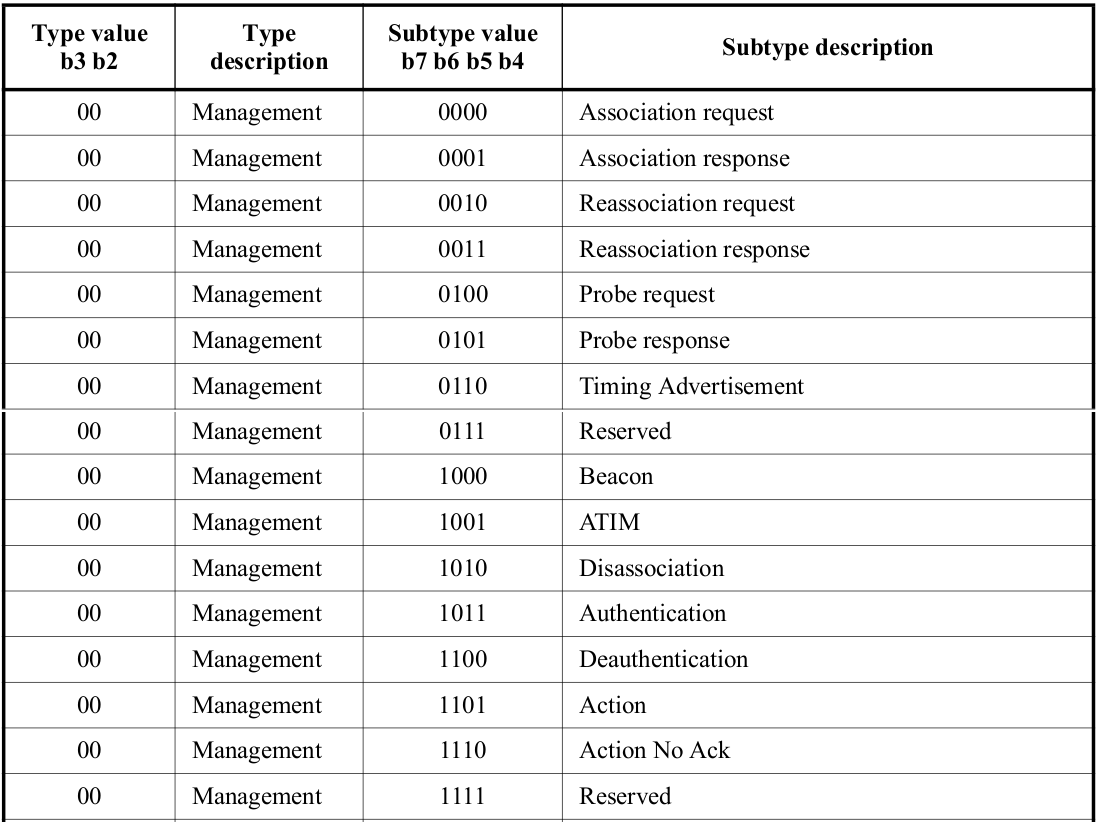
\includegraphics[width=\textwidth]{images/managementframes.png}
\end{table}

\subsection{Join}
Aus den entdeckten APs kann nun einer ausgewählt werden, um seinem Netzwerk (BSS) beizutreten \cite{ieee2012join}.
Es kann zwar geschehen, dass mehrere APs eines Netzwerks entdeckt wurden, eine Station kann jedoch zu jedem Zeitpunkt nur mit einem AP assoziert sein. \\
Um einem Netzwerk beizutreten muss sich die Station zunächst authentifizieren. 
Dieser Vorgang wird über einen \emph{Authentication Frame} (siehe Tabelle \ref{table:management}) initiiert \cite{ieee2012auth}. 
Das weitere Vorgehen hängt vom Authentifizierungsverfahren ab, zum Beispiel kann der AP einen verschlüsselten \emph{Challenge Text} an die Station senden, der mit einem aus dem Passwort erzeugten Schlüssel verschlüsselt wird und an den AP zurück gesendet werden kann. 
Ist die Antwort korrekt, bestätigt der AP den Vorgang mit einem \emph{Acknowledgement} und eventuell zusätzlichen Informationen für eine Stromchiffre. \\
Anschließend kann die Station mit dem AP assoziiert werden \cite{ieee2012associate}. 
Sie erhält nun eine IP und der AP gibt dem Netzwerk bekannt, dass er für die Station zuständig ist. 
Dies geschieht üblicherweise über das \emph{Address Resolution Protokoll} (ARP) oder das \emph{Internet Group Management Protocol} (IGMP).\\
Ist eine Station assoziert kann sie Datenverbindungen mit anderen Teilnehmern im Netzwerk aufbauen, sie könnte beispielweise das HTTP-Protokoll nutzen, um eine Webseite anzufordern.

\subsection{Reassociation}
Eine \emph{Reassoziation} wird durchgeführt, wenn die Station keine gute Verbindung mehr zu ihrem AP hat und ein AP des selben Netzwerks verfügbar ist, der eine bessere Verbindung bietet \cite{ieee2012reassociate}.
Um diesen neuen AP zu entdecken muss zunächst ein \emph{Scan} durchgeführt werden. \\
Anschließend sendet die Station einen \emph{Reassociation Request} an den neuen AP. 
Im \emph{Reassociation Request} wird der alte AP benannt, sodass der neue AP überprüfen kann, ob die Station tatsächlich mit ihm assoziert ist, gepufferte Pakete von ihm entgegennehmen und die Assoziation mit ihm auflösen kann.
Der Kommunikationsvorgang zwischen den APs wird auch als \emph{Handoff} bezeichnet. 
Wird dieser erfolgreich abgeschlossen antwortet der neue AP der Station mit einer \emph{Reassiciation Response}.
Abschließend wird dem Netzwerk die neue Assoziation mittels ARP mitgeteilt.


\section{Grundlagen der Bluetooth Spezifikation}
Bluetooth beschreibt eine Form der Funkkommunikation über kurze Distanzen, die zunächst für Mobiltelefone entwickelt und dann auf weitere Geräteklassen übertragen wurde.
Ursprünglich wurde die physische Schicht (PHY) und der Mediumszugriff (MAC) in der Spezifikation IEEE 802.15.1 definiert \cite{ieee2002blue}. 
Diese wird allerdings nicht mehr vom \emph{Institute of Electrical and Electronics Engineers} (IEEE) gepflegt. \\
Bluetooth ist bereits in der Version 5.0 erschienen, da jedoch zum Zeitpunkt der Recherche für diese Arbeit kaum kompatible Geräte wird im Folgenden auf Bluetooth 4.0 Bezug genommen \cite{blue2010spec}.
Bluetooth erlaubt es nach der Entdeckung eines Kommunikationspartners und anschließendem Aufbau einer Verbindung mit ihm im 2,4 GHz ISM-Band.
Die Reichweite für die Verbindung hängt neben äußeren Hindernissen und den verwendeten Antennen auch von der jeweiligen Sendeleistung ab.
Bluetooth Geräte werden dazu in drei Klassen eingeteilt, siehe Tabelle \ref{table:blclass}.

\begin{table}[h]
  \centering
	\caption{Klasseneinteilung für Bluetooth Geräte nach Sendeleistung, aus \cite{blue2010classes}.}
	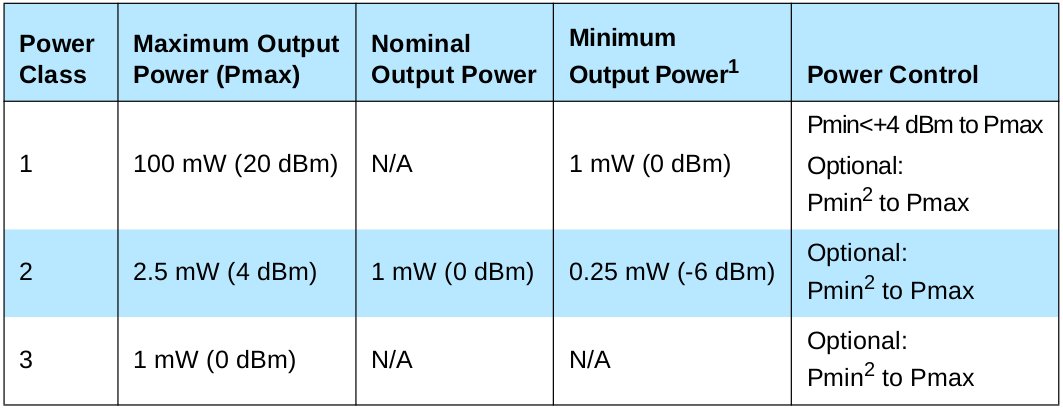
\includegraphics[width=0.9\textwidth]{images/blueclasses.png}
  \label{table:blclass}
\end{table}

Mit Bluetooth 4.0 wurde erstmals \emph{Bluetooth Low Energie} (BLE, auch Bluetooth Smart) vorgestellt.
BLE wurde für niedrigen Energieverbrauch optimiert, es verzichtet auf den Verbindungsaufbau, um den Zeitabschnitt in dem das Gerät aktiv ist zu reduzieren.
Da aber Informationen, die üblicherweise während des Verbindungsaufbaus übertragen werden, nun als \emph{Header} um das Datenpaket gepackt werden müssen, sinkt die Bruttodatenrate gegenüber Bluetooth deutlich \cite{rigado2016practical}. 
BLE eignet sich somit vor allem dann, wenn wenige oder selten Informationen ausgetauscht werden müssen.
Im Folgenden werden die, für die Lokalisation wichtigen Operationen vorgestellt.
Es handelt sich dabei jeweils um die Funktion des Entdeckens von Ressourcen mittels \emph{Inquiry Scan} für Bluetooth beziehungsweise mittels \emph{Advertising} für BLE.

\subsection{Inquiry Scan}
Eine Bluetooth-Verbindung besitzt immer einen \emph{Master} und einen \emph{Slave} \cite{blue2010inquiry}.
Da es sich beim \emph{Inquiry Scan} um eine Operation zum Entdecken von Ressourcen handelt ist, sind die Rollen noch nicht festgelegt. 
Die Spezifikation geht aber davon aus, dass der Sender der \emph{Inquiry Message} der \emph{Master} ist.
Nachdem der \emph{Master} die \emph{Inquiry Message} versendet hat antwortet der \emph{Slave} nach 625 $\mu$s mit einer \emph{Inquiry Response}. 
Soll eine erweiterte \emph{Inquiry Response} zum Einsatz kommen, wird dies in der \emph{Inquiry Response} gekennzeichnet und die erweiterte \emph{Inquiry Response} 1250 $\mu$s später gesendet.
Diese Zeiten sind den bei Bluetooth vorgesehenen Frequenzsprüngen angepasst.
Abbildung \ref{fig:inqscan} zeigt den Vorgang inklusive erweiterter \emph{Inquiry Response}.
Die Pakete sind entsprechend ihrer Inhaltsspezifikation benannt, \emph{ID} entspricht der \emph{Inquiry Message}, \emph{FHS} der \emph{Inquiry Response} und \emph{Extended Inquiry Response Packet} der erweiterten \emph{Inquiry Response}.

\begin{figure}[h]
  \centering
	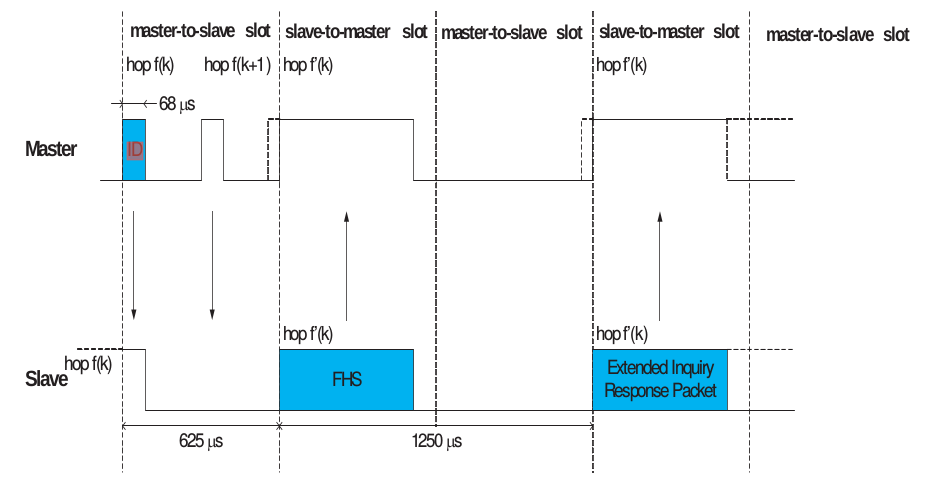
\includegraphics[width=\textwidth]{images/inqscan.png}
  \caption{\emph{Inquiry Scan} Vorgang, aus \cite{blue2010inquiry}.}
  \label{fig:inqscan}
\end{figure}

\subsection{Advertising}
Für das \emph{Advertising} stellt die Bluetooth Spezifikation drei über das Frequenzband verteilte Kanäle bereit \cite{blue2010channel}.
Auf diesen können BLE-Geräte \emph{Advertising Pakete} in einem unidirektionalen \emph{Broadcast} versenden.
\emph{Advertising} Pakete dürfen auch Nutzdaten enthalten, diese können dann von anderen, scannenden BLE-Geräten empfangen werden \cite{blue2010advertising}.
Allerdings dürfen die Nutzdaten maximal eine Länge von 31 Byte aufweisen \cite{blue2010pdu}.
Wurde zusätzlich im \emph{Advertising} Paket markiert, dass das Gerät verbindungsfähig ist, kann ein scannendes Gerät nach empfangen des \emph{Advertising} Paketes einen \emph{Scan Request} an das verbindungsfähige Gerät richten, um die Parameter für eine Verbindung auszuhandeln \cite{blue2010scanning}.

\section{Grundlagen von LoRa}
LoRa ist eine proprietäre Modulationstchnik und beschreibt somit eine physische Schicht.
LoRa ist für hohe Reichweite optimiert, bietet aber auch eine variable Sendeleistung, um den Energieverbrauch zu reduzieren.
LoRa beherrscht neben unterschiedlichen Frequenzen des ISM Bands, in Europa beispielsweise 433 und 868 MHz, auch eine adaptive Datenrate zwischen 0,3 und 50kbps.\\
Um den Mediumszugriff zu regeln wird die MAC-Schicht von LoRaWAN verwendet \cite{lora2015spec}.
LoRaWAN verwendet keine Kollisionsvermeidung, stattdessen dürfen Endgeräte zu jedem Zeitpunkt senden, solange sie dabei den Kanal zufällig wählen und die maximale Sendezeit beziehungsweise relative Frequenzbelegungsdauer nicht überschreiten.
Maximale Sendezeit und relative Frequenzbelegungsdauer werden dabei durch die länderspezifischen Regulierungsbehörden festgelegt.\\
LoRaWAN kann außerdem verwendet werden, wenn eine Verbindung nicht direkt zwischen zwei Kommunikationspartnern, sondern über ein \emph{Gateway} zustande kommen soll.
Dann muss diesem \emph{Gateway} zunächst beigetreten werden, danach können bestätige und unbestätigte Datenpakete über das \emph{Gateway} und ein dahinterliegendes Netzwerk ausgetauscht werden.
Tabelle \ref{table:mtype} zeigt die Nachrichtentypen von LoRaWAN.

\begin{table}[h]
  \centering
  \caption{Nachrichtentypen von LoRaWAN, aus \cite{lora2015spec}.}
	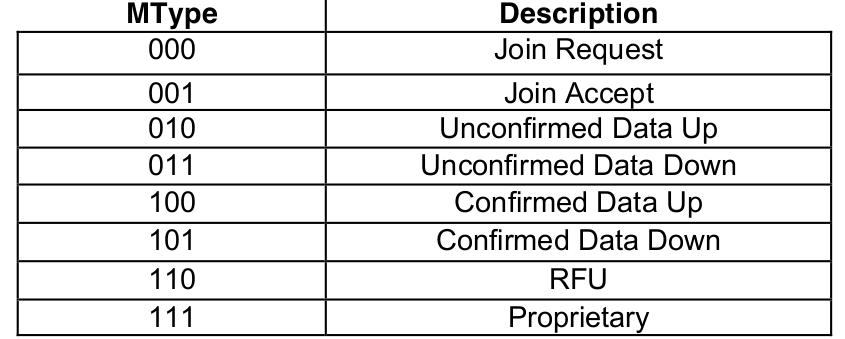
\includegraphics[width=0.8\textwidth]{images/mtype.png}
  \label{table:mtype}
\end{table}



\chapter{Analyse}
\label{ch:Analyse}
In diesem Kapitel werden zunächst einige verwandte Arbeiten vorgestellt und danach werden auf Basis dieser die Topologie, Protokolle und Messwerte für die Implementierungen dieser Arbeit ausgewählt.

\section{Verwandte Arbeiten} 
Die verwandten Arbeiten wurden in drei Unterkategorien unterteilt. 
Die erste Kategorie beschäftigt sich mit Selbstlokalisierung beziehungsweise indirekter Fernlokalisierung mittels 802.11.
Die Arbeiten der zweiten Kategorie basieren ebenfalls auf 802.11, hier wird jedoch eine Fernlokalisierung oder eine indirekte Selbstlokalisierung durchgeführt.
Die letzte Kategorie beschäftigt sich mit Arbeiten, die nicht auf 802.11 basieren, hier sind Verfahren beschrieben, die andere Protokolle verwenden.

\subsection{Verwandte Arbeiten - Selbstlokalisierung \& indirekte Fernlokalisierung mit 802.11}
Für die Selbstlokalisierung mit 802.11 werden auf der mobilen Einheit Messwerte für empfangene Pakete bestimmt und daraus die Position der mobilen Einheit berechnet.
Diese Information kann anschließend an einen Ortungsserver übertragen werden, dann handelt es sich um eine indirekte Fernlokaliserung.

\subsubsection{WiFi-LLS}
\label{ch:Vorherige:sec:LLS}
Chen et al. stellen mit dem WiFi-based Local Location System (WiFi-LLS) ein System zur indirekten Fernlokalisierung vor \cite{chen2007design}.
Als Messgröße wird die Stärke des empfangenen Signals (received signal strength, RSS) genutzt. 
Diese wird laut 802.11 Spezifikation als Index (RSSI) von der Hardware zurückgegeben. \\
Für die Ortung wird zunächst der RSSI von Paketen naher Access Points gemessen und zusammen mit der MAC-Adresse der mobilen Einheit in ein Paket gepackt und an den Ortungsserver versendet.
Anschließend wird auf dem Ortungsserver ein theoretisches Signalausbreitungsmodell $P(d) = P(d_0) - 10log_{10}(\frac{d}{d_0})^n - OAF$ mit der Distanz $d$, der Signalstärke $P(d)$ und der Referenzdistanz $d_0 = 1$m zur Bestimmung der Position der mobilen Einheit verwendet. \\
$P(d_0)$, der Pfadverlustexponent $n$ und der Hindernisdämpfungsfaktor $OAF$ müssen bestimmt werden, jedoch lassen sich $P(d_0)$ und $n$ auf einer einzelnen Teststrecke mit unterschiedlichen Abständen von AP und mobiler Einheit bestimmen. $OAF$ kann sogar für einen Gebäudetyp einmalig bestimmt werden.
Dadurch hat das Modell einen konstanten Aufwand. 
Dies ist für Baustellen interessant, da sich diese Werte einmalig messen und dann sogar über mehrere gleichartige Baustellen übertragen ließen.\\
In dieser Veröffentlichung steht die Ortungsgenauigkeit im Vordergrund und es werden keine Angaben zum Energieverbrauch gemacht. 
Als Referenz kann dienen, dass die mobile Einheit bei WiFi-LLS alle 5 Sekunden einen Scan (siehe Abschnitt \ref{ch:phase1:sec:scan}) durchführt, dann werden die Signalstärken entdeckter APs zusammen mit der eigenen MAC-Adresse in XML codiert und das so erzeugte Paket an den Ortungsserver versendet.

\subsubsection{AiRISTA Flow RTLS}
Ekahau bietet unter der Marke \textit{AiRISTA Flow RTLS} eine zu WiFi-LLS ähnliche Lösung kommerziell an \cite{airista2017airista}.
Ihr Ekahau B4 Badge Tag ermittelt regelmäßig den RSSI zu nahegelegenen APs und versendet diese an einen Ortungsserver \cite{liu2007survey}.
Das Tag bietet darüber hinaus noch einige Zusatzfunktionen, so können über die Datenverbindung auch Nachrichten und Alarmierungen an das Tag gesendet werden und die drei angebrachten Knöpfe können programmiert werden.\\
Bezüglich des Energieverbrauchs gibt sich das Informationsblatt des B4 Badge Tag vage: Das Tag soll abhängig vom Ortungsintervall wochenlang halten, danach muss der $600\ mA/h$ Akku geladen werden \cite{ekahau2017b4}.
Das Informationsblatt zum Ekahau W4, welches statt um den Hals am Handgelenk getragen wird, gibt an, dass der verbaute $530\ mA/h$ Akku bei einem Ortungsintervall von 15 Sekunden 500 Stunden (ca. 21 Tage) hält \cite{ekahau2017w4}.\\
AiRISTA Flow spricht auf ihrer Website zum Beispiel Krankenhäuser, Schulen und Regierungseinrichtungen an, hier sollen zusätzlich bewegliche Objekte, wie etwa Krankenhausbetten, geortet werden.
Die dazu verwendeten Asset Tags werden über einen Beschleunigungssensor aktiviert und können, wenn die Objekte selten bewegt werden, deutlich längere Laufzeiten erreichen \cite{ekahau2017a4}. \\
Im Umfeld des Tunnelbaus zeigte sich jedoch, dass die Tags keinesfalls wochenlange Laufzeiten aufwiesen, stattdessen entluden sie sich teilweise in unter zwölf Stunden.

\subsubsection{AeroScout}
Auch das AeroScout System von Stanley Healthcare richtet sich an den medizinischen Sektor und soll Objekte und Personen orten \cite{aeroscout2017asset}, \cite{aeroscout2017staff}.
Da sich auch dieses System in das bestehende WLAN-Netzwerk einfügt, sollte es ebenfalls auf einer indirekten Fernlokalisierung beruhen und demnach ähnliche Eigenschaften bezüglich des Energieverbrauchs aufweisen.\\
Das Informationsblatt ihres T14 Tags für Personen gibt eine Laufzeit von bis zu drei Wochen, abhängig von Konfiguration und Typ des Tags, an \cite{aeroscout2017t14}. 
Eine Angabe zu dem verwendeten Typ, der Konfiguration oder der Kapazität des verbauten Akkus wird nicht gemacht.\\

\subsubsection{Selbstlokalisierung mit Szenenanalyse}
\label{ch:Vorherige:sec:RSS-basierte}
Prasithsangaree et al. stellen ein System zur Selbstlokalisierung vor \cite{prasithsangaree2002indoor}, es verwendet aber eine offline-Phase zum Sammeln von Fingerabdrücken für Positionen in einem Abstand von 1,5 beziehungsweise 3 Metern. 
In diesen Fingerabdrücken werden die gemessenen RSSI der von den APs empfangenen Pakete als Merkmale zusammen mit der Position als Label gespeichert.
In der anschließenden online-Phase werden die gemessenen RSSI mit den Fingerabdrücken verglichen und die Position als gewichtetes Mittel der Labels bestimmt. \\
Die offline-Phase ist natürlich im Sinne der Aufgabenstellung nicht sinnvoll, da für eine Tunnelbreite von im Schnitt zehn Metern 4000 beziehungsweise 2000 Messungen pro Kilometer vorgenommen werden müssten.
Generell eignen sich Lösungen mit Szenenanalyse nicht gut für Baustellen, da diese nicht auf die potentiell höhere Genauigkeit angewiesen sind. 
Üblicherweise müssen dort sehr große Flächen vermessen werden und die Veränderungen durch den Baufortschritt führen dazu, dass regelmäßig neu gemessen werden muss.
Außerdem müssen bewegliche Störquellen wie Baumaschinen vorher aus dem Bereich entfernt werden, um unverfälschte Fingerabdrücke zu erhalten.
Der Aufwand ein System mit Szenenanalyse auf einer Baustelle zu betreiben ist deshalb sehr hoch und widerspricht der Forderung nach geringer Komplexität. \\
Die Arbeit zeigt aber die Volatilität der empfangenen Signalstärke auf, dies wurde 2011 von Lui et al. genauer untersucht \cite{lui2011differences}.
Lui et al. zeigen, dass die gemessene empfangene Signalstärke stark von der beteiligten Hardware abhängt und die Systeme jedes mal neu kalibriert werden müssen wenn sie auf ein neues AP-Modell portiert werden. 
Auf dem Areal sollte deshalb optimalerweise nur ein AP-Modell verwendet werden. \\
Abbildung \ref{fig:luiRSSI} zeigt die gemessenen RSSI Werte für die von ihnen getesten Netzwerkkarten mit unterschiedlichen Distanzen, für einige Karten korreliert die empfangene Signalstärke nur sehr schwach mit der Distanz zwischen Basisstation und mobiler Einheit.
Sie zeigen außerdem, dass einige AP-Modelle den RSSI speichern und nur bei größeren Veränderungen aktualisieren und dass die Antenne signifikanten Einfluss auf den protokollierten Wert hat.

\begin{figure}[h]
  \centering
	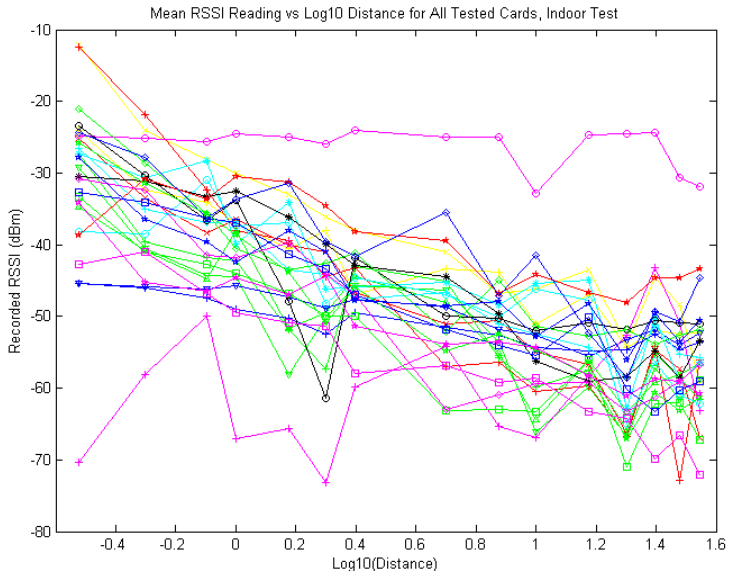
\includegraphics[width=\textwidth]{images/luiRSSI.png}
  \caption{Gemessener RSSI mit verschiedenen Access Points und Distanzen, aus \cite{lui2011differences}.}
  \label{fig:luiRSSI}
\end{figure}




\subsection{Verwandte Arbeiten - Fernlokalisierung \& indirekte Selbstlokalisierung mit 802.11}
Für die Fernlokalisierung mit 802.11 werden auf den Basisstationen Messwerte für empfangene Pakete bestimmt und daraus die Position der mobilen Einheit berechnet.
Diese Information kann anschließend an die mobile Einheit übertragen werden, dann handelt es sich um eine indirekte Selbstlokaliserung.

\subsubsection{RADAR}
\label{ch:Vorherige:sec:RADAR}
Das RADAR System von Bahl et al. (Microsoft Research) hat als eins der ersten WLAN-basierten Ortungssysteme viel Aufmerksamkeit erfahren \cite{bahl2000radar}.
Als Messgröße wird die Stärke des empfangenen Signals (received signal strength, RSS) genutzt, diese wird laut 802.11 Spezifikation als Index (RSSI) von der Hardware zurückgegeben. 
Das RADAR System ist auf eine offline-Phase angewiesen, in der empirisch ein Signalausbreitungsmodell aufgebaut wird. 
Es handelt sich also um ein System mit Szenenanalyse.\\
Die Verwendung einer offline-Phase ist im stark veränderlichen Baustellenumfeld nicht akzeptabel. 
Zum einen führt der ständige Baufortschritt dazu, dass regelmäßig neu kalibriert werden muss und zum anderen wirken sich auch die großen Baumaschinen auf die Signalausbreitung aus. 
Damit sich dies nicht im Modell wiederfindet, müssten zunächst alle beweglichen Maschinen aus dem Bereich entfernt werden, um anschließend in der online-Phase ihren Einfluss glätten zu können.
Die offline-Phase ist deshalb wirtschaftlich gesehen nicht durchführbar und das empirisch ermittelte Signalausbreitungsmodell müsste durch ein theoretisches ersetzt werden, für eine grobkörnige Bereichsortung sollte dies jedoch ausreichend sein.\\
Bei RADAR sendet die mobile Einheit vier UDP-Pakete pro Sekunde aus, an den Basisstationen wird dann der RSSI gemessen.
Die Autoren weisen jedoch darauf hin, dass sich dieser Vorgang leicht umkehren ließe, um von einer Fernlokalisierung auf eine Selbstlokalisierung zu kommen.
Bezüglich des Energieverbrauchs äußern sie sich jedoch zu keiner der beiden Varianten.\\
Die Position wird anschließend bestimmt, indem aus den in der offline-Phase aufgenommenen Werten derjenige mit dem geringsten Abstand zu den gemessen Werten gewählt wird. 
Dies wird im \textit{nearest neighbour in signal space (NNSS)} Algorithmus beschrieben.
Für die Ortung wird mehrfach gemessen und dann gemittelt, um im Median eine Genauigkeit von unter 3 Metern zu erhalten. 
Das kurze Sendeintervall von 0,25 Sekunden führt auch bei bewegten Personen zu einer Genauigkeit von 3,5 Metern.
Gleichzeitig sorgt das kurze Sendeintervall aber auch für einem hohen Energieverbrauch auf Seiten der mobilen Einheit, eine Reduktion der Sendevorgänge sollte im Kontext der Bereichsortung angestrebt werden, um den Energieverbrauch zu senken und die Batterielaufzeit der mobilen Einheit zu steigern.

\subsubsection{Verbesserungen an RADAR}
Bahl et al. veröffentlichten anschließend noch einige Verbesserungen für das ursprüngliche RADAR System \cite{bahl2000enhancements}.
Diese umfassen unter anderem den Einsatz von Access Points statt PCs als Basisstationen, verbesserte Ortung bewegter Personen und die Erkennung von hinzugekommenen Hindernissen wie etwa Personen.
Letzteres geschieht durch die Analyse der Signalstärke von Beacons anderer APs, da diese sich nicht bewegen, können Veränderungen in der Signalstärke als Veränderungen auf dem Signalweg gesehen werden.
Dies ließe sich auch auf größere Hindernisse übertragen, hängt aber stark von der strategischen Platzierung und möglichst dichten Verteilung der APs ab.\\
Auch hier äußern sich die Autoren nicht zum Energieverbrauch, wohl auch deshalb weil sie einen Laptop als mobile Einheit verwenden.

\subsubsection{Time-of-flight Lokalisierung}
\label{ch:Vorherige:sec:TOF}
Aufgrund der Schwächen von RSS-basierten Systemen wurde auch über solche nachgedacht, die stattdessen oder zusätzlich die time-of-flight (TOF) messen. 
Ein Beispiel für ein solches zeigen Wibowo et al. \cite{wibowo2009time}. 
Sie fordern optimalerweise Zugriff auf die physische Schicht (PHY) des 802.11 Protokolls, da auf diesen aber üblicherweise kein Zugriff besteht, messen sie TOF in der darüber liegenden MAC-Schicht.\\
Eine Basisstation sendet einen Beacon aus und protokolliert die Sendezeit, die mobile Einheit empfängt den Beacon, protokolliert die Empfangszeit und die Sendezeit der gesendeten Antwort, die Basisstation sichert die Empfangszeit der Antwort.
Nun sendet die mobile Einheit die zwei gespeicherten Zeitstempel an die Basisstation, der mit diesen die Verarbeitungszeit auf der mobilen Einheit berechnen kann, um dann die Distanz $d = c * (\frac{t_{empfangen} - t_{gesendet} - t_{Verarbeitung}}{2})$ zur mobilen Einheit zu bestimmen.
Dieses Schema lässt sich leicht von einer Fernlokalisierung in eine Selbstlokalisierung umwandeln, indem man den Initiator des Vorgangs tauscht.\\
Die Notwendigkeit die Zeitstempel bereits in der PHY- beziehungsweise MAC-Schicht zu setzen erfordert Zugriff auf die Software des als Basisstation verwendeten Access Points. 
Außerdem müssen die Zeitstempel im Bereich von Nanosekunden gesetzt werden und die Verarbeitungszeit vor/nach dem Setzen muss sehr konstant sein, da eine Abweichung von 100 ns bei c = 299.792.458 m/s bereits einen Fehler von 30 Metern verursacht.\\
Muthukrishnan et al. beschreiben diese Problematik bei dem Versuch TOF ohne Zugriff auf die Software des APs umzusetzen \cite{muthukrishnan2006using}.
Sie kommen zu dem Ergebnis, dass sich die in der Spezifikation eingebauten Zeitstempelfunktionen wie das Network Time Protocol (NTP), Ping und die Zeitstempel in Beacons nicht eignen, da sie zum einen nur eine Auflösung im Millisekundenbereich bieten und zum anderen von der Blockierungskontrolle von 802.11 (CSMA/CA) abhängen.

\subsubsection{Ortung ohne mobile Einheit}
Eine Ortung ohne mobile Einheit erfüllt wegen ihrer Abwesenheit offensichtlich jede Anforderung an die Batterielaufzeit der mobilen Einheit.
Mit MonoPHY stellen Abdel-Nasser et al. ein System zur Ortung ohne mobile Einheit vor \cite{abdel2013monophy}. \\
Dazu verwenden sie einen 802.11n-fähigen Laptop und Access Point und analysieren die Channel State Information (CSI) der physischen Schicht (PHY) der zwischen AP und Laptop übertragenen Daten.
Um die bestehende Struktur von APs zu nutzen, sollte das System angepasst und die CSI zwischen den APs gemessen werden.
Es hat jedoch einige Aspekte, die es ungeeignet für die Aufgabenstellung machen.\\
Das System unterscheidet nicht zwischen Personen, sondern erkennt nur, dass jemand anwesend ist. 
Außerdem ist es nur für eine Person in einem 100 $m^2$ Apartment gestaltet worden und müsste auf Baustellengröße und die Verfolgung vieler Personen erweitert werden.
Aber auch dann ist fraglich, wie gesichert werden kann, dass alle Personen durchgehend erkannt werden können, zum Beispiel wenn sich mehrere Personen auf oder in einem Transportfahrzeug aufhalten.
Auch ist es ohne Identifikation schwerer Fehler zu erkennen. 
Wird fälschlicherweise angezeigt, dass sich noch eine Peron im Tunnel befindet, kann oft durch ausrufen des Betreffenden festgestellt werden, dass dieser nicht im Tunnel ist. 
Hat man dagegen nur die Information, dass sich noch eine Person im Tunnel befindet, hat man keine Möglichkeit schnell herauszufinden ob dies der Wahrheit entspricht.\\
Weitere Probleme entstehen durch die Baumaschinen und Container. 
Diese haben einen starken Einfluss auf die CSI und verdecken dadurch möglicherweise nahe Personen und die Fahrzeugführer.
Deshalb müssten diese Objekte ebenfalls als Entitäten angezeigt werden. 
Die Anzeige diverser Kommandostände, Pausenräume und stehen gelassener Baumaschinen verwirrt im Notfall jedoch, da sich in jedem Objekt potentiell eine Person befinden könnte.\\
Die Veröffentlichung beruht außerdem auf der Verfügbarkeit der CSI, diese sind dort durch die Auswahl einer bestimmten Netzwerkkarte gegeben und sind nicht zwingend in einer bestehenden Struktur von APs verfügbar.
Als letzter Kritikpunkt steht die Verwendung eine offline-Phase, die, wie bereits diskutiert, wirtschaftlich nicht umsetzbar ist. \\ 
Somit erfüllt die Ortung ohne mobile Einheit zwar die Anforderungen an den Energieverbrauch, jedoch nicht die Forderung nach sicherer Erkennung von Abschnittswechseln, deshalb scheidet diese Technik zumindestens für Baustellen aus.




\subsection{Verwandte Arbeiten - Funkbasierte Lokalisierung ohne 802.11}
Die Arbeiten in dieser Kategorie verwenden nicht 802.11 für die Lokalisierung.
Sie verwenden stattdessen andere Protokolle, die sich durch einen geringeren Energieverbrauch als 802.11 auszeichnen sollen.

\subsubsection{Geeignete Messwerte für Bluetooth}
Hossain et al. untersuchen die laut Bluetooth Spezifikation zurückgegebenen Messwerte bezüglich ihrer Eignung für die Lokalisierung \cite{hossain2007comprehensive}.\\ 
Link Quality (LQ) beschreibt, wie gut die Verbindung zwischen zwei Geräten ist.
Der Wert wird aus der Bitfehlerrate beim Empfänger berechnet, allerdings ist nicht spezifiziert, wie der Wert zu berechnen ist, er hängt also in hohem Maße vom Hersteller des Empfängers ab. \\
Der Received Signal Strength Indicator (RSSI) misst die Stärke des eingehenden Signals, die Spezifikation sieht jedoch eine Golden Receive Power Range (GRPR) vor. 
Liegt der RSSI über oder unter dieser wird eine Anfrage zum erhöhen oder verringern der Sendeleistung an das andere Gerät verschickt, dies dient während einer aktiven Verbindung dazu den Energieverbrauch zu senken.
Problematisch am RSSI ist, dass er relativ zur GRPR bestimmt wird.
In der Untersuchung von Hossain et al. führte das dazu, dass der RSSI mit 0 gemessen wurde, wenn er innerhalb der GRPR lag. \\
Transmission Power Level (TPL) ist die Sendeleistung eines Geräts. 
TPL kann während einer bestehenden Verbindung durch Anfragen des Verbindungspartners verändert werden.
Dazu muss diese Energiesparfunktion jedoch unterstützt werden, was bei dem von Hossain et al. verwendeten Gerät nicht der Fall war.
Abbildung \ref{fig:bluetoothmess} zeigt deshalb für TPL eine waagerechte Linie.\\
Für Inquirys wird die Stärke des eingehenden Signals ohne die Beachtung des GRPR bestimmt.
Außerdem werden Inquirys immer mit voller Sendeleistung gesendet, da sie zur Entdeckung von Ressourcen verwendet werden.
Es handelt sich ebenfalls um den RSSI, um jedoch den Unterschied zum RSSI für eine Verbindung deutlich zu machen nennen Hossain et al. diesen Wert RX Power Level.

\begin{figure}[h]
  \centering
	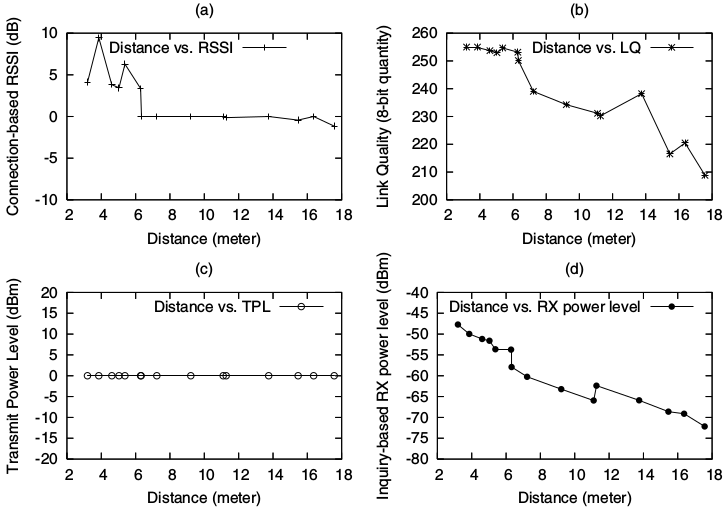
\includegraphics[width=\textwidth]{images/bluetoothmess.png}
  \caption{Korrelation der Messwerte mit der Distanz, aus \cite{hossain2007comprehensive}}
  \label{fig:bluetoothmess}
\end{figure}

\subsubsection{Antwortbasierte Inquiry Lokalisierung}
Bargh et al. stellen ein System zur Fernlokalisierung mittels Bluetooth Inquiry Scan vor \cite{bargh2008indoor}.
Die mobilen Einheiten sind dabei im discoverable ("{}entdeckbar"{}) Modus.
Die Basisstationen senden regelmäßig eine Inquiry Message aus, die dann von mobilen Einheiten in Reichweite mit einer Inquiry Response beantwortet werden. 
Anschließend werden die Antworten auf einem zentralen Ortungsserver gesammelt und die Positionen der mobilen Einheiten bestimmt.
Diese Information wird aus den beantworteten Inquiry Messages jeder mobilen Einheit gewonnen.
Dazu werden vorher in einer offline-Phase Fingerabdrücke für jeden Raum gesammelt.
In diesen wird gespeichert welche Inquiry Messages von der mobilen Einheit an einem bestimmten Ort beantwortet wurden.
Für die Bereichsortung entfiele diese offline-Phase, da der Bereich über die Beantwortung einer einzelnen Inquiry Message implizit bestimmt werden kann.
Tabelle \ref{table:irr} zeigt die abnehmende Warscheinlichkeit für eine Antwort auf die Inquiry Message mit steigender Distanz.

\begin{table}[h]
  \centering
  \caption{Rate der beantworteten Inquiry Messages (Inquiry Response Rate, IRR) gegen Distanz, aus \cite{bargh2008indoor}}
	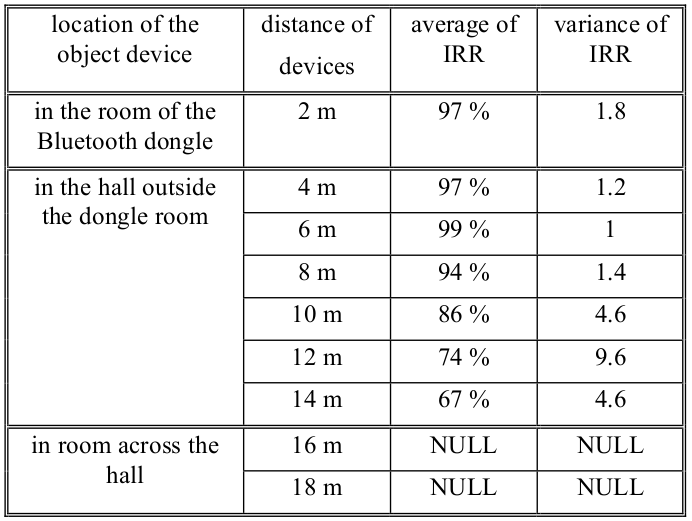
\includegraphics[width=0.7\textwidth]{images/irr.png}

  \label{table:irr}
\end{table}

\subsubsection{RSSI-basierte Inquiry Lokalisierung}
Ling et al. lokalisieren Bluetooth-fähige Geräte über den RSSI der Inquiry Response \cite{ling2010inquiry}.
Ihre Basisstationen versenden regelmäßig Inquiry Messages und messen den RSSI der Inquiry Responses.
Mobile Einheiten, die geortet werden wollen beziehungsweise sollen, bewerben in der Inquiry Response einen speziellen Service.
Dies erlaubt es diese herauszufiltern und die Privatsphäre anderer Personen zu wahren.
Die Autoren verwenden eine anfängliche offline-Phase um Fingerabdrücke für den RSSI an gegebenen zu finden.
Allerdings messen sie dazu an den Basisstationen die empfangene Signalstärke von Übertragungen anderer Basisstationen, folglich kann die offline-Phase automatisiert durchgeführt werden.
Für die online-Phase werden die gemessenen RSSI Werten über eine Warscheinlichkeitsverteilung geglättet, um eine bessere Ortungsgenauigkeit zu erreichen.
Für die eigentliche Lokalsierung werden die gemessenen RSSI mit den Warscheinlichkeitsverteilungen aus der offline-Phase verglichen und die Warscheinlichkeit für die Emission dieser Werte über die Position maximiert.

\subsubsection{RSSI-basierte BLE Lokalisierung}
Jianyong et al. stellen ein System zur Lokalisierung auf Basis von Bluetooth Low Energie (BLE, auch Bluetooth Smart) vor \cite{jianyong2014rssi}. \\
Sie messen an den Basisstationen den RSSI von Advertising Paketen, die zuvor von den mobilen Einheiten versendet wurden.
Für die genaue Ortung werden die Ergebnisse mit einem Gauß-Filter geglättet und für jede Basisstation die Parameter für ein Signalausbreitungsmodell bestimmt.
Die gemessene Signalstärke $P = A - 10n*log(d)$ hängt von der Referenzsignalstärke A im Abstand von einem Meter, dem Dämpfungsfaktor n und der Distanz d ab. \\
Jianyong et al. bestimmen die Referenzsignalstärke und den Dämpfungsfaktor für jede Basisstation.
Da jedoch nur eine Bereichsortung für diese Arbeit gefordert wurde, sollten A und n nur beispielhaft für eine Basisstation bestimmt werden, um den Aufwand beim Aufbau der Infrastruktur zu reduzieren.
Abbildung \ref{fig:blemodel} zeigt die von Jianyong et al. bestimmten Parameter für das Signalausbreitungsmodell. 
Abbildung \ref{fig:blemodel} zeigt außerdem, dass die verwendeten CC2540 Development Kit von Texas Instruments von einer Basisstation nur auf 20 Meter detektiert werden konnte.


\begin{figure}[h]
  \centering
	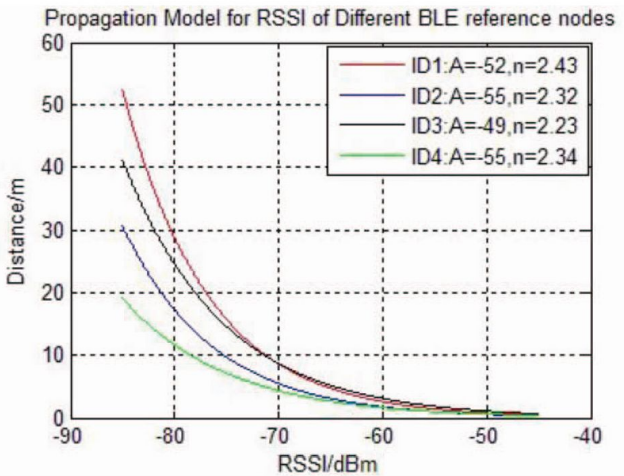
\includegraphics[width=0.7\textwidth]{images/blemodel.png}
  \caption{Signalausbreitungsmodelle aus \cite{jianyong2014rssi}}
  \label{fig:blemodel}
\end{figure}

\subsubsection{Lokalisierung mit LoRa}
Kim et al. stellen ein System zur Lokalisierung mit LoRa vor \cite{kim2016poster}.
Sie beziehen sich dabei auf eine Lokalisierung im Außenbereich in einem 30x30km Areal. 
Sie senden Pakete von der mobilen Einheit und messen die Time of Arrival (ToA) an den Basisstationen.
Dazu müssen die Basisstationen zeitsynchron arbeiten, dies wird über GPS sichergestellt.\\
Eine Lokalisierung über den RSSI lehnen sie ab, da dieser im Bereich von 20 bis 30km Entfernung nur um 3-6dBm fällt und die Varianz die Korrelation von RSSI und Distanz über lange Distanzen überdeckt.
Sie erreichen, abhängig von der Anzahl der verwendeten Basisstationen eien Genauigkeit zwischen wenigen Hundert und fast eintausend Metern, siehe dazu Abbildung \ref{fig:loraacc}

\begin{figure}[h]
  \centering
	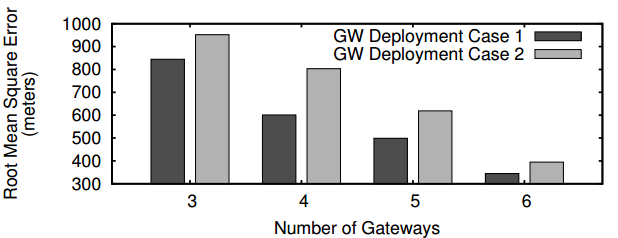
\includegraphics[width=0.7\textwidth]{images/loraacc.png}
  \caption{Quadratischer Fehler der Lokalisierung aus \cite{kim2016poster}, Gateways stellen Basisstationen dar.}
  \label{fig:loraacc}
\end{figure}


\section{Auswahl der Topologie}
Das Wissen um die Position der Nutzer soll nach der Ortung dem Sicherheitssystem der Baustelle zur Verfügung stehen. 
Das Sicherheitssystem fungiert daher konzeptionell auch als zentraler Ortungsserver.
Es muss deshalb eine Fernlokalisierung durchgeführt werden, diese kann aber sowohl direkt als auch indirekt durchgeführt werden. \\
Weil laut 802.11 keine für die Lokalisierung geeigneten Messwerte vom AP in das angeschlossene Netzwerk propagiert werden, kommt keine der verwandten Arbeiten zur direkten Fernlokalisierung ohne Zugriff auf die Software des AP aus.
In Abschnitt \ref{ch:Einleitung:sec:Zielsetzung} wurden sowohl Systeme ohne Änderungen der AP-Software als auch mit Änderungen dieser gefordert. \\
Diese Forderung lässt sich also in ein System zur indirekten Fernlokalisierung ohne Änderungen am AP und in ein System zur direkten Fernlokalisierung übersetzen.
Das System zur direkten Fernlokalisierung bedingt dabei Änderungen an der Software des AP, damit dieser den gewählten Messwert an den zentralen Ortungsserver übermittelt.\\
Dürfen Veränderungen der Hardware vorgenommen werden, bietet sich ebenfalls eine direkte Fernlokalisierung an, da dort die mobilen Einheiten, abgesehen von der Kollisionsdetektion/-vermeidung, nicht empfangen müssen.\\
Eine Topologie ohne Basisstationen kommt nicht in Frage, da diese Topologie Einzelpersonen insbesondere in Notsituationen nicht ausreichend gut erfasst.

\section{Auswahl des Funkprotokolls}
Soll das bestehende WLAN Netzwerk genutzt werden ist die Wahl auf die 802.11 Spezifikation beschränkt.\\
Für den dritten Schritt, der eine Änderung der verwendeten Hardware für die Basisstationen erlaubt, kann das Protokoll jedoch frei gewählt werden.
Bluetooth Low Energy wird gegenüber normalem Bluetooth aufgrund seiner Charakteristik als Protokoll für geringen Energieverbrauch bevorzugt.\\
LoRa bietet zwar theoretisch eine sehr hohe Reichweite, diese ist jedoch stark von verwendeten Antennen und den Hindernissen abhängig.
Ob LoRa einen signifikanten Vorteil bei der Reichweite hat muss geprüft werden.
Sollte dieser Vorteil bestehen, bietet LoRa durch seine bessere Abdeckung eine höhere Sicherheit bei der Erkennung von Abschnittswechseln. 
Außerdem ist es dadurch potentiell möglich auf triangulierte Positionen zu wechseln ohne mehr Basisstationen aufbauen zu müssen.


\section{Auswahl der Messwerte}
Da nur eine Bereichsortung durchgeführt werden soll, sind die Anforderungen an die Genauigkeit eines Messwertes gering.
Stattdessen sollte darauf geachtet werden, dass die Anforderung für die Messung gering ist.
Messwerte, die Zeitsynchronität vorraussetzen sind daher nicht geeignet.\\
Als Messwert wird der Received Signal Strength Index sowohl für WLAN als auch für Bluetooth Low Energy gewählt, da dieser bei jedem empfangenen Paket von der physischen Schicht gemessen und am empfangenden Gerät leicht ausgelesen werden kann.\\
Auch bei LoRa wird der RSSI gewählt. 
Da sich das Szenario im Gegensatz zu dem aus der Veröffentlichung von Kim et al. unter Tage abspielt kann keine Synchronisierung über GPS gewährleistet werden. 
Außerdem müssen die Distanzen zwischen den Basisstationen geringer gewählt werden, da die Ungenauigkeiten aus dieser Veröffentlichung zu hoch für das Szenario sind.

\chapter{Phase 1 - Keine Veränderungen an den APs}
\label{ch:phase1}
In einem ersten Schritt sollten laut Aufgabenstellung keine Veränderungen an den Access Points vorgenommen werden können.
Weil die Ortung deshalb auf WLAN basieren muss sind die Knoten im Folgenden immer APs. 
Ein Tag ist eine mobile Einheit, umgekehrt gilt dies jedoch nicht, da auch alle anderen WLAN-fähigen Geräte, wie Smartphones und Laptops, eine mobile Einheit sein kommen. \\
Die Unveränderlichkeit bedeutet insbesondere auch, dass keine Messwerte verwendet werden können, die direkt am AP gemessen werden müssen und nicht als Teil der 802.11 in das dahinterliegende Netzwerk weitergeleitet werden.
Da time of arrival Synchronisation und präzise Timer bei den APs vorraussetzt und time difference of arrival nur von den APs gemessen werden kann, eignen sich diese Messgrößen nicht für diese Aufgabenstellung.
Received signal strength und roundtrip time of flight können auf der mobilen Einheit gemessen werden, nicht jedoch an den APs, da die in der PHY- beziehungsweise MAC-Schicht gemessenen Werte nicht an weitere Empfänger im Netzwerk propagiert werden. 
Somit scheidet die direkte Fernlokalisierung mangels Messgrößen aus, es wird stattdessen eine indirekte Fernlokalisierung durchgeführt bei der die mobile Einheit eine Selbstlokalisierung durchführt und das Ergebnis dem Ortungsserver über eine Datenverbindung mitteilt.


\section{Vorherige Arbeiten}
\label{ch:phase1:sec:vorherige}
Zunächst werden vorherige Arbeiten behandelt, es werden sowohl wissenschaftliche als auch kommerzielle Lösungen betrachtet.


\subsection{WiFi-LLS}
\label{ch:Vorherige:sec:LLS}
Chen et al. stellen mit dem WiFi-based Local Location System (WiFi-LLS) ein System zur indirekten Fernlokalisierung vor \cite{chen2007design}.
Als Messgröße wird die Stärke des empfangenen Signals (received signal strength, RSS) genutzt, diese wird laut 802.11 Spezifikation als Index (RSSI) von der Hardware zurückgegeben. \\
Für die Ortung wird zunächst der RSSI von Paketen naher APs gemessen und zusammen mit der MAC-Adresse der mobilen Einheit in ein Paket gepackt und an den Ortungsserver versendet.
Anschließend wird auf dem Ortungsserver ein theoretisches Signalausbreitungsmodell $P(d) = P(d_0) - 10log_{10}(\frac{d}{d_0})^n - OAF$ mit der Distanz $d$, der Signalstärke $P(d)$ und der Referenzdistanz $d_0 = 1m$ zur Bestimmung der Position der mobilen Einheit verwendet. \\
$P(d_0)$, der Pfadverlustexponent $n$ und der Hindernisdämpfungsfaktor $OAF$ müssen bestimmt werden, jedoch lassen sich $P(d_0)$ und $n$ auf einer einzelnen Teststrecke mit unterschiedlichen Abständen von AP und mobiler Einheit bestimmen. $OAF$ kann sogar für einen Gebäudetyp einmalig bestimmt werden.
Dadurch hat das Modell einen konstanten Aufwand. 
Dies ist für Baustellen interessant, da sich diese Werte einmalig messen und dann sogar über mehrere gleichartige Baustellen übertragen ließen.\\
In dieser Veröffentlichung steht die Ortungsgenauigkeit im Vordergrund und es werden keine Angaben zum Energieverbrauch gemacht. 
Als Referenz kann dienen, dass die mobile Einheit bei WiFi-LLS alle 5 Sekunden einen Scan (siehe Abschnitt \ref{ch:phase1:sec:scan}) durchführt, dann werden die Signalstärken entdeckten APs zusammen mit der eigenen MAC-Adresse in XML codiert und das so erzeugte Paket an den Ortungsserver versendet.

\subsection{AiRISTA Flow RTLS}
Ekahau bietet unter der Marke \textit{AiRISTA Flow RTLS} eine, zu WiFi-LLS ähnliche, Lösung kommerziell an \cite{airista2017airista}.
Ihr Ekahau B4 Badge Tag ermittelt regelmäßig den RSSI zu nahegelegenen Access Points und versendet diese an einen Ortungsserver \cite{liu2007survey}.
Das Tag bietet darüber hinaus noch einige Zusatzfunktionen, so können über die Datenverbindung auch Nachrichten und Alarmierungen an das Tag gesendet werden und die drei angebrachten Knöpfe können programmiert werden.\\
Bezüglich des Energieverbrauchs gibt sich das Informationsblatt des B4 Badge Tag vage: Das Tag soll abhängig vom Ortungsintervall wochenlang halten, danach muss der $600\ mA/h$ Akku geladen werden \cite{ekahau2017b4}.
Das Informationsblatt zum Ekahau W4, welches statt um den Hals am Handgelenk getragen wird, gibt an, dass der verbaute $530\ mA/h$ Akku bei einem Ortungsintervall von 15 Sekunden 500 Stunden (ca. 21 Tage) hält \cite{ekahau2017w4}.\\
AiRISTA Flow spricht auf ihrer Website zum Beispiel Krankenhäuser, Schulen und Regierungseinrichtungen an, hier sollen zusätzlich bewegliche Objekte, wie etwa Krankenhausbetten, geortet werden.
Die dazu verwendeten Asset Tags werden über einen Beschleunigungssensor aktiviert und können, wenn die Objekte selten bewegt werden, deutlich längere Laufzeiten erreichen \cite{ekahau2017a4}. \\

\subsection{AeroScout}
Auch das AeroScout System von Stanley Healthcare richtet sich an den medizinischen Sektor und soll Objekte und Personen orten \cite{aeroscout2017asset}, \cite{aeroscout2017staff}.
Da sich auch dieses System in das bestehende WLAN-Netzwerk einfügt, sollte es ebenfalls auf einer indirekten Fernlokalisierung beruhen und demnach ähnliche Eigenschaften bezüglich des Energieverbrauchs aufweisen.\\
Das Informationsblatt ihres T14 Tags für Personen gibt eine Laufzeit von bis zu drei Wochen, abhängig von Konfiguration und Typ des Tags, an \cite{aeroscout2017t14}. 
Eine Angabe zu dem verwendeten Typ, der Konfiguration oder der Kapazität des verbauten Akkus wird nicht gemacht.\\

\subsection{Selbstlokalisierung mit Szenenanalyse}
\label{ch:Vorherige:sec:RSS-basierte}
Prasithsangaree et al. stellen ein System zur Selbstlokalisierung vor \cite{prasithsangaree2002indoor}, es verwendet aber eine offline-Phase zum Sammeln von Fingerabdrücken für Positionen in einem Abstand von 1,5 beziehungsweise 3 Metern. 
In diesen Fingerabdrücken werden die gemessenen RSSI der von den APs empfangenen Pakete als Merkmale zusammen mit der Position als Label gespeichert.
In der anschließenden online-Phase werden die gemessenen RSSI mit den Fingerabdrücken verglichen und die Position als gewichtetes Mittel der Labels bestimmt. \\
Die offline-Phase ist natürlich im Sinne der Aufgabenstellung nicht sinnvoll, da für eine Tunnelbreite von 10m 4000 beziehungsweise 2000 Messungen pro Kilometer vorgenommen werden müssten.
Generell eignen sich Lösungen mit Szenenanalyse nicht gut für Baustellen, da diese nicht auf die potentiell höhere Genauigkeit angewiesen sind. 
Üblicherweise müssen dort sehr große Flächen vermessen werden und die Veränderungen durch den Baufortschritt führen dazu, dass regelmäßig neu gemessen werden muss.
Außerdem müssen bewegliche Störquellen wie Baumaschinen vorher aus dem Bereich entfernt werden, um unverfälschte Fingerabdrücke zu erhalten.
Der Aufwand ein System mit Szenenanalyse auf einer Baustelle zu betreiben ist deshalb sehr hoch und widerspricht der Forderung nach geringer Komplexität. \\
Die Arbeit zeigt aber die Volatilität der empfangenen Signalstärke auf, dies wurde 2011 von Lui et al. genauer untersucht \cite{lui2011differences}.
Lui et al. zeigen, dass die gemessene empfangene Signalstärke stark von der beteiligten Hardware abhängt und die Systeme jedes mal neu kalibriert werden müssen wenn sie auf ein neues AP-Modell portiert werden. 
Auf dem Areal sollte deshalb optimalerweise nur ein AP-Modell verwendet werden. \\
Abb. \ref{fig:luiRSSI} zeigt die gemessenen RSSI Werte für die von ihnen getesten Netzwerkkarten mit unterschiedlichen Distanzen, für einige Karten korreliert die empfangene Signalstärke nur sehr schwach mit der Distanz zwischen Knoten und mobiler Einheit.
Sie zeigen außerdem, dass einige AP-Modelle den RSSI speichern und nur bei größeren Veränderungen aktualisieren und dass die Antenne signifikanten Einfluss auf den protokollierten Wert hat.



\begin{figure}[h]
  \centering
	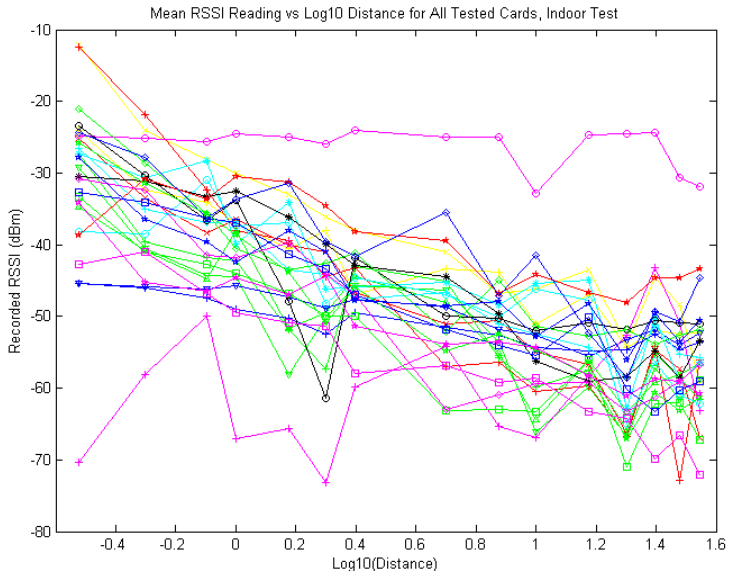
\includegraphics[width=\textwidth]{images/luiRSSI.png}
  \caption{Gemessener RSSI mit verschiedenen Access Points und Distanzen, aus \cite{lui2011differences}.}
  \label{fig:luiRSSI}
\end{figure}

\section{Grundlagen der 802.11 Spezifikation}
\label{ch:phase1:sec:grundlagen}
802.11 beschreibt eine Form der drahtlosen Datenübertragung mittels Funkwellen \cite{ieee2012macphy}.
Die Spezifikation beschreibt die physische Schicht (PHY-Layer) und den Mediumszugriff (MAC-Layer) für ein Funknetzwerk, dass sich mit den darüber liegenden Schichten des OSI-Modells in andere Netzwerke eingebunden werden kann.
Wird ein solches Netzwerk in ein Local Area Network (LAN) eingebunden spricht man üblicherweise vom Wireless Local Area Network (WLAN).
Die 1997 erstmals verabschiedete Spezifikation wurde häufig erweitert und wird in ihrer ursprünglichen Form praktisch nicht mehr angewendet, da die Datenraten zu gering sind.
Die Erweiterungen werden mit Buchstaben benannt (zum Beispiel 802.11g) und verändern entwa die verwendete Frequenz und Modulationsverfahren.\\
Zur Vermeidung von Kollisionen kommt Carrier Sense Multiple Access/Collision Avoidance (CSMA/CA) zum Einsatz.
Bei CSMA/CA wird zunächst das Medium belauscht und gewartet bis keine Signale mehr auf dem Medium sind. 
Dann muss ein Inter Frame Spacing (IFS) abgewartet werden, je nach Priorität ist dieses unterschiedlich lang (SIFS<PIFS<DIFS<EIFS), anschließend kann gesendet werden.
Tritt trotzdem eine Kollision auf, versucht der Sender es erneut mit einem längeren IFS.\\
802.11 spezifiziert ebenfalls mehrere Operationen, die beispielsweise zur Entdeckung von Ressourcen und der Authentifizierung an einer Ressource dienen, einige, für diese Arbeit wichtige Operationen werden im Folgenden beschrieben.

\subsection{Scan}
\label{ch:phase1:sec:scan}
Scan ist eine Operation zur Entdeckung von Access Points, sie kann von einer Station (Endverbraucher, zum Beispiel Smartphone oder Laptop) aktiv oder passiv ausgeführt werden \cite{ieee2012scan}.
Bei einem passiven Scan empfängt die Station und filtert die von Access Points regelmäßig gesendeten Beacons heraus, diese gelten dann als entdeckt.
Ein Beacon Frame ist ein Management Frame, der dazu gedacht ist, technische Möglichkeiten des APs zu bewerben, zum Beispiel die möglichen Datenraten und Zeitstempel zur Synchronisierung.
Versteckte APs senden keine Beacons. \\
Bei einem aktiven Scan sendet die Station einen Probe Request aus, dieser kann sowohl an alle APs (broadcast) als auch an einen speziellen AP adressiert sein.
Ein Probe Requests bewirbt, ähnlich wie ein Beacon, die technischen Möglichkeiten der Station.
Der addressierte AP, beziehungsweise im Falle des broadcasts alle APs, beantwortet den Probe Request mit einer Probe Response in der er mitteilt welche der beworbenen Funktionen er ebenfalls unterstützt, die Station schließt den Vorgang mit einem Acknowlegement ab. \\
Das 2,4GHz ISM-Band wird in Europa in 13 je 10MHz breite Kanäle aufgeteilt, da ein AP immer nur auf einem Kanal aktiv ist müsste jeder Kanal gescannt werden.
Praktisch werden jedoch breitere Kanäle verwendet, 802.11g verwendet beispielsweise 20MHz breite Kanäle, so dass effektiv nur die Kanäle 1, 5, 9 und 13 geprüft werden müssen. \\
Tabelle \ref{table:management} listet alle in der 802.11 Spezifikation gelisteten Management Frames.
Ein Management Frame wird durch die Typenbits markiert und durch die Bits für den Subtypen weiter unterschieden.

\begin{table}[h]
	\centering
	\caption{Management Frames nach 802.11 \cite{ieee2012management}}
	\label{table:management}
	\begin{tabular}{l|l|l}
		Type & Subtype & Beschreibung \\
		\hline
		00 & 0000 & Association Request  \\
		00 & 0001 & Association Response  \\
		00 & 0010 & Reassociation Request  \\
		00 & 0011 & Reassociation Response  \\
		00 & 0100 & Probe Request  \\
		00 & 0101 & Probe Response  \\
		00 & 0110 & Timing Advertisement  \\
		00 & 0111 & Reserved  \\
		00 & 1000 & Beacon  \\
		00 & 1001 & ATIM  \\
		00 & 1010 & Disassociation  \\
		00 & 1011 & Authentification  \\
		00 & 1100 & Deauthentification  \\
		00 & 1101 & Action  \\
		00 & 1110 & Action No Ack  \\
		00 & 1111 & Reserved  \\
	\end{tabular}
\end{table}

\subsection{Join}
Aus den entdeckten APs kann nun einer ausgewählt werden um seinem Netzwerk (BSS) beizutreten \cite{ieee2012join}.
Es kann zwar geschehen, dass mehrere APs eines Netzwerks entdeckt wurden, eine Statíon kann jedoch zu jedem Zeitpunkt nur mit einem AP assoziert sein. \\
Um einem Netzwerk beizutreten muss sich die Station zunächst authentifizieren, dieser Vorgang wird über einen Authentication Frame (siehe Tabelle \ref{table:management}) initiiert \cite{ieee2012auth}. 
Das weitere Vorgehen hängt vom Authentifizierungsverfahren ab, zum Beispiel kann der AP einen verschlüsselten Challenge Text an die Station senden, der mit einem aus dem Passwort erzeugten Schlüssel entschlüsselt wird und an den AP zurück gesendet werden kann. 
Ist die Antwort korrekt bestätigt der AP den Vorgang mit einem Acknowledgement und eventuell zusätzlichen Informationen für eine Stromchiffre. \\
Anschließend kann die Station mit dem AP assoziiert werden \cite{ieee2012associate}. 
Sie erhält nun eine IP und der AP gibt dem Netzwerk bekannt, dass er für die Station zuständig ist, dies geschiet  üblicherweise über das Address Resolution Protokoll (ARP). [evtl IGMP?] \\
Ist eine Station assoziert kann sie Datenverbindungen mit anderen Teilnehmern im Netzwerk aufbauen, sie könnte beispielweise das HTTP-Protokoll nutzen um eine Webseite anzufordern.

\subsection{Reassociation}
Eine Reassociation wird durchgeführt wenn die Station keine gute Verbindung mehr zu ihrem AP hat und ein AP des selben Netzwerks verfügbar ist, der eine bessere Verbindung bietet \cite{ieee2012reassociate}.
Um diesen neuen AP zu entdecken muss zunächst ein Scan durchgeführt werden. \\
Anschließend sendet die Station einen Reassociation Request an den neuen AP, im Reassociation Request wird der alte AP benannt, so dass der neue AP überprüfen kann, ob die Station tatsächlich mit ihm assoziert ist, gepufferte Pakete von ihm entgegennehmen und die Assoziation mit ihm auflösen kann.
Der Kommunikationsvorgang zwischen den APs wird auch als Handoff bezeichnet, wird dieser erfolgreich abgeschlossen antwortet der neue AP der Station mit einer Reassiciation Response.
Abschließend wird dem Netzwerk die neue Assoziation mittels ARP mitgeteilt.

\begin{figure}[h]
  \centering
	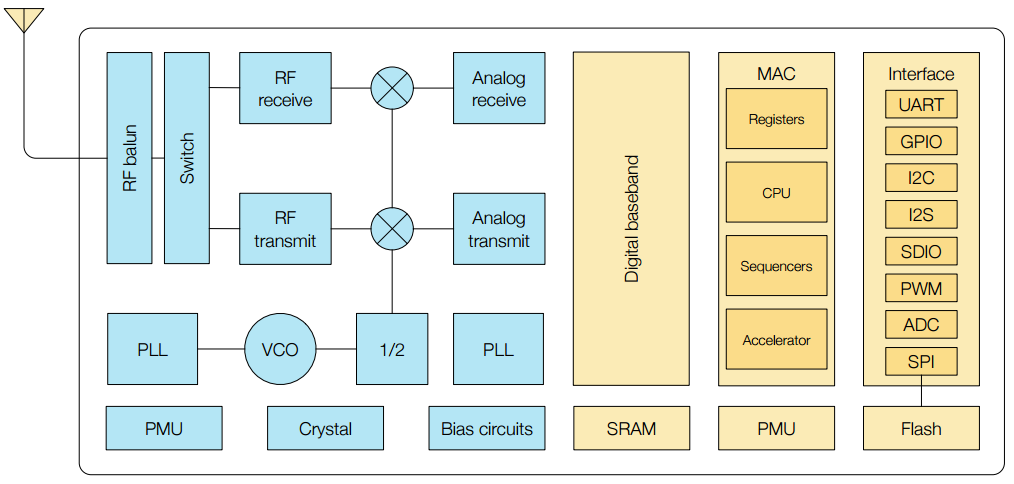
\includegraphics[width=\textwidth]{images/espblock.png}
  \caption{Blockdiagramm des ESP8266, aus \cite{espressif2017esp8266}}
  \label{fig:espblock}
\end{figure}

\section{ESP8266}
Der ESP8266 soll als Hardware für das Tag eingesetzt werden, dabei handelt es sich um einen Microcontroller von Espressif.
Der Esp8266 besitzt neben einer CPU eine 802.11b/g/n"-/e/i-fähige WLAN-Einheit und diverse andere, kabelgebundene Kommunikationsstandards wie zum Beispiel GPIO, I2C und SPI, siehe Abb. \ref{fig:espblock}. \\
Da der ESP8266 selbst weder über Flashspeicher, noch über eine Antenne verfügt wird er auf einem Modul mit diesen Komponenten verbaut, die in dieser Arbeit betrachteten Module sind das ESP12-S und das ESP12-F.
Das neuere ESP12-F sollte eine höhere Reichweite bei der Funkübertragung entfalten, dies wird noch Gegenstand eines Experiments sein.
Abb. \ref{fig:espmodules} zeigt die beiden Module nebeneinander, die unterschiedlichen Antennenformen sind deutlich zu erkennen.\\
Espressif gibt im Datenblatt auch Aufschluss über den Energieverbrauch des ESPs, siehe dazu Abb. \ref{fig:esppower}.
Für die Prototypenentwicklung wird ein ESP12-S Modul auf einem Adafruit Feather Huzzah verwendet, dieses stellt mit dem CP2104 eine serielle Schnittstelle zum ESP her, reguliert die Spannung für das Modul auf 3,3V und bringt den 2mm Pinabstand des ESP12-S Moduls auf die für Breadboards üblichen 2,5mm.
Das Adafruit Feather Huzzah mit ESP12-S ist in Abb. \ref{fig:espmodules} links abgebildet.

\begin{figure}[h]
  \centering
	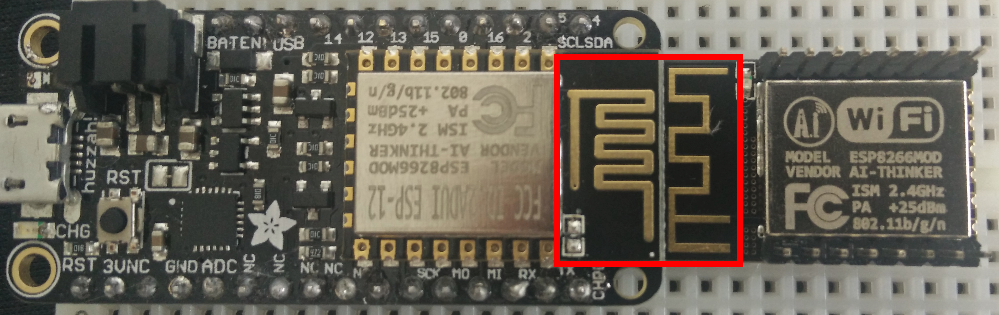
\includegraphics[width=\textwidth]{images/espmodules.png}
  \caption{Vergleich der Antennen, links: ESP12-S verbaut auf einem Adafruit Feather Huzzah, rechts: ESP12-F}
  \label{fig:espmodules}
\end{figure}

\begin{figure}[h]
  \centering
	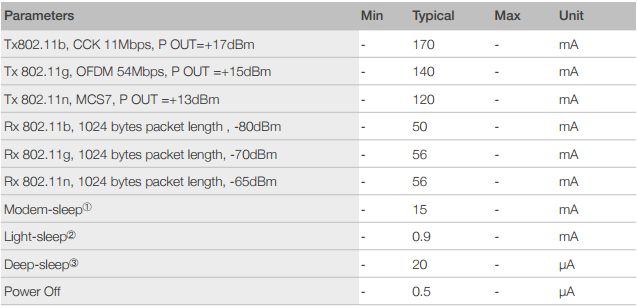
\includegraphics[width=\textwidth]{images/esppower.png}
  \caption{Energieverbrauch des ESP8266 bei verschiedenen Operationen, aus \cite{espressif2017esp8266}}
  \label{fig:esppower}
\end{figure}


\subsection{ESP8266 Arduino Core}
Eine einfache Möglichkeit den ESP8266 zu programmieren stellt die bekannte Arduino IDE dar \cite{banzi2017arduino}.\\
Unter Windows muss zunächst der Treiber für den \textit{CP2104 USB-to-Serial Chip} installiert werden, auf Linux und Mac entfällt dieser Schritt \cite{fried2017feather}.
Nach der Installation der Arduino IDE muss dort in den Einstellungen unter \textit{Additional Boards Manager URLs} die URL \url{http://arduino.esp8266.com/stable/package_esp8266com_index.json} hinzugefügt werden.  
Nach einem Neustart der IDE kann im \textit{Boards Manager} das Paket für den ESP8266 heruntergeladen werden und anschließend das Board \textit{Adafruit HUZZAH ESP8266} ausgewählt werden. \\
Ist das Board über USB mit dem Computer verbunden kann nun eigener Code oder eines der Beispiele aus \textit{Examples for Adafruit HUZZAH ESP8266} mit STRG+U auf den ESP geladen werden. 
Dieser Vorgang wird im Folgenden als flashen bezeichnet. \\
Der ESP8266 Arduino Core wird als Open Source Projekt gepflegt und setzt die ESP Open SDK auf einen, für die Arduino IDE üblichen Stil um \cite{arduino2017core}. 
Dabei wird möglichst die Kompatibilität zu Arduino gewahrt, das führt oft dazu, dass bereitgestellte Funktionen der SDK nicht in Arduino umgesetzt wurden.
Sollten die Funktionen dennoch benötigt werden können die Header-Dateien der SDK direkt importiert werden:

\begin{verbatim}
//Hier wird ein Header des ESP8266 Arduino Core importiert
#include <ESP8266WiFi.h> 

//Hier wird ein Header der ESP Open SDK importiert
extern "C" {#include "user_interface.h"} 
\end{verbatim}

Der ESP8266 Arduino Core wurde in der Version 2.3.0 verwendet.

\subsection{ESP Open SDK}
Statt mit der Arduino Core Umsetzung der ESP Open SDK kann natürlich auch direkt mit ihr programmiert werden \cite{esp2017open}. \\
Dazu muss zunächst das Github Projekt geklont werden: \texttt{git clone --recursive \url{https://github.com/pfalcon/esp-open-sdk}.git} und anschließend mit \texttt{make} kompiliert werden.
Wurde die Kompilierung erfolgreich abgeschlossen sollte die Pfadvariable (PATH) entsprechend der Meldung des make-Tools erweitert werden. \\
Die in C geschriebenen Programme können nun mit einem modifizierten GCC-Kompiler kompiliert und anschließend mit dem esptool.py zunächst in ein Image umgewandelt und dann geflasht werden. 
Das in \textit{examples} enthaltene \textit{blinky} Beispiel beinhaltet neben dem Beispielcode eine Makefile, in der diese Schritte nachvollzogen werden können, mit \texttt{make flash} wird das Beispiel kompiliert und geflasht. \\
Programme werden in regulärem C unter Zuhilfenahme der in \texttt{/sdk/include} enthaltenen Header-Dateien geschrieben, zu beachten ist nur, dass einige Funktionen der \texttt{stdlib.h} nicht verwendet werden können.
Dies betrifft vor allem direkten Speicherzugriff wie zum Beispiel \texttt{memcpy}, hier muss stattdessen \texttt{os\_memcpy} verwendet werden.
Alle betroffenen Funktionen sind in \texttt{osapi.h} beschrieben. \\
Einige frühe Experimente zeigten, dass Programme, die mit der ESP Open SDK geschrieben wurden auf dem ESP schneller starten als solche, die mit dem ESP8266 Arduino Core geschrieben wurden.
Diese Andeutung von Ineffizienzen bei der Übersetzung von Arduino Code wurde zum Anlass genommen, für die nachfolgenden Implementierungen nach der Fertigstellung des Prototypen in Arduino ebenfalls eine Implementierung in C hinzuzufügen, um ein optimales Programm zu erhalten. \\
Die ESP Open SDK wurde in der Version 2.0.0 verwendet.



\section{WiFi-LSS Implementierung}
Die mobile Einheit des WiFi-LLS Systems führt alle 5 Sekunden einen Scan aus, kodiert die Ergebnisse in XML und versendet sie an den Ortungsserver \cite{chen2007design}.
Da der Fokus dieser Arbeit auf dem Energieverbrauch liegt werden für die Referenzimplementierung eines WiFi-LLS-Tags die Kodierung in XML durch eine simple String Kodierung ersetzt und die Ergebnisse werden über UDP an den Ortungsserver übermittelt. 
Damit wird der overhead einer TCP-Verbindung vermieden.\\
Zunächst muss sich das Tag dem Netzwerk beitreten (Join) und anschließend einen Scan ausführen und ein UDP-Paket versenden.
Da die Scan-Funktion des ESP8266 Arduino Core es nicht erlaubt den RSSI zu einem AP auszulesen muss \texttt{user\_interface.h} importiert und die Scan-Funktion der SDK direkt verwendet werden.
Um den Energieverbrauch weiter zu reduzieren, soll der ESP möglichst viel Zeit in Energiesparzuständen verbringen.
Der tiefste Schlafzustand, der dennoch eine Aufrechterhaltung der WLAN-Verbindung erlaubt ist der \texttt{light\_sleep}. 
Er wird vom ESP automatisch aufgerufen, wenn er keine Aufgaben zu erledigen hat.
Er kann aber auch manuell aufgerufen werden, beides wurde getestet.\\
Einige Parameter können gewählt werden: Insbesondere die Intervallzeit bestimmt, wie oft der ESP aktiv ist und damit auch wie viel Energie er verbraucht.
Für Mitarbeiter im Tunnel kann von einer Maximalgeschwindigkeit von $30\ km/h$ ausgegangen werden, diese wird durch Schienen- oder Lastkraftfahrzeuge erreicht. 
Die maximale Reichweite des ESP12-S beziehungsweise ESP12-F Moduls ist nicht bekannt und muss noch bestimmt werden, sie wird zwischen 50 und 100 Metern angenommen.
Es wurde daher ein Intervall von 5 Sekunden gewählt, in dieser Zeit bewegt sich ein Mitarbeiter bei $30\ km/h$ ca. $42\ m$.\\
Des Weiteren kann theoretisch die Zahl der gescannten Kanäle gewählt werden, da sich die Einflussbereiche der APs in einem WLAN-Netzwerk üblicherweise überlappen ist es aber sinnvoll diese über die 4 nichtüberlappenden Kanäle zu verteilen. 
Eine Implementierung die nur einen Kanal scannt tritt deshalb nur außer Konkurenz an.\\
Tabelle \ref{table:llsconsumption} zeigt den gemessen Energieverbrauch der Implementierungen in Arduino und C, jeweils mit und ohne manuell aufgerufenen \texttt{light\_sleep} und eine Implementierung, die nur einen Channel scannt.
Für die Tests wurde das Adafruit Feather Huzzah verwendet, es wurde mit $5\ V$ aus einer USB-Powerbank mit Energie versorgt, der Verbrauch wurde mit einem dazwischen geschalteten USB-Power-Meter gemessen.\\
Die Werte wurden stationär in einer Mietwohnung in einem 5-stöckigen Wohnhaus und damit nicht unter realen Bedingungen aufgezeichnet.
Unter realen Bedingungen finden durch die Bewegung des Mitarbeiters regelmäßig Reassizationen statt, im Gegenzug liefert ein Scan in einem Tunnel weniger Ergebnisse als in einem Wohnhaus.
Ein Test unter realen Bedingungen ist im Abschnitt \ref{kommtnoch} zu finden, er beinhaltet jedoch nur noch die Implementierung in C mit manuellem \texttt{light\_sleep} und einem Scan auf allen 4 Kanälen.

\begin{table}[h]
	\centering
	\caption{Energieverbrauch WiFi-LLS-artiger Tags}
	\label{table:llsconsumption}
	\begin{tabular}{p{3cm}|p{2.2cm}|p{1.5cm}|p{2cm}|p{2cm}|p{2cm}}
		SDK & manueller \texttt{light\_sleep} & Anzahl Kanäle & Spannung in V & $\varnothing$ Verbrauch in mA & $\varnothing$ Verbrauch in mW \\
		\hline
		Arduino Core & Nein & 4 & 5 & 22 & 110 \\
		Arduino Core & Ja & 4 & 5 & 21 & 105 \\
		ESP Open SDK & Nein & 4 & 5 & 19 & 95 \\
		ESP Open SDK & Ja & 4 & 5 & 19 & 95 \\
		\hline
		ESP Open SDK & Ja & 1 & 5 & 6,5 & 32,5 \\
	\end{tabular}
\end{table}

Die Tests zeigen, dass die Programmierung mit der ESP Open SDK einen Vorteil beim Energieverbrauch hat, dieser liegt bei ca $10\%$.
Andererseits fällt auf, dass die Reduzierung der gescannten Channel eine signifikante Senkung des Energieverbrauchs nach sich zieht, die Scan-Funktion ist also der Hauptverbraucher.\\
Um die finale Laufzeit zu bestimmen muss die Kapazität des Akkus bekannt sein.
Ein Lithium-Polymer Akku hat eine Nennspannung von $3,7\ V$, seine Kapazität wird in $mAh$ angegeben. 
Ein beispielhafter $1400\ mAh$ Lithium-Polymer Akku liefert folglich $1400\ mAh * 3,7\ V = 5180\ mWh$.
Die Laufzeit beträgt dann $5180\ mWh/95\ mW \approx 54,53\ h$, also etwas mehr als 2,25 Tage.

\section{Anpassungen für Bereichsortung}
\label{ch:phase1:sec:anpassungbereich}
Bei WiFi-LLS wird der Scan durchgeführt um den RSSI zu nahen Access Points zu erhalten und dann auf dem Ortungsserver die Position der mobilen Einheit mit einer Trilateration zu berechnen.
Im Tunnel sind oft nur ein bis zwei APs in Reichweite, außerdem wird eine Bereichsortung als ausreichend angesehen. \\
Werden die APs geschickt den Bereichen zugeordnet, reicht das Wissen um einen nahen AP um das Tag einem Bereich zuzuordnen.
Da dem Tag, welches im Sinne der 802.11 Spezifikation als Station arbeitet, die Adresse seines Netztzugangs (Gateway) bekannt sein muss, ist ihm die IP-Adresse des AP bekannt mit dem er assoziiert ist.
Diese Information wird nun als String kodiert und per UDP an den Ortungsserver versendet.\\
Tabelle \ref{table:naiveconsumption} zeigt den gemessen Verbrauch der Implementierungen in Arduino und C, jeweils mit und ohne manuell aufgerufenen \texttt{light\_sleep}.

\begin{table}[h]
	\centering
	\caption{Energieverbrauch der Bereichsortungstags}
	\label{table:naiveconsumption}
	\begin{tabular}{p{3cm}|p{2.2cm}|p{1.7cm}|p{2.5cm}|p{2.5cm}}
		SDK & manueller \texttt{light\_sleep} & Spannung in V & $\varnothing$ Verbrauch in mA & $\varnothing$ Verbrauch in mW \\
		\hline
		Arduino Core & Nein & 5 & 14 & 70 \\
		Arduino Core & Ja & 5 & 7 & 35 \\
		ESP Open SDK & Nein & 5 & 6 & 30 \\
		ESP Open SDK & Ja & 5 & 5,5 & 27,5 \\
	\end{tabular}
\end{table}

Der Verbrauch liegt wie erwartet unter dem der WiFi-LLS Implementierung, sogar unter der Implementierung, die nur einen Kanal scannt.
Wird der selbe $1400\ mAh$ beziehnungsweise $5180\ mWh$ Lithium-Polymer Akku angenommen liegt die Laufzeit diesmal  bei $5180\ mWh/27,5\ mW \approx 188,36\ h$, also bei fast 8 Tagen. \\
Als weitere Optimierung könnte ein Tag nur dann senden, wenn eine Reassoziation stattgefunden hat.
Die mangelnde Transportsicherheit von UDP macht dieses Vorgehen jedoch riskant, wenn das Paket verloren geht wird kein Bereichswechsel erkannt.
Um wieder eine begrenzte Transportsicherheit zu erhalten kann entweder das UDP-Paket mehrfach versandt werden; auch ohne Reassoziation in einen festen, aber größeren Intervall gesendet werden oder statt eine UDP-Verbindung eine TCP-Verbindung verwendet werden.
Somit ergeben sich neue Testszenarien: Ohne zusätzliche Sicherung, UDP-Paket mehrfach (dreifach) versenden, zusätzliches (30 beziehungsweise 60 Sekunden) Sendeintervall, TCP-Verbindung (offen halten oder nach dem senden schließen). \\
Da der Verbrauch nun stark von der Anzahl der Reassoziationen abhängt sind im gegeben, stationären Testszenario keine aussagekräftigen Ergebnisse möglich.
Dennoch sollen die Tests eine Ausgangswert ermitteln, dieser kann als untere Grenze für den Verbrauch einer Implementierung angesehen werden.
Da in den vorherigen Tests die Implementierungen mit der ESP Open SDK verbrauchsärmer waren, wurden alle in Tabelle \ref{table:naiveoptconsumption} gezeigten Implementierungen mit ihr erstellt, der manuelle \texttt{light\_sleep} ist immer aktiv.

\begin{table}[h]
	\centering
	\caption{Energieverbrauch der verbesserten Bereichsortungstags}
	\label{table:naiveoptconsumption}
	\begin{tabular}{p{3.5cm}|p{1.7cm}|p{2.5cm}|p{2.5cm}}
		Transportsicherung & Spannung in V & $\varnothing$ Verbrauch in mA & $\varnothing$ Verbrauch in mW \\
		\hline
		Ohne & 5 & 2 & 10 \\
		Dreifach UDP & 5 & 1,4 & 7 \\
		Zusatzintervall 30s & 5 & 2,62 & 13,1 \\
		Zusatzintervall 60s & 5 & 1,6 & 8 \\
		TCP (halten) & 5 & 1,2 & 6 \\
		TCP (schließen) & 5 & 1,07 & 5,35 \\
	\end{tabular}
\end{table}

Tests unter realen Bedingungen sind in Abschnitt \ref{kommtnoch} zu finden, dort wird xyz getestet.

[Mehr noch zur Tabelle]


\section{Direkte Fernlokalisierung mit IEEE 802.11}
\label{ch:phase2}
Bei der direkten Fernlokalisierung wird die Messgröße auf den Basisstationen gemessen.
Die Ortungsinformation wird dann implizit durch Versenden der gemessenen Werte an den Ortungsdienst übermittelt.
Dieser berechnet dann aus den gesammelten Werten die Position der mobilen Einheit.
Eine Lösung zur direkten Fernlokalisierung muss deshalb nicht mit einem \emph{Access Point} (AP) assoziiert sein.
APs versenden die gemessenen Werte jedoch nicht automatisch an den Ortungsdienst. 
Sollen also die APs des WLAN-Netzwerks auch als Basisstationen verwendet werden, muss ihre Software es erlauben den in der Analyse als Messgröße ausgewählten \emph{Received Signal Strength Indicator} (RSSI) bestimmter Pakete abzurufen.

%TODO Tags weg
\subsection{RADAR-Implementierung}
Eine mobile Einheit mit \emph{RADAR} versendet alle 0,25 Sekunden ein 6 Byte langes UDP-Paket, der RSSI der Übertragung wird dann auf dem AP gemessen.
Das Sende"-intervall wurde so kurz gewählt, um spontane Schwankungen im RSSI durch mehrfache Messung zu glätten und sich bewegende Personen möglichst genau zu erfassen.
Für eine Bereichsortung reicht ein wesentlich längeres Sendeintervall. 
Es wird erneut ein Intervall von 5 Sekunden gewählt, in dem sich ein Mitarbeiter maximal 42 m bewegt. 
Tabelle \ref{table:radarconsumption} zeigt den mit dem \emph{TM103} gemessenen Verbrauch der Implementierung für mobile Einheiten mit \emph{RADAR} jeweils in Arduino und C, mit unterschiedlich langen Sendeintervallen mit und ohne manuellem \texttt{light\_sleep}.

\begin{table}[h]
	\centering
	\caption{Stromverbrauch RADAR-artiger mobiler Einheiten}
	\label{table:radarconsumption}
	\begin{tabular}{l|p{2.2cm}|R{1.6cm}|R{2cm}|R{2cm}|R{2cm}}
		SDK & manueller \texttt{light\_sleep} & Sende"-intervall in Sekunden & Versuchs-dauer in Stunden & Gesamt"-verbrauch in mAh & $\varnothing$ Verbrauch in mA \\
		\hline
		Arduino Core & Nein & 0,25 & 2 & 80 & 40,00 \\
		Arduino Core & Ja & 0,25 & 3 & 119 & 39,66 \\
		Arduino Core & Nein & 5,00 & 3 & 28 & 9,33 \\
		Arduino Core & Ja & 5,00 & 3 & 23 & 7,66 \\
		ESP Open SDK & Nein & 0,25 & 1 & 40 & 40,00 \\
		ESP Open SDK & Ja & 0,25 & 1 & 38 & 38,00 \\
		ESP Open SDK & Nein & 5,00 & 2 & 12 & 6,00 \\
		ESP Open SDK & Ja & 5,00 & 2 & 10 & 5,00 \\
	\end{tabular}
\end{table}

Der Stromverbrauch einer Lösung die vier Pakete pro Sekunde sendet ist wie erwartet hoch.
Die Implementierungen mit der ESP Open SDK und manuellem \texttt{light\_sleep} unterscheiden sich ausschließlich im Sendeintervall, dies verändert den Stromverbrauch jedoch stark.
Die in Abschnitt \ref{ch:phase1:sec:anpassungbereich} besprochenen Optimierungen (Senden nur bei AP-Wechsel) können auch für die \emph{RADAR-Implementierung} verwendet werden, die \emph{RADAR}-artige mobile Einheit ist dann aber in seiner Implementierung bis auf den Inhalt des UDP-Pakets identisch mit dem der mobilen Einheiten für Bereichsortung.
Der Stromverbrauch sollte sich somit kaum unterscheiden und ein System mit \emph{RADAR}-artigen mobilen Einheiten benötigt Veränderungen der Software der APs, die \emph{Assoziations-Lokalisierung} ist deshalb vorzuziehen. 
Die Implementierung in C mit einem Sendeintervall von 5 Sekunden wird in Abschnitt \ref{ch:phase2:sec:powerradar} genauer untersucht.

\subsection{Probe-Request-Lokalisierung}
\label{ch:phase2:sec:anpassungbereich}
\emph{RADAR} versendet immer noch UDP-Pakete und arbeitet damit auf Schicht vier (Transport) des OSI-Modells. 
Die mobile Einheit muss im Netzwerk authentifiziert und mit einem \emph{Access Point} assoziiert sein.
Das ist für eine direkte Fernlokalisierung aber nicht notwendig, der RSSI wird auf Schicht eins (PHY) gemessen.
Grundsätzlich kann aufgrund der möglichen Änderungen am AP ein beliebiges Paket mit einer speziellen Kennung versendet und vom AP als Positionsmitteilung der mobilen Einheit erkannt werden. 

Ein Sendevorgang, der nur Schicht eins nutzt, hat einen geringeren Stromverbrauch, da er nur senden und nie empfangen muss.
Ein solcher Sendevorgang könnte aber die Funktion des Netzwerks beeinträchtigen und stellt nicht sicher, dass die eigene Übertragung nicht durch andere Übertragungen gestört wurde.
Außerdem kann der Entwickler oft nicht auf Schicht eins zugreifen, es sollte deshalb nicht auf Schicht eins gearbeitet werden.

Stattdessen sollte Schicht zwei (MAC) des OSI-Modells verwendet werden. 
Da IEEE 802.11 für den Mediumszugriff eine Kollisionsvermeidung (CSMA/CA) verwendet wird, muss die mobile Einheit vor dem Senden das Medium belauschen, um zu bestimmen ob es belegt ist.
Der Stromverbrauch ist somit pro Sendevorgang höher als bei einer Lösung auf Schicht eins, stellt dafür aber die Verfügbarkeit des Mediums (der Frequenz) für die übrigen Teilnehmer sicher. 

Um die Änderungen an der Software des AP gering zu halten, wurde der \emph{Probe Request} als zu sendender \emph{Frame} gewählt.
Es handelt sich dabei um einen \emph{Management Frame} (siehe Tabelle \ref{table:management}), der für den, in Abschnitt \ref{ch:phase1:sec:scan} beschriebenen, \emph{Scan}-Vorgang verwendet wird.
Der \emph{Probe Request} hat dabei den Vorteil, dass er bereits vom AP verarbeitet und mit einer \emph{Probe Response} beantwortet wird. 

Es wird also lediglich gefordert, dass der AP den Empfang des \emph{Probe Request} im Zuge der Verarbeitung protokolliert. 
Im Einzelnen müssen die Empfangszeit, der RSSI und die MAC-Adresse des Absenders protokolliert und für den Ortungsdienst abrufbar gemacht werden. 
Manche kommerziellen APs bieten ein solches Protokoll für \emph{Probe Requests} und \emph{Beacons} im Zuge einer \textit{Rogue Client/AP Detection} an \cite{lancom2017rouge}.

Die ESP Open SDK bietet über die Operationen wie \emph{Scan} und \emph{Join} hinaus mit \texttt{wifi\_send\_pkt\_freedom} eine Funktion zum Senden von Paketen auf Schicht zwei an.
Der \emph{ESP8266} Arduino Core implementiert diese Funktion nicht, stattdessen muss sie mit \texttt{extern \dq C\dq $\lbrace$\#include \dq user\_interface.h\dq $\rbrace$} importiert werden. 

\texttt{wifi\_send\_pkt\_freedom} setzt den PHY-Header selbst, der MAC-Header und Inhalt des Paketes müssen über einen Puffer übergeben werden.
\begin{verbatim}
uint8_t packet[26] = { 
/*0*/ 	0x40, //Version (2bit), Type (2bit), Subtype(4bit)
/*1*/ 	0x00, //Flags 
/*2*/ 	0x00, 0x00, //Duration
/*4*/   0xff, 0xff, 0xff, 0xff, 0xff, 0xff, //Destination MAC
/*10*/  0x01, 0x02, 0x03, 0x04, 0x05, 0x06, //Source MAC
/*16*/  0xff, 0xff, 0xff, 0xff, 0xff, 0xff, //BSSID, all ff=broadcast
/*22*/  0x00, 0x00, //Sequence Number (12bit), Fragment Number (4bit) 
//[End of MAC-Header][Start of Management tags]
/*24*/  0x83, //Tag Number (Path Reply 131) 
/*25*/ 	0x00, //Tag length
}; 
\end{verbatim}
Ein gewöhnlicher \emph{Probe Request} beinhaltet noch zusätzliche Informationen bezüglich seiner technischen Möglichenkeiten, wie etwa unterstützte Standards und Datenraten. 
Da die mobile Einheit aber nicht tatsächlich beitreten will, kann darauf verzichtet werden. 

Weil keine Verbindung mehr aufrecht erhalten werden muss, können tiefere Schlafzustände eingenommen werden. 
Statt des \texttt{light\_sleep} kann der \texttt{deep\_sleep} verwendet werden.
Dieser schaltet den \emph{ESP8266} und seinen Speicher fast vollständig ab, nach Ablauf der angegebenen Schlafzeit wird \emph{Pin 16} mit der Masse verbunden.
Damit der ESP wieder aufwacht, muss \emph{Pin 16} mit dem \emph{Reset Pin} (RST) verbunden werden, bei einem Reset initialisiert sich der \emph{ESP8266} neu.
Bei einer Lösung auf einer höheren Schicht würde dies dazu führen, dass die mobile Einheit versucht dem Netzwerk erneut beizutreten. 
Hingegen kann bei einer Lösung auf Schicht zwei sofort gesendet und danach wieder geschlafen werden.

Tabelle \ref{table:probeconsumption} zeigt den Stromverbrauch der Implementierungen jeweils mit manuell herbeigeführtem Schlafzustand, das Sendeintervall liegt bei konstant 5 Sekunden.

\begin{table}[h]
	\centering
	\caption{Stromverbrauch mobiler Einheiten mit Probe Request}
	\label{table:probeconsumption}
	\begin{tabular}{l|p{2.5cm}|R{2cm}|R{2cm}|R{2.5cm}}
		SDK & manueller Schlafzustand  & Versuchs-dauer in Stunden & Gesamt-verbrauch in mAh & $\varnothing$ Verbrauch in mA \\
		\hline
		Arduino Core & Ohne & 2 & 81 & 40,5 \\
		Arduino Core & light\_sleep & 2 & 10 & 5,00 \\
		Arduino Core & deep\_sleep & 4 & 17 & 4,25 \\
		ESP Open SDK & Ohne & 3 & 26 & 8,33 \\
		ESP Open SDK & light\_sleep & 25 & 75 & 3,00 \\
		ESP Open SDK & deep\_sleep & 48 & 39 & 0,81 \\
	\end{tabular}
\end{table}

%TODO Kann auch für genaue RSSI Trilateration genutzt werden.

Zu erkennen ist, dass die Verwendung des \texttt{deep\_sleep} zu einem geringeren Verbrauch führt. 
Allerdings benötigt die mit dem Arduino Core programmierte mobile Einheit im Vergleich zu der mit der ESP Open SDK programmierten Einheit deutlich länger zum Starten.
Sie verbraucht deshalb sogar mehr Strom als die mobilen Einheiten mit \emph{Assoziations-Lokalisierung} aus Abschnitt \ref{ch:phase1:sec:anpassungbereich}, die Implementierung mit der ESP Open SDK verbraucht aber weniger Strom als diese.
Hinzu kommt, dass sich der Verbrauch dieser mobilen Einheiten nicht durch die Bewegung des Trägers erhöht, da keine \emph{Reassoziationen} stattfinden.
Um die in Abschnitt \ref{ch:Einleitung:sec:Anforderungen} geforderten Laufzeiten zu erreichen, werden in Abschnitt \ref{ch:Beschleunigungssensor:sec:Abschaltautomatik} weitere Verbesserungen besprochen.
Die Implementierung in C mit \texttt{deep\_sleep} wird in Abschnitt \ref{ch:phase2:sec:powerprobereq} genauer untersucht.

\subsubsection{Anzahl der verwendeten Kanäle}
Eine Lösung, die nicht vor dem Versenden das Spektrum nach den APs durchsucht, muss entweder auf der Annahme beruhen, dass alle APs auf einem Kanal agieren oder auf allen in Frage kommenden Kanälen senden.

Je nach Erweiterung der 802.11 Spezifiktion ergeben sich unterschiedlich viele solcher Kanäle.
802.11b verwendet eine Kanalbreite von 22 MHz, es stehen daher effektiv nur drei Kanäle zur Verfügung: 1, 7 und 13 in Europa beziehungsweise 1, 6 und 11 in Nordamerika.
Für 802.11g/n mit 20 MHz Kanalbreite sind zwar in Europa theoretisch vier Kanäle verfügbar (1,5,9,13), es werden aber in der Praxis meist dieselben Kanäle wie bei 802.11b verwendet, um die Kompatibilität zu 802.11b zu gewährleisten.
802.11n ist auch für eine Kanalbreite von 40 MHz spezifiziert, hier stehen effektiv nur noch zwei Kanäle zur Verfügung. 
Üblicherweise werden Kanal 3 und 11 gewählt.

Die Implementierung in C mit \texttt{deep\_sleep} wurde sowohl auf einem, als auch auf drei Kanälen getestet.
Dabei ergab sich in 24 Stunden kein messbarer Unterschied.
Es sollte daher auf eine Festlegung des Kanals verzichtet werden, weil diese die reguläre Funktionsweise des WLAN-Netzwerks beeinträchtigen könnte.


\subsection{Untersuchung des Stromverbrauchs}
Erneut soll der Stromverbrauch mit dem INA219 genauer bestimmt werden, der INA219 und die verwendete Methodik werden in Abschnitt \ref{ch:phase1:sec:energie} beschrieben.


\subsubsection{RADAR}
\label{ch:phase2:sec:powerradar}
Abbildung \ref{fig:radar5s} zeigt den Lastverlauf nach dem Anschalten der mobilen Einheit für die Implementierung von \emph{RADAR}, wenn ein AP zur Verfügung steht. 
Der Beginn des Lastverlaufs ist dem der \emph{WiFi-LLS-Implementierung} ähnlich, es werden ebenfalls \emph{Scan} und \emph{Join} durchgeführt.

\begin{figure}[h!]
  \centering
	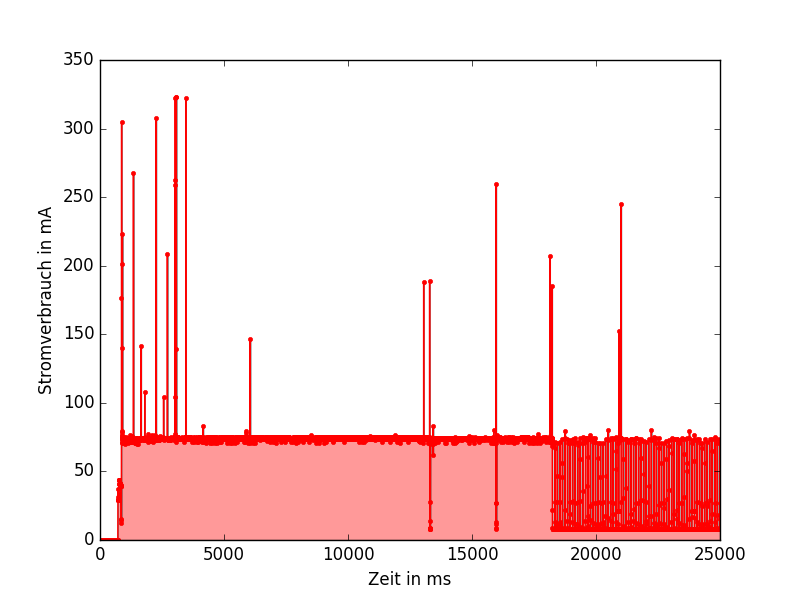
\includegraphics[width=\textwidth]{plots/radar5s.png}
  \caption{Stromverbrauchskurve einer Implementierung von \emph{RADAR}.}
  \label{fig:radar5s}
\end{figure}

Abbildung \ref{fig:radar5ssend} zeigt den Sendevorgang der \emph{RADAR-Implementierung}.
Auffällig ist, dass längerfristig empfangen wird, obwohl dies für den Versand des UDP-Pakets nicht notwendig ist.

\begin{figure}[h!]
  \centering
	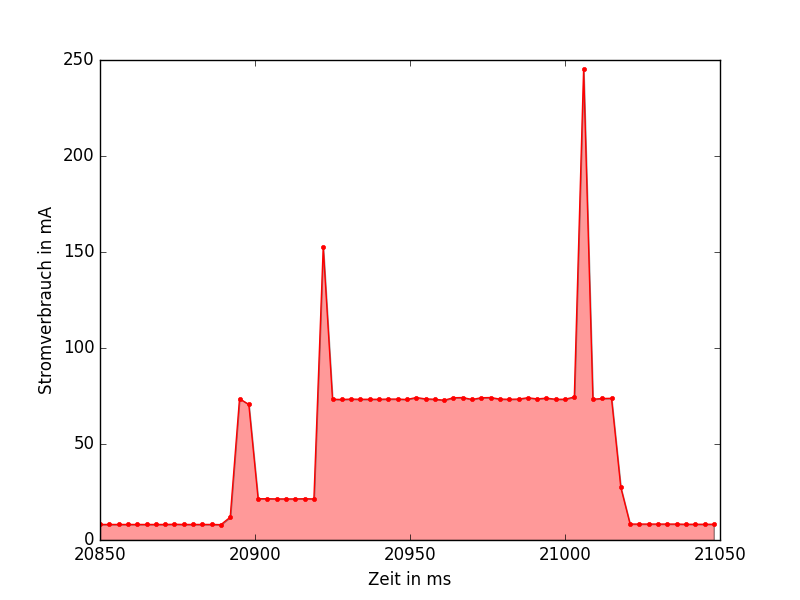
\includegraphics[width=\textwidth]{plots/radar5ssend.png}
  \caption{Stromverbrauchskurve eines Ortungsvorgangs mit RADAR.}
  \label{fig:radar5ssend}
\end{figure}

In Tabelle \ref{table:radarina} ist der durchschnittliche Verbrauch der \emph{RADAR}-Implementierung über eine Stunde gelistet.
Es wurde sowohl mit dem \emph{ESP8266} Feather, als auch mit dem einzelnen \emph{ESP-12F} gemessen, die mobile Einheit wurde jeweils erst circa eine Sekunde nach Beginn mit Strom versorgt.
Für den normalisierten Stromverbrauch wurde der Verbrauch im Ruhezustand subtrahiert. 
Dies beschränkt den Verbrauch auf den für die tatsächliche Funktion nötigen Anteil.

\begin{table}[h!]
	\centering
	\caption{Stromverbrauch mobiler Einheiten mit \emph{RADAR}-Implementierung}
	\label{table:radarina}
	\begin{tabular}{l|l|R{2.5cm}|R{2.5cm}}
		Hardware & Programm & $\varnothing$ Verbrauch in mA (normalisiert) & Laufzeit in Stunden\\
		\hline
		\emph{ESP8266} Feather & RADAR & 16,7 (8,6) & 83,8\\
		\emph{ESP-12F} & RADAR & 10,1 (8,8) & 138,6\\
	\end{tabular}
\end{table}

\subsubsection{Probe-Request-Lokalisierung}
\label{ch:phase2:sec:powerprobereq}
Abbildung \ref{fig:probereqfull} zeigt den Lastverlauf für eine mobile Einheit mit \emph{Probe-Request}-Implementierung und Abbildung \ref{fig:probereqv} zeigt den Lastverlauf für den Sendevorgang. 
Der Verlauf für den \emph{ESP8266} Feather ist in rot und der Verlauf für das \emph{ESP-12F} Moduls ist in grün dargestellt.

Nachdem der \emph{ESP8266} aus dem \texttt{deep\_sleep} erwacht, beginnt eine circa 100 Millisekunden andauerne Startphase, danach sendet er die drei \emph{Probe Requests}.
Anschließend soll der \emph{ESP8266} wieder in den \texttt{deep\_sleep} versetzt werden, vorher empfängt er jedoch noch 100 Millisekunden.
Die restliche Zeit befindet sich der \emph{ESP8266} im Tiefschlaf. 
Bei dem \emph{ESP-12F} Modul ist der INA219 nicht in der Lage einen Stromvebrauch zu messen, er liegt unter 0,1 mA.

\begin{figure}[h!]
  \centering
	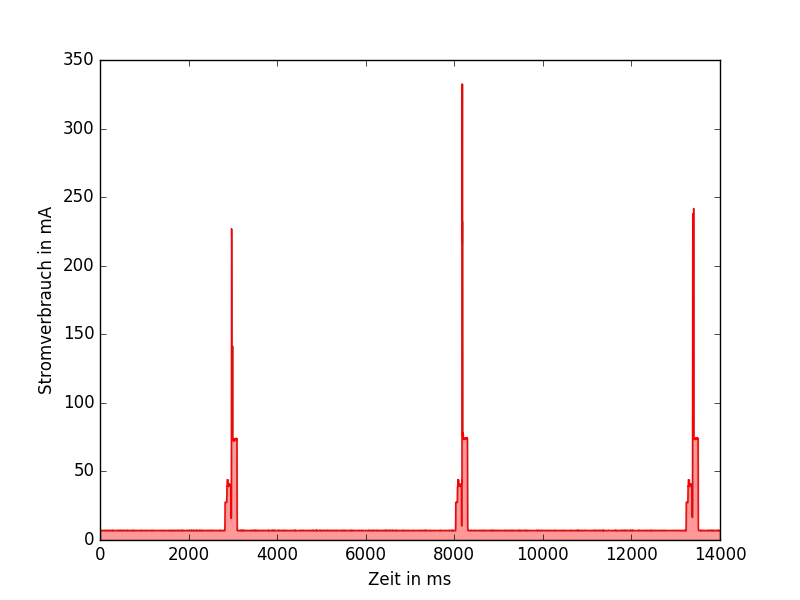
\includegraphics[width=\textwidth]{plots/probereqfull.png}
  \caption{Stromverbrauchskurve einer Implementierung mit \emph{Probe Requests}.}
  \label{fig:probereqfull}
\end{figure}

\begin{figure}[h!]
  \centering
	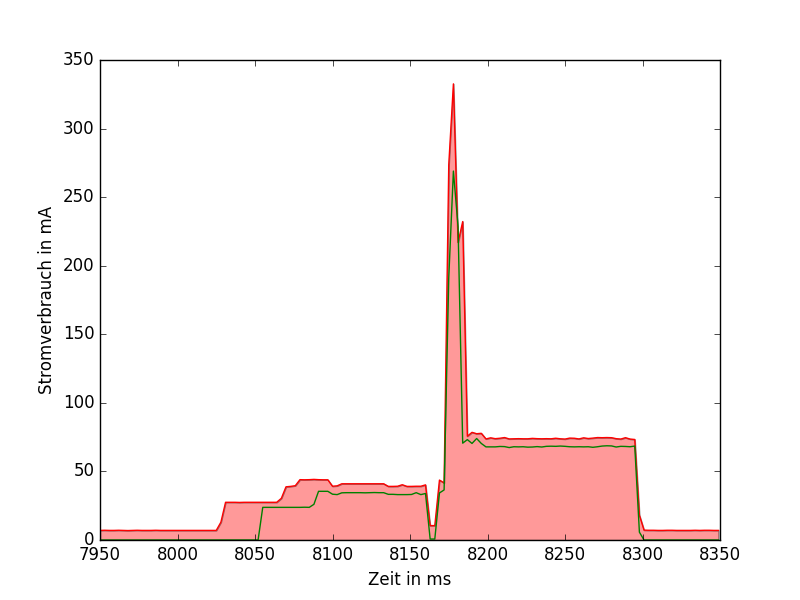
\includegraphics[width=\textwidth]{plots/probereqv.png}
  \caption{Stromverbrauchskurve eines Ortungsvorgangs mit \emph{Probe Requests}.}
  \label{fig:probereqv}
\end{figure}

Beim \emph{ESP8266} Feather misst er jedoch durchgehend einen Vebrauch von über 7 mA, daraus ergeben sich die Unterschiede in den Messungen, die in Tabelle \ref{table:probereqina} dargestellt werden.
Es wurde sowohl mit nur einem versendeten \emph{Probe Request}, als auch mit drei \emph{Probe Requests} getestet, die Unterschiede im Verbrauch liegen jedoch im Bereich der Messungenauigkeit.
Für den normalisierten Stromverbrauch wurde der Verbrauch im Ruhezustand subtrahiert. 
Dies beschränkt den Verbrauch auf den für die tatsächliche Funktion nötigen Anteil.

\begin{table}[h!]
	\centering
	\caption{Stromverbrauch mobiler Einheiten mit \emph{Probe-Request-Lokalisierung}}
	\label{table:probereqina}
	\begin{tabular}{l|p{5.3cm}|R{2.5cm}|R{2.2cm}}
		Hardware & Programm & $\varnothing$ Verbrauch in mA (normalisiert) & Laufzeit in Stunden\\
		\hline
		\emph{ESP8266} Feather & \emph{Probe-Request-Lokalisierung} drei Kanäle & 9,7 (2,7) & 144,0\\
		\emph{ESP-12F} & \emph{Probe-Request-Lokalisierung} drei Kanäle & 1,8 (1,8) & 777,8\\
		\emph{ESP8266} Feather & \emph{Probe-Request-Lokalisierung} ein Kanal & 9,7 (2,7) & 143,7\\
		\emph{ESP-12F} & \emph{Probe-Request-Lokalisierung} ein Kanal & 1,8 (1,8) & 769,2\\
	\end{tabular}
\end{table}

\subsection{Beschleunigungssensor}
\label{ch:Beschleunigungssensor}
Um den Stromverbrauch der \emph{Probe-Request}-basierten Lösung weiter zu senken wird in diesem Abschnitt die Einbindung eines Beschleunigungssensors, in Anlehnung an die kommerzielle Lösung von Ekahau\footnote{\url{https://www.airistaflow.com/}}, diskutiert. 

Im Tunnel Rastatt, in dem auch die Versuche stattfanden, arbeiten die Bauarbeiter in zwei Schichten zu je 12 Stunden. 
Nach 10 Tagen Schicht hat ein Arbeiter 5 Tage frei, jeder Arbeiter arbeitet also genau ein Drittel der Gesamtzeit. 

Die mobile Einheit behält jedoch derzeit seinen Senderythmus bei, angesichts des hohen Stromverbrauchs beim Senden ist dies ineffizient.
Ein Beschleunigungssensor soll bestimmen, wann die mobile Einheit in Bewegung ist. 
Dadurch wird sie nicht mehr senden, wenn sie nicht getragen wird.

\subsubsection{LIS3DH}
Der \emph{LIS3DH} ist ein Drei-Achsen-Beschleunigungssensor von ST Microelectronics \cite{st2015lis}.
Er zeichnet sich durch einen \emph{ultra-low-power} Modus und einen Pin für externe Unterbrechungen (\emph{Interrupt}) aus.
Der Beschleunigungssensor bietet ein \emph{I²C} und ein \emph{SPI Interface}, um ihn zu konfigurieren.
Der \emph{LIS3DH} benötigt bei einer Frequenz von 1 Hz nur 2 \textmu A (0,002 mA).

Leider konnte bei 1 Hz der \emph{Interrupt} durch Laufbewegungen nicht sicher ausgelöst werden, die Frequenz wurde deshalb auf 10 Hz erhöht.
Für eine Frequenz von 10 Hz im \emph{ultra-low-power} Modus listet das Datenblatt einen Verbrauch von 3 \textmu A.
Abbildung \ref{fig:lis3dh} zeigt eine Platine mit integriertem \emph{LIS3DH}.

\begin{figure}[h]
  \centering
	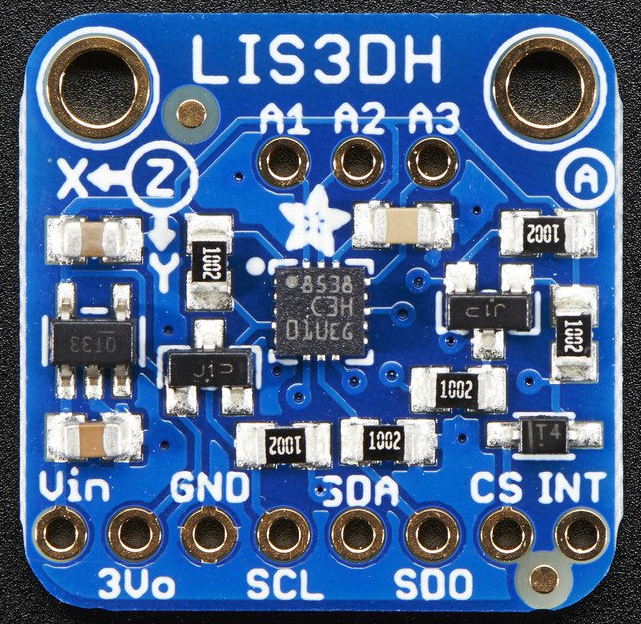
\includegraphics[width=0.5\textwidth]{images/lis3dhada.png}
  \caption{\emph{LIS3DH} integriert auf einer Platine für die Entwicklung. Bild von Adafruit Industries\protect \footnotemark.}
  \label{fig:lis3dh}
\end{figure}
\footnotetext{\url{https://www.adafruit.com/product/2809}}

\subsubsection{Abschaltautomatik}
\label{ch:Beschleunigungssensor:sec:Abschaltautomatik}
Der \emph{ESP8266} besitzt einen \emph{Enable Pin} (CH\_PD), ist dieser mit der Versorungsspannung verbunden, werden die internen Spannungsregler aktiviert und der \emph{ESP8266} mit Strom versorgt.
Die eigentliche Stromversorgung bezieht er dabei jedoch aus dem \emph{Vcc Pin}.
Der \emph{ESP8266} soll durch den \emph{LIS3DH} angeschaltet werden. 
Der \emph{ESP8266} darf die Stromversorgung bei Bedarf trennen, sie kann danach wieder vom \emph{LIS3DH} aktiviert werden. 

Um dieses Verhalten zu erreichen wird ein \emph{Latch} eingesetzt \cite{texas2003latch}.
Es handelt sich dabei um einen digitalen Schalter mit einem SET-Eingang (An), einem RESET-Eingang (Aus) und einem Ausgang.
Der Ausgang wird mit dem \emph{Enable Pin} verbunden, ist er aktiv, wird der \emph{ESP8266} aktiv.
Der SET-Eingang wird mit dem \emph{Interrupt Pin} des \emph{LIS3DH} verbunden, er kann damit den Ausgang aktivieren.
Der RESET-Eingang wird mit dem \emph{ESP8266} verbunden. 
Es wurde \emph{Pin 16} ausgewählt, da dieser für das Aufwecken aus dem Tiefschlaf zuständig ist. 
Stattdessen soll er nun die Stromversorgung abschalten und durch die zuvor im \texttt{deep\_sleep} verbrachte Zeit das Sendeintervall abwarten.

Da das Aufwecken mit \emph{Pin 16} durch das Verbinden des Pins mit der Masse funktioniert, kann damit nicht direkt der RESET-Eingang des Latches betrieben werden.
Stattdessen wird das Ergebnis von \emph{Pin 16} mit der Versorgungsspannung über ein XOR-Gatter verschaltet und mit dem RESET-Eingang verbunden \cite{texas2014xor}.
Abbildung \ref{fig:schematics} zeigt das Schema der Verbindung von \emph{ESP8266} und \emph{LISD3H}.

\begin{figure}[h]
  \centering
	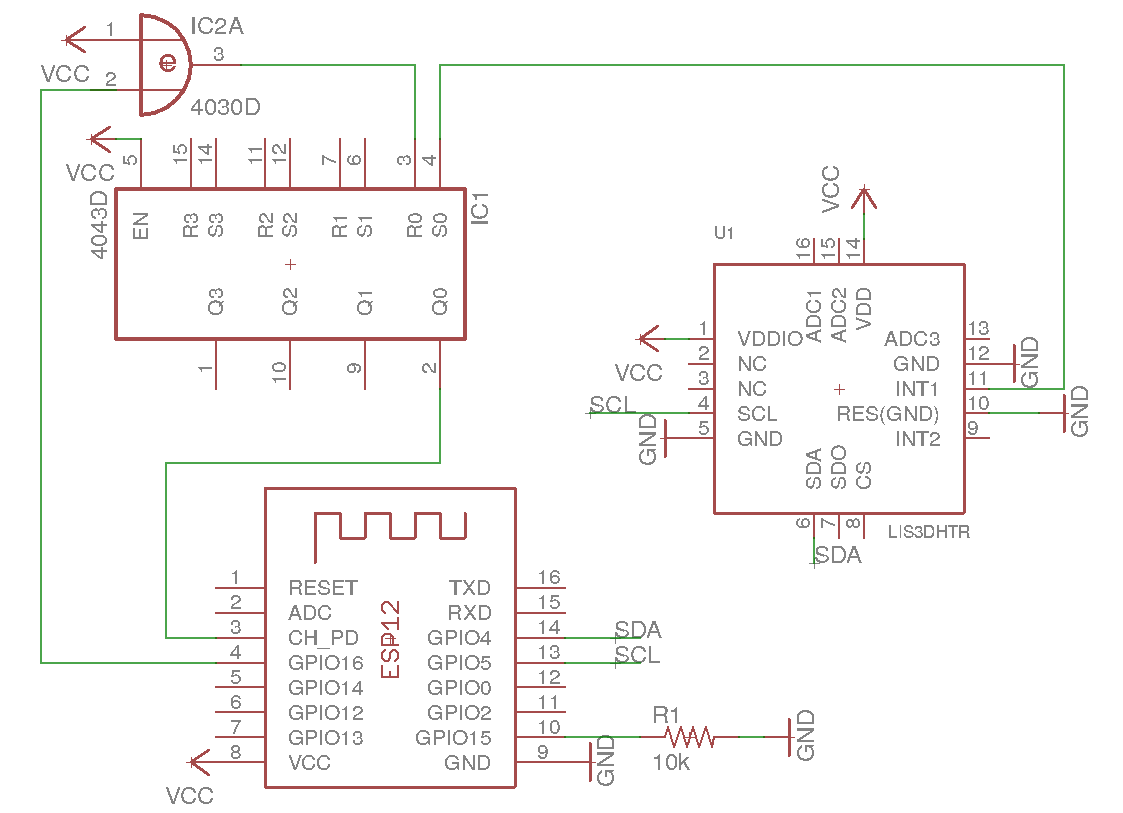
\includegraphics[width=\textwidth]{images/schematics.png}
  \caption{Schema der Verbindung von \emph{ESP8266} und \emph{LIS3DH}.}
  \label{fig:schematics}
\end{figure}

\subsubsection{Bewertung}
Der Verbrauch des Beschleunigungssensors ersetzt lediglich den Verbrauch des Mikrocontrollers, die anderen Komponenten bleiben davon unberührt.
Zu den 3 \textmu A Verbrauch addiert sich deshalb der Verbrauch des Spannungswandlers (55 \textmu A) und des Lithium-Polymer-Ladeschaltkreises (bis zu 100 \textmu A).
Hinzu kommen bis zu 1 \textmu A für das \emph{Latch} und 10 \textmu A für das XOR-Gatter.

Die Integration des Beschleunigungssensor kann also den Verbrauch des \emph{ESP8266} außerhalb der Arbeitszeiten durch einen Verbrauch von 14 \textmu A ersetzen, die bis zu 166 \textmu A Verbrauch der umliegenden Komponenten bleibt jedoch vorhanden.
Die Laufzeit für eine nicht bewegte mobilen Einheit mit \emph{ESP8266} beträgt dann mindestens $1400\ mAh / 0,18\ mA = 7777,77\ h$, dies entspricht ca. 324 Tagen.

Bei den vorherigen Prototypen, die eine \emph{Assoziation} erforderten, muss beachtet werden, dass sie nach dem erneuten Anschalten einen \emph{Scan}- und \emph{Join}-Vorgang ausführen.
Damit diese die Einsparung nicht überwiegen, sollte eine Abschaltung erst nach einigen Minuten der Inaktivität erfolgen.



\section{Direkte Fernlokalisierung mit Bluetooth Low Energy}
\label{ch:phase3}
Für die direkte Fernlokalisierung mit Bluetooth werden dedizierte Basisstationen eingesetzt. 
Die Kommunikation zwischen Basisstation und Ortungsdienst kann durch ein LAN- oder WLAN-Netzwerk gewährleistet werden.
Die Basisstationen bestimmen des \emph{Received Signal Strength Indicator} (RSSI) eingehender Übertragungen der mobilen Enheiten und übermitteln die gemessenen Werte dann an den Ortungsdienst.
Der Ortungsdienst kann mit den gesammelten Werten die Position der mobilen Einheit berechnen.

\subsection{nRF52832}
Der nRF52832 ist eine \emph{System-on-Chip}-Lösung von Nordic Semiconductor.
Er vereint eine 32-bit ARM Cortex-M4F CPU, 512kB RAM und einen 2,4 GHz Transceiver, der Bluetooth 5.0 inklusive Low Energy und das proprietäre ANT Protokoll unterstützt \cite{nordic2017nrf}.

Für diese Arbeit wird ein Adafruit Feather \emph{nRF52} verwendet, der nRF52832 wird deshalb im Folgenden auf \emph{nRF52} abgekürzt.
Das Adafruit Feather \emph{nRF52} besitzt neben dem nRF52832 Spannungswandler für die 3,3 Volt Umwandlung und einen Schaltkreis für die Verwendung mit Lithium Akkus. 
Die verbaute CP2104 USB-to-Serial Schnittstelle erlaubt es, den Chip über USB zu programmieren.

Abbildung \ref{fig:nrf52layout} zeigt das Adafruit Feather nRF52.
Auch Nordic Semiconductor gibt einige typische Stromverbräuche für ihr \emph{System-on-Chip} an, diese sind in Tabelle \ref{table:nrf52consumption} aufgeführt.

\begin{figure}[h]
  \centering
	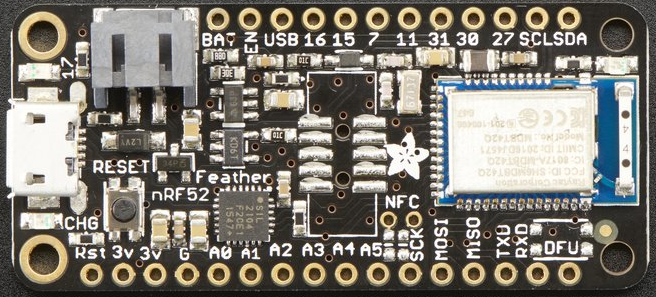
\includegraphics[width=\textwidth]{images/nrf52ada.png}
  \caption{Adafruit \emph{nRF52} Feather. Bild von Adafruit Industries\protect \footnotemark.}
  \label{fig:nrf52layout}
\end{figure}
\footnotetext{\url{https://www.adafruit.com/product/3406}}

\begin{table}[h]
  \centering
  \caption{Stromverbrauch des nRF52832 in verschiedenen Zuständen, aus \cite{nordic2017nrf}}
	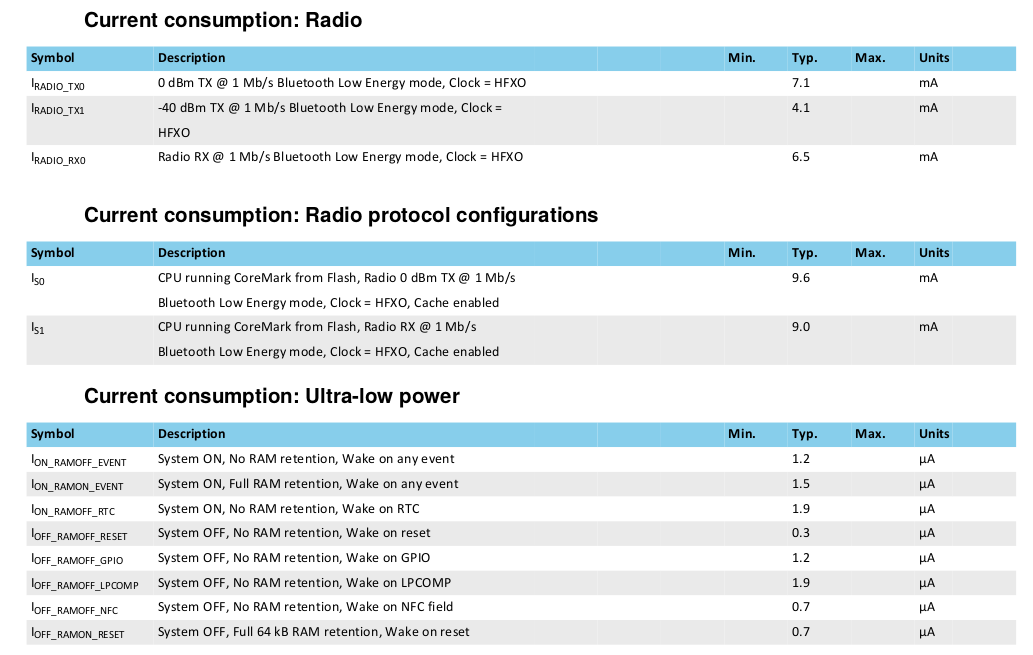
\includegraphics[width=\textwidth]{images/nrf52consumption.png}
  \label{table:nrf52consumption}
\end{table}


\subsubsection{Arduino Bluefruit nRF52 API}
Der \emph{nRF52} kann ebenfalls mit der Arduino IDE programmiert werden.\\
Adafruit stellt eine englischsprachige Anleitung zur Verwendung des \textit{Adafruit Feather nRF52 Bluefruit} mit Arduino zur Verfügung\footnote{\url{https://learn.adafruit.com/bluefruit-nrf52-feather-learning-guide?view=all}}.
Die \emph{Bluefruit nRF52} API stellt dabei Funktionen zur Verwendung von Bluetooth und Bluetooth Low Energy zur Verfügung.
Es wird die \emph{Bluefruit nRF52} API Version 0.6.0 verwendet.



\subsection{Reichweite von Bluetooth Low Energy}
Der Versuch mit BLE wurde an der selben Stelle wie der mit WLAN durchgeführt, siehe dazu Abschitt \ref{ch:phase1:sec:rangewlan}.
Es wurde allerdings ein \emph{Raspberry Pi Zero W} als Basisstation verwendet, dieser wurde auf dem \emph{LN-862} platziert, auf Abbildung \ref{fig:applacement} ist sein rotes Gehäuse zu erkennen.

\subsubsection{Methodik}
Die Reichweite wurde erneut in zwei Richtungen geprüft. 
Zum einen in Richtung der fertig gebohrten Tunnels mit wenigen Hindernissen, zum anderen in Richtung des Vortriebs durch mehrere Stahlhindernisse.
Die zwei Messtrecken werden in Abbildung \ref{fig:rangeblue} skizziert.

\begin{figure}[h!]
  \centering
	\includegraphics[width=\textwidth]{images/rangeblue.eps}
  \caption{Messtrecken zur Festellung der Reichweite von Bluetooth Low Energy.}
  \label{fig:rangeblue}
\end{figure}

Um die Abschirmung durch ein Gehäuse zu simulieren wurde eine stabile Plastikbox verwendet, leider konnte diese nicht vollends geschlossen werden.
Für die Messung wurde der Körper zwischen mobile Einheit und Basisstation gebracht und eine mobile Einheit wurde dann als "`außer Reichweite"' angesehen, wenn versendete Pakete der mobilen Einheit nicht mehr bei der Basisstation ankamen.
Durch das Entfernen des körperlichen Hindernisses war es möglich wieder eine Verbindung herzustellen.

Die bestimmten Reichweiten werden in zwei Meter Schritten angegeben, da sie mit Hilfe der zwei Meter breiten \emph{Tübbinge} bestimmt wurden.

\subsubsection{Ergebnisse}
Tabelle \ref{table:rangeblue} zeigt die Ergebnisse für den nRF52.
Das lose Auflegen des Gehäusedeckels führte zu keiner Veränderung bei der Reichweite.

\begin{table}[h]
	\centering
	\caption{Sendereichweite Bluetooth-basierter mobiler Einheiten}
	\label{table:rangeblue}
	\begin{tabular}{l|l|l|R{3cm}}
		Hardware & Aufbau & Strecke & Maximale Sendereichweite \\
		\hline
		\emph{nRF52} Feather & Offen & Wenige Hindernisse & 32 m \\
		\emph{nRF52} Feather & In Gehäuse & Wenige Hindernisse & 32 m \\
		\emph{nRF52} Feather & Offen & Viele Hindernisse & 14 m \\
		\emph{nRF52} Feather & In Gehäuse & Viele Hindernisse & 14 m \\
	\end{tabular}
\end{table}

\subsubsection{Bewertung}
Um mit 30 km/h 32 Meter zu durchqueren benötigt man 3,8 Sekunden.
Da jedoch eine hohe Erkennungszuverlässigkeit gefordert wurde, sollte das Sendeintervall niedriger gesetzt werden, es wird auf eine Sekunde gesetzt.
Damit werden auch bei einer Reichweite von nur 14 Metern auf der Tunnelbohrmaschine ausreichend viele Pakete versenden um den Verlust einzelner zu kompensieren.

\subsection{BLE-Advertising-Implementierung}
\label{ch:phase3:sec:advertising}
Die \emph{Bluetooth-Low-Energy-Implementierung} ist an die Arbeit von Jianyong et al. angelehnt.
Es wird immer nach Ablauf des Sendeintervalls ein \emph{Advertising} Paket gesendet.

In der Praxis wird dazu das \emph{Advertising}-Intervall entsprechend gesetzt, dabei handelt es sich um einen in Bluetooth 4.0 spezifizierten Parameter für die Häufigkeit des \emph{Advertisings}.
Da die \emph{Bluefruit} \emph{nRF52} API keine Funktion zur Änderung dieses Wertes zur Verfügung stellt muss er direkt geändert werden.
Die entsprechende \emph{BLEAdvertising}-Klasse ist in \\\texttt{/.arduino15/packages/adafruit/hardware/nrf52/0.6.0/libraries/}\\\texttt{Bluefruit52Lib/src} zu finden. 

In \texttt{BLEAdvertising.cpp} ist \texttt{GAP\_ADV\_INTERVAL\_MS} auf 20 Millisekunden gesetzt, dieser Wert sollte erhöht werden, um den Stromverbrauch zu senken.
Beim \emph{nRF52} handelt es sich um ein Klasse 2 Bluetooth-Gerät mit einer maximalen Sendeleistung bis 4 dBm.
Das Sendeintervall wird etsprechend der Untersuchung der Reichweite und maximalen Bewegungsgeschwindigkeit von 30 km/h auf eine Sekunde gesetzt, in dieser Zeit kann sich ein Mitarbeiter maximal 9 Meter bewegen.

Es sollte erneut eine Voruntersuchung des Verbrauchs mit dem Muker \emph{TM103} USB-Power-Meter vorgenommen werden.
Diser ist aber nicht in der Lage den Stromverbrauch des \emph{nRF52} zu messen.
Die Sendeabschnitte sind zu kurz um einen messbaren Stromverbrauch zu erzeugen.

Deshalb wird zunächst Abbildung \ref{table:nrf52consumption} für eine theoretische Betrachtung des Verbrauchs herangezogen werden. 




\subsection{Untersuchung des Stromverbrauchs}
Der Stromverbrauch soll mit dem INA219 genauer bestimmt werden, der INA219 und die verwendete Methodik werden in Abschnitt \ref{ch:phase1:sec:energie} beschrieben.

\subsubsection{Theoretische Stromverbrauchsabschätzung}
Für die Zeit in der nicht gesendet wird, wird der Zustand $I_{ON\_RAMOFF\_RTC}$ angenommen, da dieser den höchsten Verbrauch aufweist.
Für die Sendezeit wird $I_{RADIO\_TX0}$ angenommen, für ein \emph{Advertising}-Paket, welches zusätzlich den Gerätenamen "`TestTag"' versendet, werden 24 Bytes (192 Bit) gesendet.
Um die Kollisionsvermeidung einzufügen werden vorher 2000 Bit im Zustand $I_{RADIO\_RX0}$ empfangen, der die restliche Zeit wird in $I_{ON\_RAMOFF\_RTC}$ verbracht. 
Es müssen ebenfalls die weiteren Komponenten auf dem Feather bedacht werden. 
Adafruit gibt für den Spannungswandler einen Verbrauch von 55 \textmu A und für den Lithium-Polymer-Ladeschaltkreis einen Verbrauch von bis zu 100 \textmu A an \cite{fried2016lora}. 
Der Verbrauch des anderen Komponenten des Feather wird daher konservativ auf 155 \textmu A geschätzt.
Damit ergibt sich ein durchschnittlicher Verbrauch $y$ in Höhe von: 

$y = (1s-\frac{Bits\_gesendet}{1000000 b/s} - \frac{Bits\_empfangen}{1000000 b/s}) * (I_{ON\_RAMOFF\_RTC} + 155 {\mu}A) + \frac{Bits\_gesendet}{1000000 b/s} * I_{RADIO\_RX0} + \frac{Bits\_empfangen}{1000000 b/s} * I_{RADIO\_RX0}$

$y = (1s - 0,000192s - 0,002s) * 0,1569mA + 0,000192 * 7,1mA + 0,002 * 6,5mA$

$y \approx 0,156556mA + 0,001363mA + 0,013mA = 0,170919mA$ 

\subsubsection{Tatsächlicher Stromverbrauch von BLE}
\label{ch:phase3:sec:powerble}
Abbildung \ref{fig:blue} zeigt den Lastverlauf für den Start einer mobilen Einheit mit Bluetooth-Low-Energy-Advertising.

Zu Beginn ist eine Startphase zu erkennen, ab 2 Sekunden nach Start des Experiments ist dann das regelmäßige Muster aus Verbrauch im Ruhezustand und kurzen Verbrauchsspitzen beim Senden zu erkennen.
Die Kürze des Sendevorgangs bedingt die starke Schwankung bei den Lastspitzen, die Samplingrate von 333 Hz reicht hier offenbar nicht aus um dem Sendevorgang vollständig zu erfassen.

\begin{figure}[h!]
  \centering
	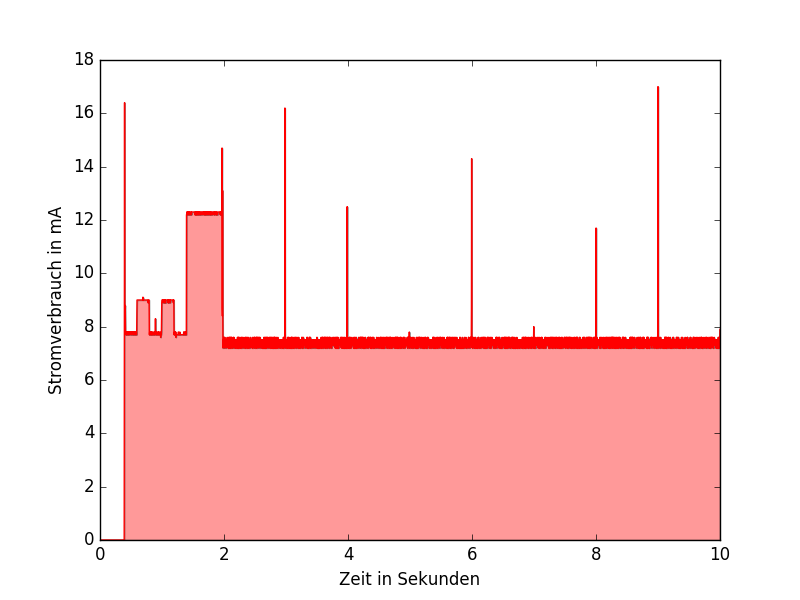
\includegraphics[width=\textwidth]{plots/blue.png}
  \caption{Stromverbrauchskurve einer Implementierung von Bluetooth-Low-Energy-Advertising.}
  \label{fig:blue}
\end{figure}

Hauptverbrauch liegt jedoch in den 7,2 bis 7,6 mA im Ruhezustand, leider ist in diesem Fall kein einzelnes Modul vorhanden, es kann nur auf dem \emph{nRF52} Feather gemessen werden.
Tabelle \ref{table:blueina} zeigt deshalb neben dem gemessenen Verbrauch den normalisierten Stromverbrauch, dafür wurde der Verbrauch im Ruhezustand subtrahiert. 
Dies beschränkt den Verbrauch auf den für die tatsächliche Funktion nötigen Anteil.

\begin{table}[h!]
	\centering
	\caption{Stromverbrauch mobiler Einheiten mit Bluetooth-Low-Energy-Advertising}
	\label{table:blueina}
	\begin{tabular}{p{3.5cm}|p{5cm}|R{2.5cm}|R{2.5cm}}
		Hardware & Programm & $\varnothing$ Verbrauch in mA (normalisiert) & Laufzeit in Stunden\\
		\hline
		\emph{nRF52} Feather & Bluetooth-Low-Energy-Advertising & 7,37 (0,04) & 190\\
	\end{tabular}
\end{table}


\section{Direkte Fernlokalisierung mit Long Range}
\label{ch:phase4}
Für die direkte Fernlokalisierung mit \emph{Long Range} (LoRa) werden dedizierte Basisstationen eingesetzt. 
Die Kommunikation zwischen Basisstation und Ortungsdienst kann durch ein LAN- oder WLAN-Netzwerk gewährleistet werden.
Die Basisstationen bestimmen den \emph{Received Signal Strength Indicator} (RSSI) eingehender Übertragungen der mobilen Enheiten und übermitteln die gemessenen Werte dann an den Ortungsdienst.
Der Ortungsdienst kann mit den gesammelten Werten die Position der mobilen Einheit berechnen.

\subsection{RFM95}
\label{ch:hardwarechanges:sec:rfm95}
Bei dem \emph{RFM95} handelt es sich um ein LoRa-fähiges Radio-Modul für den Frequenzbereich 868/915 MHz \cite{hope2006rfm}. 
915 MHz sind jedoch nur in Amerika lizenzfrei, in Deutschland muss das Radio mit 868 MHz betrieben werden.

Für die Entwicklung wird das Modul auf einem Adafruit Feather M0 \emph{RFM95} LoRa Radio verwendet.
Dieses verwendet einen M0 Mikrocontroller zur Steuerung, einen Lithium-Akku-Ladeschaltkreis und einen Spannungswandler.
Zusätzlich ist eine Antenne notwendig. 
Die verwendete Antenne kann dabei einen große Unterschiede in der Reichweite verursachen, deshalb sollte eine Antenne für 868 MHz verwendet werden.
Da jedoch eine feste Antenne die mobile Einheit unhandlich machen würde, wird für diese eine Kabelantenne verwendet, diese hat die Länge einer halben Wellenlänge (17,3 cm).

Abbildung \ref{fig:lorafeather} zeigt ein Adafruit Feather M0 \emph{RFM95} LoRa Radio. 
Für die Basisstation wird ein Feather M0 \emph{RFM95} LoRa Radio mit fester Antenne verwendet.

\begin{figure}[h]
  \centering
	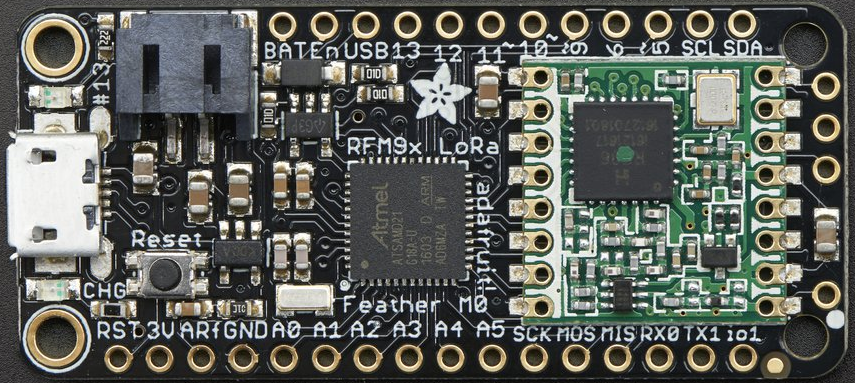
\includegraphics[width=\textwidth]{images/loraada.png}
  \caption{Adafruit Feather M0 \emph{RFM95} LoRa Radio. Bild von Adafruit Industries\protect \footnotemark.}
  \label{fig:lorafeather}
\end{figure}
\footnotetext{\url{https://www.adafruit.com/product/3178}}

\subsubsection{RadioHead RFM9x für Arduino}
Der M0 Mikrocontroller ist Arduino kompatibel, wird zusätzlich die \emph{RadioHead RFM9x} Bibliothek verwendet, kann er über ein \emph{SPI Interface} das Radio steuern.
Adafruit stellt dazu eine englischsprachige Anleitung zur Verfügung\footnote{\url{https://learn.adafruit.com/adafruit-feather-m0-radio-with-lora-radio-module/setup}}.
Es wird die \emph{RadioHead RFM9x} Bibliothek Version 1.62 verwendet.

\subsection{Reichweite von LoRa}
Die Versuche mit LoRa wurden an einer anderen Tunnelbaustelle durchgeführt.
An der Tunnelbaustelle Ulm wird mit Sprengungen vorgetrieben.
Nach der Sprengung wird der Tunnel mit Spritzbeton ausgekleidet und danach wird in drei Schritten geschalt. 
Im ersten Schritt wird ein Filz und eine Folie gegen das Eindringen von Wasser eingebracht, danach folgt die Bewehrung und abschließend wird die Bewehrung einbetoniert.
Für jeden Schritt wird ein stählerner Schalungswagen verwendet, folglich sind drei stählerne Hindernisse im Tunnel, die Signale absorbieren.
Abbildung \ref{fig:schalungswagen} zeigt einen der Schalungswagen, der als Hindernis gedient hat.

\begin{figure}[h]
  \centering
	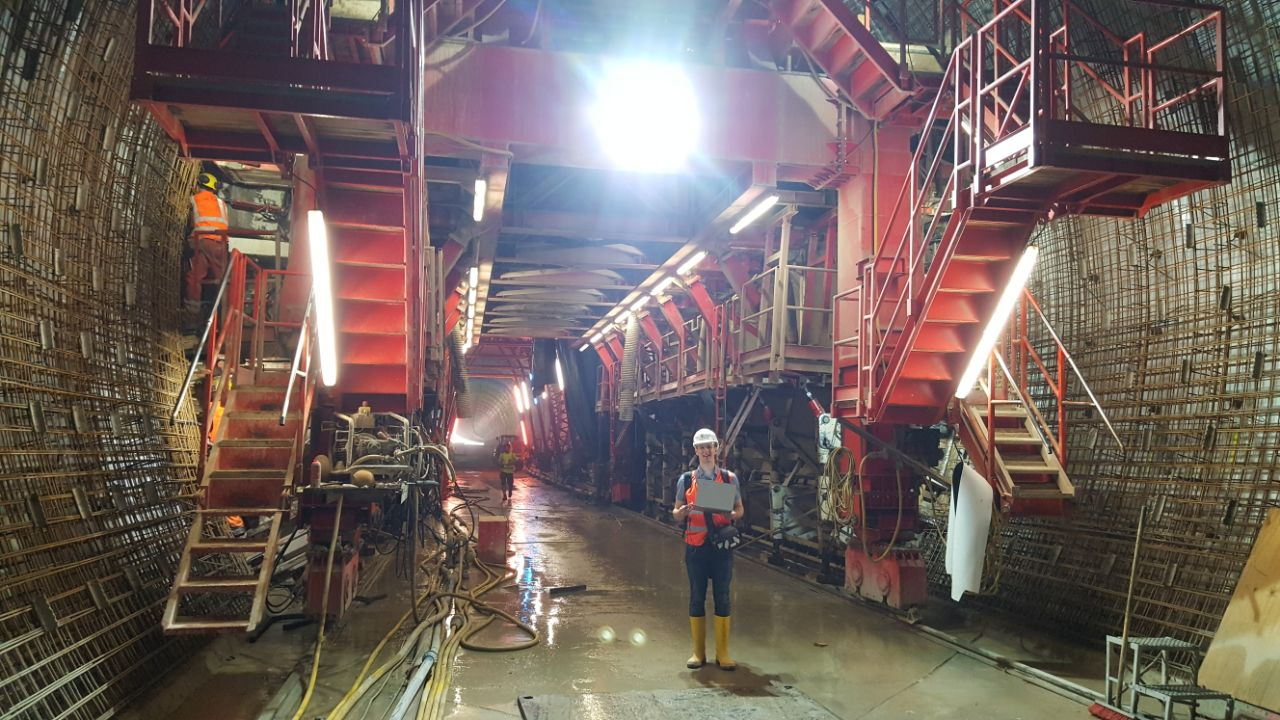
\includegraphics[width=\textwidth]{images/schalungswagen.jpg}
  \caption{Schalungswagen für das Betonieren im Tunnel Ulm.}
  \label{fig:schalungswagen}
\end{figure}

\subsubsection{Methodik} 
Die Reichweite wurde für zwei Situationen bestimmt.
Zum einen durch einen Schalungswagen und dann durch den freien Tunnel, zum anderen durch alle drei Schalungswagen für eine Situation mit maximaler Abschirmung durch die Hindernisse.
Die zwei Messtrecken werden in Abbildung \ref{fig:rangelora} skizziert.

\begin{figure}[h!]
  \centering
	\includegraphics[width=\textwidth]{images/rangelora.eps}
  \caption{Messtrecken zur Festellung der Reichweite von LoRa.}
  \label{fig:rangelora}
\end{figure}

Die mobile Einheit wurde jeweils direkt an der Bewehrung platziert und es wurde auf der selben Seite gelaufen, damit die Abschirmung durch die Schalungswagen maximal ist.
Danach wurde die Basisstation immer weiter entfernt, bis keine Pakete der mobilen Einheit mehr empfangen werden konnten.
Abbildung \ref{fig:lorabasis} zeigt die Platzierung der mobilen Einheit an der Bewehrung.
Erneut konnte die Plastikbox aufgrund des Versuchsaufbaus nicht geschlossen werden.

Die mobile Einheit wurde als "`außer Reichweite"' angesehen, wenn versendete Pakete der mobilen Einheit nicht mehr bei der Basisstation ankamen.
Durch das Entfernen des körperlichen Hindernisses war es möglich wieder eine Verbindung herzustellen.
Es wurde sowohl mit einer Sendeleistung von 5 dBm für einen geringen Sendeverbrauch als auch mit 23 dBm Sendeleistung für maximale Reichweite gemessen.
Die Messungen werden in 12,5 m Abständen angegeben, da in diesem Tunnel die Länge eines Schalungselements 12,5 m beträgt.
Es werden, wie in Abschnitt \ref{ch:hardwarechanges:sec:rfm95} besprochen, zwei unterscheidliche Typen von Antennen verwendet. 
Während die Basisstation eine feste Antenne aufweist, verwendet die mobile Einheit eine Kabelantenne entsprechend der halben Wellenlänge. 

\begin{figure}[h]
  \centering
	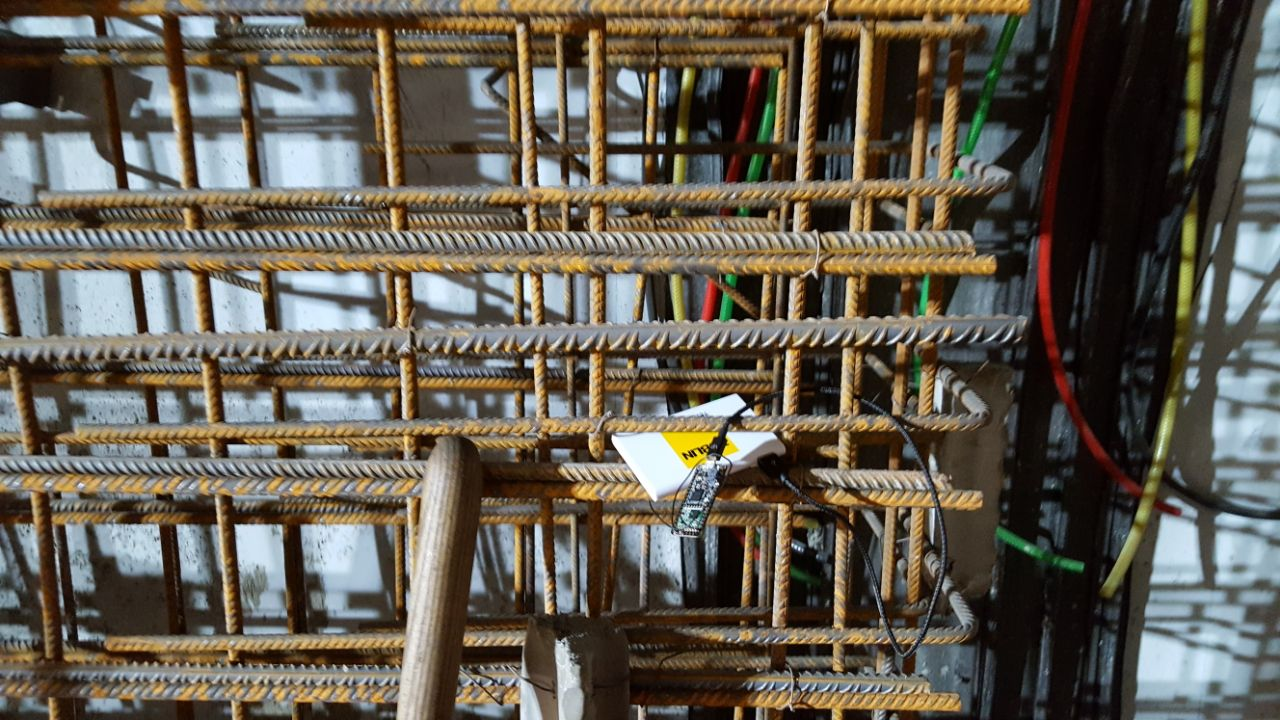
\includegraphics[width=\textwidth]{images/lorabasis.jpg}
  \caption{Platzierung der mobilen Einheit an der Bewehrung des Tunnels.}
  \label{fig:lorabasis}
\end{figure}

\subsubsection{Ergebnisse}
Tabelle \ref{table:rangelora} zeigt die Ergebnisse für das \emph{RFM95}.
Da das lose Auflegen des Deckels der Plastikbox zu keiner Veränderung bei der Reichweite führte gibt die Tabelle nur Werte für den offenen Aufbau an. 
Der Test mit 23 dBm Sendeleistung durch alle drei Schalungswagen musste nach 350 m abgebrochen werden, weil ein weiterkommen nicht möglich war.
Da jedoch für diese Sendeleistung bereits nach circa 250 m die Varianz des RSSI den Zusammenhang zwischen Distanz und RSSI überwiegt, kann die tatsächliche Reichweite dieser Sendeleistung nicht ausgenutzt werden.
Für eine sichere Erkennung des 250-Meter-Abschnitts müsste daher alle 500 m eine Basisstation aufgestellt werden.

\begin{table}[h]
	\centering
	\caption{Sendereichweite LoRa-basierter mobiler Einheiten}
	\label{table:rangelora}
	\begin{tabular}{p{2.2cm}|p{1.5cm}|R{2.5cm}|p{3.5cm}|R{3cm}}
		Verwendetes Modul & Aufbau & Sendeleistung & Strecke & Maximale Sendereichweite \\
		\hline
		\emph{RFM95} & Offen & 5 dBm & Wenige Hindernisse & 250 m \\
		\emph{RFM95} & Offen & 5 dBm & Viele Hindernisse & 100 m \\
		\hline
		\emph{RFM95} & Offen & 23 dBm & Wenige Hindernisse & 1250 m \\
		\emph{RFM95} & Offen & 23 dBm & Viele Hindernisse & >350 m \\
	\end{tabular}
\end{table}

\subsubsection{Bewertung}
LoRa entfaltet im Tunnel eine sehr hohe Reichweite und es kann eine lückenlose Überwachung von Personen durchgeführt werden.
Voll nutzen lässt sich die Reichweite jedoch nicht, da die Varianz des RSSI den Zusammenhang zwischen Distanz und RSSI schon nach circa 250 m überwiegt. 
Hingegen führt eine starke Reduktion der Sendeleistung zu einer mangelnder Penetration von Hindernissen.
Daher sollte ein Kompromiss der Sendeleistung geschlossen werden. 
Eine Sendeleistung von 10 dBm sollte eine ausreichende Reichweite im Szenario mit vielen Hindernissen bieten.
Alternativ kann die mobile Einheit auch ein \emph{Send-Receive-Schema} umsetzen und von der Basisstation eine dynamisch angepasste Sendeleistung empfangen, die sich nach der Menge der Hindernisse richtet.

Wird die Sendeleistung dynamisch so festgelegt, dass eine Reichweite von 250 Metern erreicht wird, benötigt ein Mitarbeiter bei 30 km/h 30 Sekunden, um sie zu durchqueren.
Eine derart lange Intervallzeit würde jedoch dazu führen, dass eine volle Minute ohne Aktualisierung der Position vergeht, sollte ein Paket verloren gehen.
Das Sendeintervall wird deshalb auf 10 Sekunden gesetzt.

\subsection{LoRa-Implementierung}
Die Implementierung für die Lokalisierung mit LoRa ist sehr simpel.
Die mobile Einheit versendet regelmäßig ein Paket, welches einen Identifikator für die mobile Einheit enthält.
Das Sendeintervall beträgt entsprechend der hohen Reichweite 10 Sekunden.

Die Basisstation empfängt durchgehend und bestimmt den RSSI für eingehende Pakete.
Anschließend leitet sie den Identifikator der mobilen Einheit zusammen mit dem RSSI und einer Kennung für die Basisstation an den Ortungsdienst weiter.

Auf der mobilen Einheit müssen lediglich die Sendefrequenz, die Sendeleistung und der Identifikator gesetzt werden, dann kann immer nach Ablauf des Sendeintervalls gesendet werden.
Die Basisstation muss dabei auf der selben Frequenz aktiv sein und empfangen.


\subsection{Untersuchung des Stromverbrauchs}
Der Stromverbrauch soll mit dem INA219 genauer bestimmt werden, der INA219 und die verwendete Methodik werden in Abschnitt \ref{ch:phase1:sec:energie} beschrieben.

\subsubsection{Theoretische Stromverbrauchsabschätzung}
Für die Berechnung des theroretischen Verbrauchs der mobilen Einheit werden die Datenblätter des M0 Mikrocontrollers und des \emph{RFM95} Radios herangezogen. 
Die dort gelisteten Verbräuche sind in Tabelle \ref{table:m0power} und Tabelle \ref{table:lorapower} zu finden.

\begin{table}[h]
  \centering
  \caption{Stromverbrauch des M0 Mikrocontrollers, aus \cite{nxp2016m0}}
	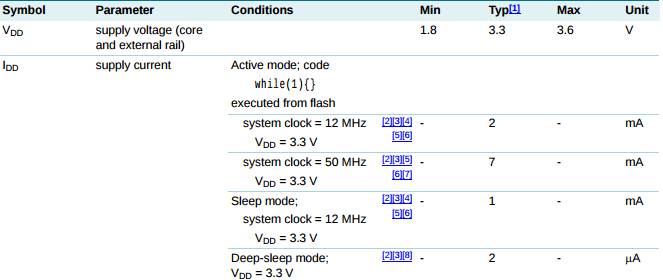
\includegraphics[width=\textwidth]{images/m0power.png}
  \label{table:m0power}
\end{table}

\begin{table}[h]
  \centering
  \caption{Stromverbrauch des \emph{RFM95}, aus \cite{hope2006rfm}}
	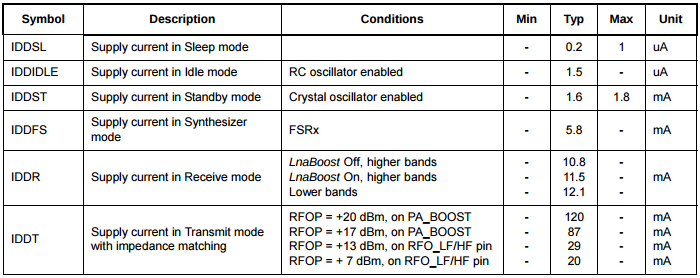
\includegraphics[width=\textwidth]{images/lorapower.png}
  \label{table:lorapower}
\end{table}

Da das Adadfruit Feather M0 \emph{RFM95} Lora Radio sich nur durch die Ersetzung des \emph{CP2014} durch den \emph{Cortex-M0} zum Adafruit Feather \emph{nRF52} unterscheidet werden die 155 \textmu A für die sonstigen Komponenten übernommen.

Die Sendeleistung des \emph{RFM95} Radio ist zwischen 5 dBm und 23 dBm einstellbar. 
Das Datenblatt listet jedoch nur Verbräuche zwischen 7 dBm und 20 dBm Sendeleistung, der Verbrauch wird für diese beiden Sendeleistungen berechnet.
Für die Nachricht "`TagTest"' werden 20 Bytes (160 Bits) versendet, es wird angenommen, dass zuvor 500 Bits für die Kollisionskontrolle belauscht werden.
Für die restliche Zeit wird angenommen, dass sich der \emph{M0} Mikrocontroller im \emph{Deep-sleep mode} und das \emph{RFM95} Radio im \emph{IDDIDLE} Modus befindet.
Damit ergibt sich ein durchschnittlicher Verbrauch $y$ in Höhe von: 

$y = \frac{1}{10} * [(10 - \frac{Bits\_gesendet}{21875 b/s} - \frac{Bits\_empfangen}{21875 b/s}) * (M0\_Deep\_sleep\_mode + RMF95\_IDDIDLE + 155 {\mu}A) + \frac{Bits\_gesendet}{21875 b/s} * RFM95\_XdBm + \frac{Bits\_empfangen}{21875 b/s} * RFM95\_IDDR]$

Für die folgende Rechnung wird eine Sendeleistung von 20 dBm angenommen:

$y_{20dBm} = \frac{1}{10} * [(10s - 0,0073s - 0,0229s) * 0,1585mA + 0,0073s * 120mA + 0,0229s * 12,1mA]$\\[0.5cm]
$y_{20dBm} \approx \frac{1}{10} * (1,58mA + 0,876mA + 0,2771mA) = 0,2683mA$

Als Stromsparmaßnahme wird für die folgende Rechnung die Sendeleistung auf 7 dBm reduziert:

$y_{7dBm} = \frac{1}{10} * [(10s - 0,0073s - 0,0229s) * 0,1585mA + 0,0073s * 20mA + 0,0229s * 12,1mA]$\\[0.5cm]
$y_{7dBm} \approx \frac{1}{10} * (1,58mA + 0,146mA + 0,2771mA) = 0,1953mA$

\subsubsection{Tatsächlicher Stromverbrauch von LoRa}
\label{ch:phase3:sec:powerlora}
Der Stromverbrauch der Implementierung mit LoRa wurde mit 5 dBm und 23 dBm Sendeleistung überprüft.
Abbildung \ref{fig:lora5} zeigt den Lastverlauf für den Start einer mobilen Einheit mit LoRa bei 5 dBm.

Nach einer circa 3-sekündigen Startphase wechselt der LoRa Feather in den regulären Betrieb, er sollte dann immer nach 10 Sekunden Ruhezustand senden.
Dieser jedoch vom Zeitgeber nicht ganz eingehalten, die mobile Einheit befindet sich zwischen den Sendevorgängen circa 11 Sekunden im Ruhezustand, dies sollte bei der Implementierung beachtet werden.
Im Ruhezustand liegt der Verbrauch des LoRa Feather bei 0,9 bis 1,0 mA, beim Senden unterscheiden sich die Vebräuche je nach Sendeleistung deutlich.

\begin{figure}[h!]
  \centering
	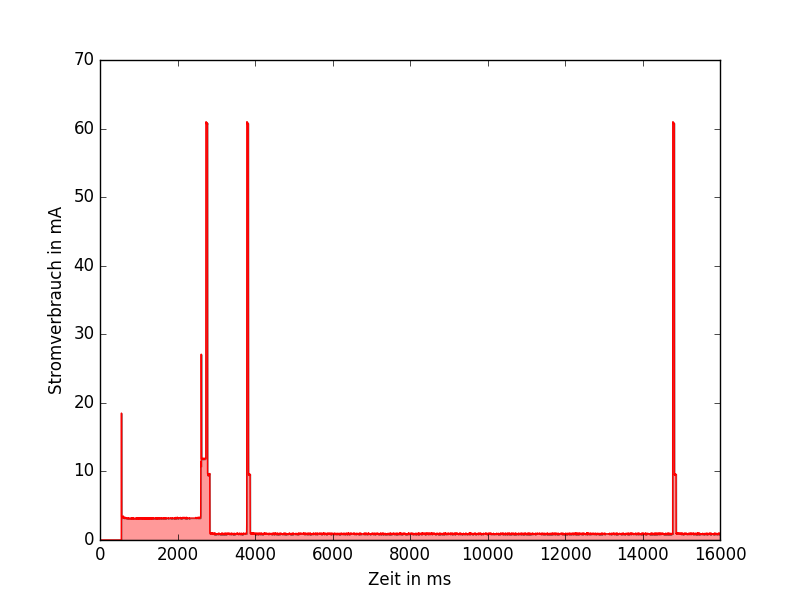
\includegraphics[width=\textwidth]{plots/lora5.png}
  \caption{Stromverbrauchskurve einer Implementierung mit LoRa.}
  \label{fig:lora5}
\end{figure}

Die Abbildung \ref{fig:lora235send} zeigt die Sendeverbräuche für eine Sendeleistung von 23 dBm in Rot und für 5 dBm in Grün.
Gut zu erkennen ist hier auch, dass ein Sendevorgang bei LoRa deutlich länger als bei BLE dauert, obwohl vergleichbar viele Bits übertragen werden.

\begin{figure}[h!]
  \centering
	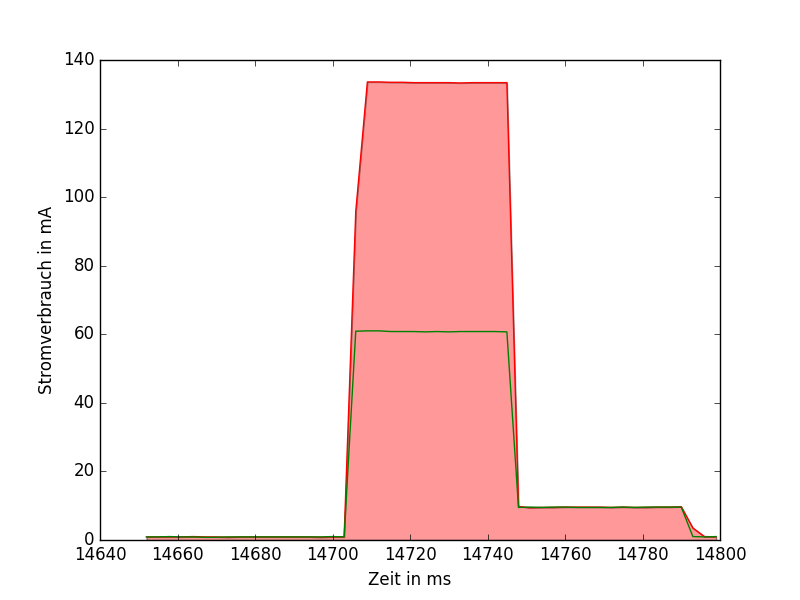
\includegraphics[width=\textwidth]{plots/lora235send.png}
  \caption{Stromverbrauchskurve eines Ortungsvorgangs mit LoRa.}
  \label{fig:lora235send}
\end{figure}

Die Ergebnisse der Messungen sind in Tabelle \ref{table:lora235ina} gelistet.
Für den \emph{RFM95} Feather liegt der Ruheverbrauch deutlich niedriger, da jedoch die selben Schaltungen für Akku-Ladung und Spannungsregelung zum Einsatz kommen, scheint der \emph{CP2104}, welcher zum Programmieren des \emph{ESP8266} beziehungsweise \emph{nRF52} dient, mindestens 6 mA zu verbrauchen.
Für den normalisierten Stromverbrauch wurde der Verbrauch im Ruhezustand subtrahiert. 
Dies beschränkt den Verbrauch auf den für die tatsächliche Funktion nötigen Anteil.

\begin{table}[h!]
	\centering
	\caption{Stromverbrauch mobiler Einheiten mit LoRa}
	\label{table:lora235ina}
	\begin{tabular}{l|l|R{2.5cm}|R{2cm}}
		Hardware & Programm & $\varnothing$ Verbrauch in mA (normalisiert) & Laufzeit in Stunden\\
		\hline
		LoRa Feather & LoRa 23 dBm Sendeleistung & 1,47 (0,57) & 952,4\\
		LoRa Feather & LoRa 5 dBm Sendeleistung & 1,20 (0,30) & 1166,7\\
	\end{tabular}
\end{table}






\section{Zusammenfassung}
Die folgenden Abschnitte sollen die Ergebnisse des Kapitels zusammenfassen und aufarbeiten.

\subsection{Reichweite}
Die Zuverlässigkeit bei der Erkennung von Bereichswechseln hängt maßgeblich von der Reichweite der Funktechnologie und der Länge des Sendeintervalls ab.
Tabelle \ref{table:ranges} fasst die Ergebnisse der Versuche zur Reichweite zusammen. 
Es wurden jeweils Ergebnisse ohne Gehäuse ausgewählt, da die Reichweite durch ein Gehäuse nur im Falle des \emph{ESP-12S} zu einer Verringerung der Reichweite geführt hat. 
Die Ergebnisse des \emph{ESP-12S} sind jedoch zugunsten des \emph{ESP-12F} nicht gelistet.

\begin{table}[h]
	\centering
	\caption{Sendereichweite mobiler Einheiten}
	\label{table:ranges}
	\begin{tabular}{l|l|l|R{3cm}}
		Protokoll & Verwendetes Modul & Strecke & Maximale Sendereichweite \\
		\hline
		IEEE 802.11b & \emph{ESP-12F} & Wenige Hindernisse & 88 m \\
		BLE 5.0 & \emph{nRF52} & Wenige Hindernisse & 32 m \\
		LoRa & \emph{RFM95} 5 dBm & Wenige Hindernisse & 250 m \\
		LoRa & \emph{RFM95} 23 dBm & Wenige Hindernisse & 1250 m \\
		\hline
		IEEE 802.11b & \emph{ESP-12F}  & Viele Hindernisse & 32 m \\
		BLE 5.0 & \emph{nRF52}  & Viele Hindernisse & 14 m \\
		LoRa & \emph{RFM95} 5 dBm & Viele Hindernisse & 100 m \\
		LoRa & \emph{RFM95} 23 dBm & Viele Hindernisse & >350 m \\
	\end{tabular}
\end{table}

Der Abstand der Basisstationen für die Bereichsortung ist mit 250 Metern gegeben. 
Die einzige Funktechnologie, die über 125 Meter im Tunnel erreichte, ist LoRa.
Sie ist deshalb die einzige getestete Funktechnologie, die eine lückenlose Ortung ermöglicht.
Zu beachten ist, dass LoRa keine Kollisionsvermeidung verwendet, stattdessen wird auf einem zufälligem Kanal gesendet.
Es muss davon ausgegangen werden, dass manche Nachrichten verloren gehen.
Das Sendeintervall sollte deshalb deshalb nur auf die Hälfte des gewünschten Ortungsintervalls gesetzt werden. 
Um das Problem durch redundantes Senden zu umgehen, wurde das Sendeintervall in dieser Arbeit auf 10 Sekunden gesetzt.

Bei BLE und IEEE 802.11 entscheidet die Reichweite über das Sendeintervall, da hier Versorungslücken bei der jeweiligen Funktechnologie entstehen.
Sie werden dabei so gesetzt, dass beim Durchqueren des abgedeckten Bereichs mit 30 km/h mehrfach gesendet wird.
In dieser Arbeit wurden die Sendeintervalle für IEEE 802.11 auf 5 Sekunden und für BLE auf eine Sekunde gesetzt.

Kürzere Sendeintervalle führen dabei zu einer höheren Erkennungszuverlässigkeit, längere Sendeintervalle senken den Stromverbrauch.

\subsection{Mobile Einheiten}
Im Laufe dieser Arbeit wurden mehrere mobile Einheiten implementiert, diese sind in Tabelle \ref{table:implemen} gelistet.

\begin{table}[h]
	\centering
	\caption{Implementierungen}
	\label{table:implemen}
	\begin{tabular}{l|l|p{2.5cm}|p{5.8cm}}
		Protokoll & Hardware & Art der Fernlokalisierung & Programm \\
		\hline
		IEEE 802.11 & \emph{ESP8266} & Indirekt & \emph{WiFi-LLS} \cite{chen2007design} \\
		IEEE 802.11 & \emph{ESP8266} & Indirekt & \emph{Assoziations-Lokalisierung} \\
		\hline
		IEEE 802.11 & \emph{ESP8266} & Direkt & \emph{RADAR} \cite{bahl2000radar} \\
		IEEE 802.11 & \emph{ESP8266} & Direkt & \emph{Probe-Request-Lokalisierung} \\
		\hline
		BLE & \emph{nRF52} & Direkt & Ortung mit \emph{Bluetooth-Low-Energy-Advertising} \cite{jianyong2014rssi} \\
		\hline
		LoRA & \emph{RFM95} & Direkt & Ortung mit LoRa RSSI \\
	\end{tabular}
\end{table}

Die Implementierungen \emph{Assoziations-Lokalisierung} und \emph{Probe-Request-Lokalisierung} sind dabei Verbesserungen gegenüber den in der Literatur vorgeschlagenen Implementierungen, um den Stromverbrauch der jeweiligen mobilen Einheit zu senken.
Bei \emph{Ortung mit LoRa RSSI} wurde entgegen der Literatur der RSSI als Messwert gewählt.
Die Konzepte der anderen Implementierungen entspringen der Literatur.

\subsection{Stromverbrauch}
Die Implementierungen wurden anschließend auf ihren Stromverbrauch untersucht.
Ausgewählte Ergebnisse sind in Tabelle \ref{table:consumptions} aufgelistet.
Für den normalisierten Stromverbrauch wurde der Verbrauch im Ruhezustand subtrahiert. 
Dies beschränkt den Verbrauch auf den für die tatsächliche Funktion nötigen Anteil.

\begin{table}[h]
	\centering
	\caption{Stromverbrauch mobiler Einheiten}
	\label{table:consumptions}
	\begin{tabular}{l|p{3.2cm}|p{5.5cm}|R{2.5cm}}
		Protokoll & Modul & Programm  & $\varnothing$ Verbrauch (normalisiert)\\
		\hline
		IEEE 802.11 & \emph{ESP8266} Feather & \emph{WiFi-LLS} & 42,20 (34,10)\\
		IEEE 802.11 & \emph{ESP-12F} & \emph{WiFi-LLS} & 36,50 (35,20)\\
		IEEE 802.11 & \emph{ESP8266} Feather & \emph{Assoziations-Lokalisierung} & 15,40 (7,30) \\
		IEEE 802.11 & \emph{ESP-12F} & \emph{Assoziations-Lokalisierung} & 8,80 (7,50)\\
		IEEE 802.11 & \emph{ESP-12F} & \emph{Assoziations-Lokalisierung} (kein \emph{Access Point} in Reichweite) & 17,10 (17,10)\\
		\hline
		IEEE 802.11 & \emph{ESP8266} Feather & \emph{RADAR} & 16,70 (8,60)\\
		IEEE 802.11 & \emph{ESP-12F} & \emph{RADAR} & 10,10 (8,80) \\
		IEEE 802.11 & \emph{ESP8266} Feather & \emph{Probe-Request-Lokalisierung} & 9,70 (2,70)\\
		IEEE 802.11 & \emph{ESP-12F} & \emph{Probe-Request-Lokalisierung} & 1,80 (1,80)\\
		\hline
		BLE & \emph{nRF52} Feather & Ortung mit \emph{BLE-Advertising} & 7,37 (0,04)\\
		\hline
		LoRa & \emph{RFM95} Feather & Ortung mit LoRa RSSI (5 dBm) & 1,20 (0,30)\\
		LoRa & \emph{RFM95} Feather & Ortung mit LoRa RSSI (23 dBm) & 1,47 (0,57)\\
	\end{tabular}
\end{table}

Zu erkennen ist, dass die umliegenden Komponenten der verwendeten Adafruit Feather einen hohen passiven Stromverbrauch verursachen.
Direkt gezeigt werden konnte dieser Effekt jedoch im Zuge dieser Arbeit nur für das \emph{ESP8266} Feather, da nur dort ein einzelnes Modul vorhanden war.

Außerdem wurde gezeigt, dass IEEE 802.11-basierte Lösungen, die einem Netzwerk beitreten mehr Strom verbrauchen als solche, die darauf verzichten.
Die Einsparungen der \emph{Probe-Request-Lokalisierung} resultieren aus tieferen Schlafzuständen und dem Verzicht auf das Empfangen von \emph{Beacons}.
Zusätzlich leiden IEEE 802.11-basierte Lösungen, die einem Netzwerk beitreten, an den besonderen Bedingungen im Tunnelbau.
Da in Arbeitsbereichen vor dem Tunnel keine Abdeckung durch ein WLAN-Netzwerk herrscht, sucht die mobile Einheit nach dem WLAN-Netzwerk.
Dieser Vorgang ist energetisch deutlich teurer als das Halten einer Verbindung zu einem Netzwerk.

Mittelt man den zusätzlichen Verbrauch der Komponenten des \emph{ESP8266} Feather und überträgt diese auf das \emph{nRF52} Feather, ist BLE beim Stromverbrauch den anderen Protokollen weit überlegen.
Die Sendevorgänge von BLE sind sehr kurz und verbrauchen vergleichsweise wenig Strom.

LoRa verbraucht mehr Strom als BLE, hat aber auch eine deutlich höhere Reichweite.
Es ordnet sich beim Verbrauch zwischen BLE und IEEE 802.11 ein, wobei der Ruheverbrauch von knapp 1 mA den Sendeverbrauch überwiegt. 
Die mobilen Einheiten mit 5 dBm und 23 dBm Sendeleistung liegen deshalb beim Verbrauch über eine Stunde recht nah beieinander.

Abbildung \ref{fig:alle} gibt einen Überblick über den Verbrauch der Implementierungen bei der Ortung. 
\emph{RADAR} wird nicht gezeigt, da es keine Vorteile gegenüber der \emph{Probe-Request-Lokalisierung} bietet und mehr Strom verbraucht.
Die \emph{Assoziations-Lokalisierung} wird nicht gezeigt, da hier die Ortung im Zuge des \emph{Join} stattfindet.

\begin{figure}[h!]
  \centering
	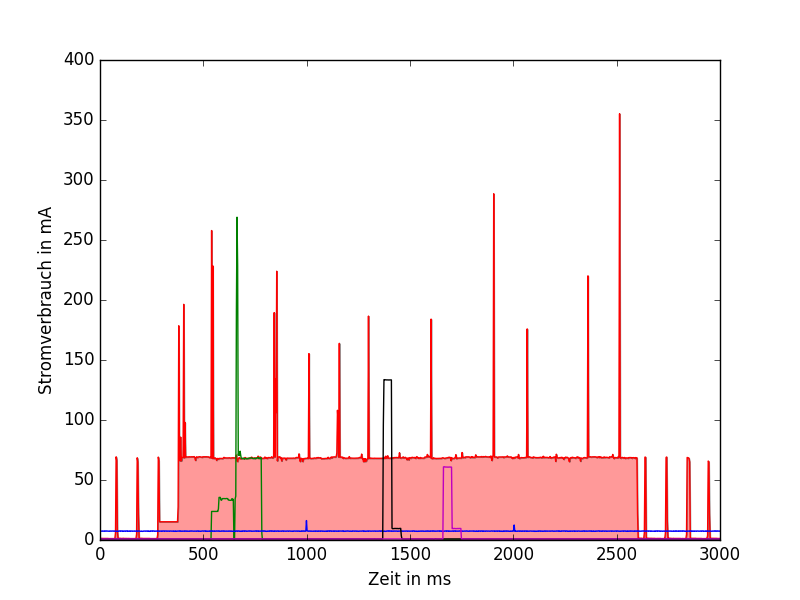
\includegraphics[width=\textwidth]{plots/alle.png}
  \caption{Stromverbrauchskurven für den Ortungsvorgang im Vergleich. Rot: \emph{WiFi-LLS}; Grün: \emph{Probe-Request-Lokalisierung}; Blau: \emph{BLE-Advertising}; Schwarz: LoRa 23 dBm; Lila: LoRa 5 dBm.}
  \label{fig:alle}
\end{figure}


\section{Auswertung}
Es wurden mobile Einheiten mit IEEE 802.11, Bluetooth Low Energy (BLE) und Long Range (LoRa) implementiert und bezüglich ihrer Reichweite und ihres Energieverbrauchs untersucht.

IEEE 802.11 ist den anderen Protokollen weder bei der Reichweite, noch beim Energieverbrauch überlegen. 
Sein Vorteil liegt in der Verfügbarkeit von WLAN \emph{Access Points} (APs), welche als Basisstationen verwendet werden können.
IEEE 802.11 hat jedoch im gegebenen Szenario für den Tunnelbau Probleme mit Bereichen, die durch das WLAN-Netzwerk nicht abgedeckt sind. 
Diese können vermieden werden, wenn spezielle Funktionen beim AP vorausgesetzt werden können.

BLE zeichnet sich durch einen niedrigen Energieverbrauch pro Sendevorgang aus, allerdings zeigte sich bei der Prüfung der Reichweite von BLE auch, dass diese mit 14 bis 32 m nicht sehr groß ist.
Dies wirkt sich negativ auf die Erkennungszuverlässigkeit bei Bereichswechseln aus, außerdem gibt es dadurch große Bereiche, in denen die mobilen Einheiten nicht geortet werden können.

Dieses Problem hat LoRa nicht. 
Seine enorme Reichweite von bis zu 1250 m erlaubt es, dass eine mobile Einheit an jedem Punkt im Tunnel von mehreren Basisstationen geortet werden kann.
Diese Eigenschaft macht die mobile Einheit mit LoRa zu einer sehr zuverlässigen Einheit für die Ortung.
Beachtet werden muss jedoch, dass LoRa Kollisionen nur durch die zufällige Wahl des Kanals zu verhindern versucht.
Es muss daher mit gelegentlichen Kollisionen gerechnet werden.
Daher sollte das Sendeintervall auf die Hälfte des gewünschten Ortungsintervalls gesetzt werden, um eine zuverlässige Ortung im Ortungsintervall zu erreichen.

Aufgrund seiner hohen Reichweite und daraus resultierenden lückenlosen Ortung der mobilen Einheiten, schlägt diese Arbeit LoRa für \emph{zuverlässige funkbasierte Bereichsortung im Tunnelbau} vor.






\chapter{Beschleunigungssensor}
\label{ch:Beschleunigungssensor}
Um den Energieverbrauch der WLAN-basierten Lösungen zu senken wird in diesem Kapitel die Einbindung eines Beschleunigungssensors diskutiert. \\
Im Tunnel Rastatt, in dem auch die Versuche stattfanden, arbeiten die Bauarbeiter in zwei Schichten zu je zwölf Stunden. 
Nach zehn Tagen Schicht hat ein Arbeiter fünf Tage frei, jeder Arbeiter arbeitet also genau ein Drittel der Gesamtzeit. \\
Die mobile Einheit behält jedoch derzeit seinen Senderythmus bei, angesichts des hohen Stromverbrauchs beim Senden ist dies ineffizient.
Ein Beschleunigungssensor soll bestimmen, wann die mobile Einheit in Bewegung ist. 
Dadurch wird sie nicht mehr senden, wenn sie nicht getragen wird.

\section{LIS3DH}
Der LIS3DH ist ein drei Achsen Beschleunigungssensor von ST Microelectronics \cite{st2015lis}.
Er zeichnet sich durch einen ultra-low-power Modus und einen Pin für externe Unterbrechung (interrupt) aus.
Der Beschleunigungssensor bietet ein $I^2C$ und ein SPI Interface um ihn zu konfigurieren.
Der LIS3DH benötigt bei einer Frequenz von einem Herz nur 2 Mikroamper (0,002 mA).\\
Leider konnte bei Laufbewegungen bei einem Herz nicht sicher der interrupt ausgelöst werden, die Frequenz wurde deshalb auf zehn Herz erhöht.
Für eine Frequenz von zehn Herz im ultra-low-power Modus listet das Datenblatt einen Verbrauch von 3 Mikroamper.

\section{Abschaltautomatik}
\label{ch:Beschleunigungssensor:sec:Abschaltautomatik}
Der ESP8266 besitzt einen Enable Pin, ist dieser mit der Versorungsspannung verbunden werden die internen Spannungregler aktiviert und der ESP8266 mit Strom versorgt.
Die eigentliche Stromversorgung bezieht er dabei jedoch aus dem Vcc Pin.
Der ESP8266 soll durch den LIS3DH angeschaltet werden, dieser darf die Stromversorgung bei Bedarf trennen, sie kann danach wieder vom LIS3DH wieder aktiviert werden. \\
Um dieses Verhalten zu erreichen wird ein Latch eingesetzt \cite{texas2003latch}.
Es handelt sich dabei um einen digitalen Schalter mit einem SET Eingang (An), einem RESET Eingang (Aus) und einem Ausgang.
Der Ausgang wird mit dem Enable Pin verbunden, ist er aktiv, wird der ESP8266 aktiv.
Der SET Eingang wird mit dem interrupt Pin des LIS3DH verbunden, er kann damit den den Ausgang aktivieren.
Der RESET Eingang wird mit dem ESP8266 verbunden. 
Es wurde Pin 16 ausgewählt, da dieser für das Aufwecken aus dem Tiefschlaf zuständig ist. 
Stattdessen soll er nun die Stromversorgung abschalten und durch die zuvor im \texttt{deep\_sleep} verbrachte Zeit das Sendeintervall abwarten.\\
Da das Aufwecken mit Pin 16 durch das Verbinden des Pins mit der Masse funktioniert, kann damit nicht direkt der RESET Eingang des Latches betrieben werden.
Stattdessen wird das Ergebnis von Pin 16 mit der Versorgungsspannung über ein XOR Gatter verschaltet und mit dem RESET Eingang verbunden \cite{texas2014xor}.

\section{Bewertung}
Der Verbrauch des Beschleunigungssensors ersetzt lediglich den Verbrauch des Mikrocontrollers, die anderen Komponenten bleiben davon unberührt.
Zu den 3 Mikroamper Verbrauch addiert sich deshalb der Verbrauch des Spannungswandlers (55 Mikroamper) und des Lithium-Polymer-Ladeschaltkreises (bis zu 100 Mirkoamper).
Hinzu kommen bis zu 1 Mikroamper für das Latch und 10 Mikroamper für das XOR Gatter.\\
Die Integration des Beschleunigungssensor kann also den Verbrauch des ESP8266 außerhalb der Arbeitszeiten durch einen Verbrauch von 14 Mikroamper ersetzen, die bis zu 155 Mikroamper Verbrauch der umliegenden Komponenten bleibt jedoch vorhanden.
Die Laufzeit für eine nicht bewegte mobilen Einheit mit ESP8266 beträgt dann mindestens $1400mAh / 0,169mA = 8284h$, dies entspricht ca. 345 Tagen.\\
Für die mobile Einheit mit nRF52 macht die Integration des Beschleunigungssensors keinen Sinn, da der mittlere Verbrauch dieses Mikrocontrollers nur ca. 2 Mikroamper über dem des Beschleunigungssensors liegt.


\chapter{Fazit}
\label{ch:Fazit}
In dieser Arbeit wurden nach der Einleitung zunächst die Grundlagen funkbasierter Ortung und ausgewählter Funkprotokolle erörtert.
Diese waren IEEE 802.11, Bluetooth Low Energy (BLE) und Long Range (LoRa).
Anschließend wurden verwandte Arbeiten analysiert und eine Auswahl an Verfahren für die nachfolgenden Implementierungen gewählt.
Jedes der ausgewählten Protokollen wurde auf seine Reichweite im Tunnel hin untersucht.
Zusätzlich wurde für jede Implementierung der Stromverbrauch untersucht.

In dieser Arbeit hatte LoRa die höchste Reichweite im Tunnel, BLE hatte die geringste Reichweite.
Im Gegenzug hatte BLE aber den niedrigsten Stromverbrauch, IEEE 802.11 hatte bei geringerer Reichweite einen höheren Stromvebrauch als LoRa.

Diese Arbeit schlägt LoRa für \emph{zuverlässige funkbasierte Bereichsortung im Tunnelbau} vor, da die Reichweite bei hohen Sendeleistungen ausreicht mehrere Basisstationen zu erreichen. 
Dies erlaubt eine Zuverlässigkeit bei der Ortung, die die lückenhafte Ortung mit IEEE 802.11 und BLE nicht erreichen können.

\section{Ausblick}
Neben den drei Protokollen, die in dieser Arbeit untersucht wurden, eignen sich viele weitere grundsätzlich für die Bereichsortung.
Für zukünftige Arbeiten könnten daher noch viele weitere Protokolle untersucht werden. 

Außerdem kann, gegeben der hohen Reichweiten von LoRa, der Umstieg von Bereichsortung auf geometrische Ortung für den Tunnelbau diskutiert werden. 
Das Erreichen mehrerer Basisstationen erlaubt nun eine Triangulation der Position der mobilen Einheit.
Dazu müssten die Messgrößen von LoRa (oder einem anderen Protokoll mit sehr hoher Reichweite) auf ihre Eignung für die Lokalisierung geprüft werden und geeignete Modelle für die Signalausbreitung im Tunnel sowie der Einfluss von dynamischen Hindernissen erstellt werden.



%% ++++++++++++++++++++++++++++++++++++++++++
%% Anhang
%% ++++++++++++++++++++++++++++++++++++++++++

\appendix
%\include{anhang_a}
%\include{anhang_b}

%% ++++++++++++++++++++++++++++++++++++++++++
%% Literatur
%% ++++++++++++++++++++++++++++++++++++++++++
%  mit dem Befehl \nocite werden auch nicht 
%  zitierte Referenzen abgedruckt
\cleardoublepage
\phantomsection
\addcontentsline{toc}{chapter}{\bibname}
%%
%\nocite{*} % nur angeben, wenn auch nicht im Text zitierte Quellen 
           % erscheinen sollen
\bibliographystyle{itmabbrv} % mit abgekürzten Vornamen der Autoren
%\bibliographystyle{gerplain} % abbrvnat unsrtnat
% spezielle Zitierstile: Labels mit vier Buchstaben und Jahreszahl
%\bibliographystyle{itmalpha}  % ausgeschriebene Vornamen der Autoren
\bibliography{thesis}
%% ++++++++++++++++++++++++++++++++++++++++++
%% Index
%% ++++++++++++++++++++++++++++++++++++++++++
\ifnotdraft{
\cleardoublepage
\phantomsection
\printindex            % Index, Stichwortverzeichnis
}
\end{document}
%% end of file
